\documentclass{whiteboard}
\begin{document}
\begin{frame}[plain,t]
\bbcover{Grafos}{Programação Dinâmica em DAGs}{Prof. Edson Alves}{Faculdade UnB Gama}

\end{frame}
\begin{frame}[plain,t]
\begin{tikzpicture}
\node[draw,opacity=0] at (0, 0) {x};
\node[draw,opacity=0] at (14, 8) {x};

	\node[anchor=west] (title) at (0.0, 6.0) { \Large \bbbold{Relação entre DAGs e programação dinâmica} };
\end{tikzpicture}
\end{frame}
\begin{frame}[plain,t]
\begin{tikzpicture}
\node[draw,opacity=0] at (0, 0) {x};
\node[draw,opacity=0] at (14, 8) {x};

	\node[anchor=west] (title) at (0.0, 6.0) { \Large \bbbold{Relação entre DAGs e programação dinâmica} };

	\node[anchor=west] (a) at (1.0, 5.0) { $\star$ \bbtext{É possível utilizar algoritmos de programação (DP) dinâmica em um grafo } };

	\node[anchor=west] (a1) at (0.5, 4.5) { \bbtext{$G$, se $G$ é direcionado e acíclico (DAG -- \bbenglish{directed acyclic graph})} };

\end{tikzpicture}
\end{frame}
\begin{frame}[plain,t]
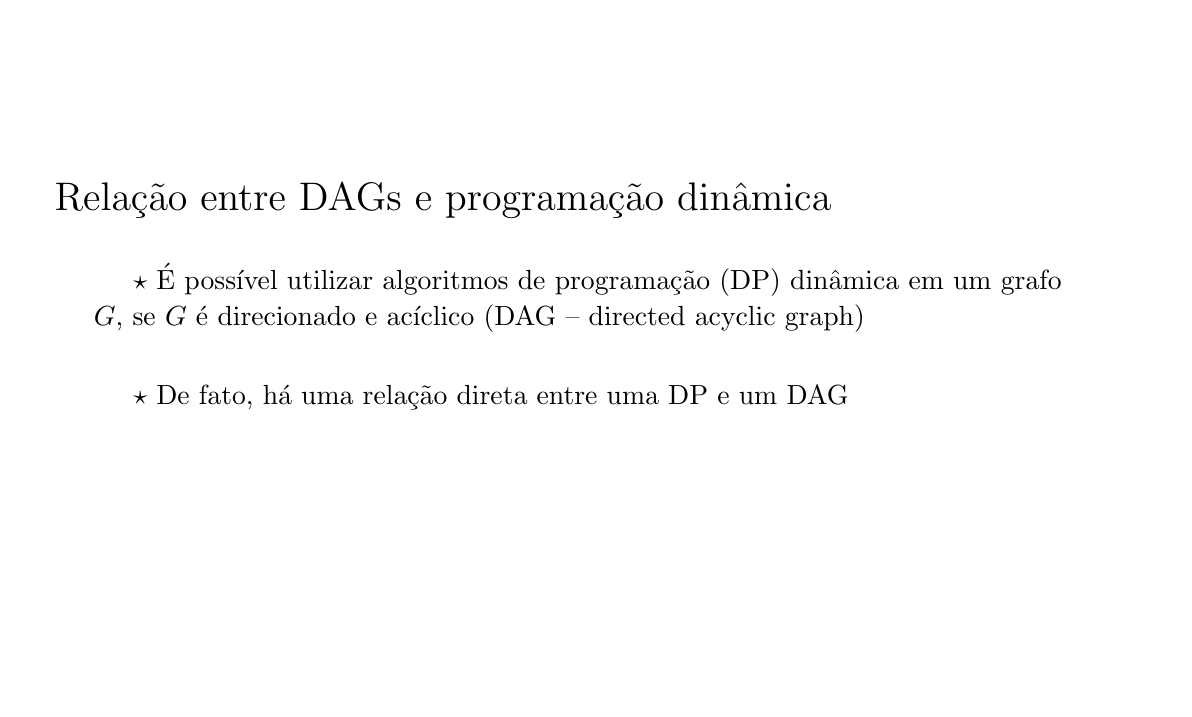
\begin{tikzpicture}
\node[draw,opacity=0] at (0, 0) {x};
\node[draw,opacity=0] at (14, 8) {x};

	\node[anchor=west] (title) at (0.0, 6.0) { \Large \bbbold{Relação entre DAGs e programação dinâmica} };

	\node[anchor=west] (a) at (1.0, 5.0) { $\star$ \bbtext{É possível utilizar algoritmos de programação (DP) dinâmica em um grafo } };

	\node[anchor=west] (a1) at (0.5, 4.5) { \bbtext{$G$, se $G$ é direcionado e acíclico (DAG -- \bbenglish{directed acyclic graph})} };


	\node[anchor=west] (b) at (1.0, 3.5) { $\star$ \bbtext{De fato, há uma relação direta entre uma DP e um DAG} };

\end{tikzpicture}
\end{frame}
\begin{frame}[plain,t]
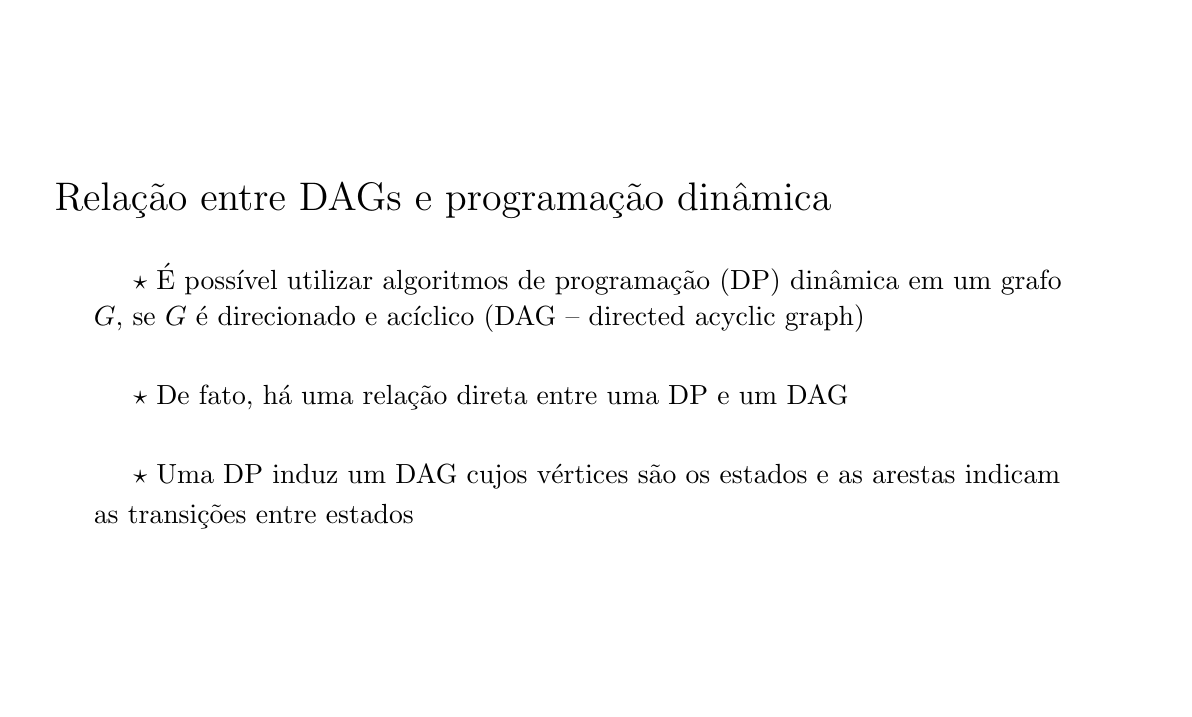
\begin{tikzpicture}
\node[draw,opacity=0] at (0, 0) {x};
\node[draw,opacity=0] at (14, 8) {x};

	\node[anchor=west] (title) at (0.0, 6.0) { \Large \bbbold{Relação entre DAGs e programação dinâmica} };

	\node[anchor=west] (a) at (1.0, 5.0) { $\star$ \bbtext{É possível utilizar algoritmos de programação (DP) dinâmica em um grafo } };

	\node[anchor=west] (a1) at (0.5, 4.5) { \bbtext{$G$, se $G$ é direcionado e acíclico (DAG -- \bbenglish{directed acyclic graph})} };


	\node[anchor=west] (b) at (1.0, 3.5) { $\star$ \bbtext{De fato, há uma relação direta entre uma DP e um DAG} };


	\node[anchor=west] (c) at (1.0, 2.5) { $\star$ \bbtext{Uma DP induz um DAG cujos vértices são os estados e as arestas indicam} };

	\node[anchor=west] (c1) at (0.5, 2.0) { \bbtext{as transições entre estados} };

\end{tikzpicture}
\end{frame}
\begin{frame}[plain,t]
\begin{tikzpicture}
\node[draw,opacity=0] at (0, 0) {x};
\node[draw,opacity=0] at (14, 8) {x};

	\node[anchor=west] (title) at (0.0, 6.0) { \Large \bbbold{Aplicação: número de caminhos de $u$ a $v$} };
\end{tikzpicture}
\end{frame}
\begin{frame}[plain,t]
\begin{tikzpicture}
\node[draw,opacity=0] at (0, 0) {x};
\node[draw,opacity=0] at (14, 8) {x};

	\node[anchor=west] (title) at (0.0, 6.0) { \Large \bbbold{Aplicação: número de caminhos de $u$ a $v$} };

	\node[anchor=west] (a) at (1.0, 5.0) { $\star$ \bbtext{É possível computar o número de caminhos distintos entre os vértices} };

	\node[anchor=west] (a1) at (0.5, 4.5) { \bbtext{$u, v\in V$ de um DAG $G(V, E)$} };

\end{tikzpicture}
\end{frame}
\begin{frame}[plain,t]
\begin{tikzpicture}
\node[draw,opacity=0] at (0, 0) {x};
\node[draw,opacity=0] at (14, 8) {x};

	\node[anchor=west] (title) at (0.0, 6.0) { \Large \bbbold{Aplicação: número de caminhos de $u$ a $v$} };

	\node[anchor=west] (a) at (1.0, 5.0) { $\star$ \bbtext{É possível computar o número de caminhos distintos entre os vértices} };

	\node[anchor=west] (a1) at (0.5, 4.5) { \bbtext{$u, v\in V$ de um DAG $G(V, E)$} };


	\node[anchor=west] (b) at (1.0, 3.5) { $\star$ \bbtext{Seja $p_u(x)$ o número de caminhos de $u$ a $x$} };

\end{tikzpicture}
\end{frame}
\begin{frame}[plain,t]
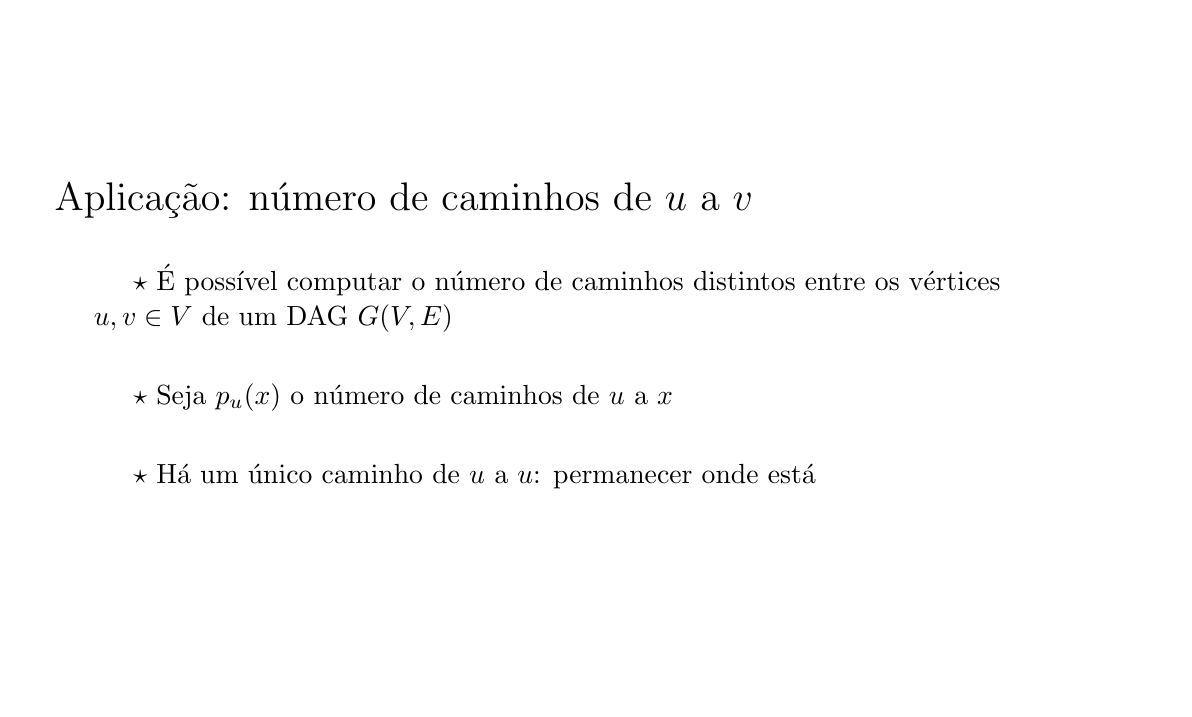
\begin{tikzpicture}
\node[draw,opacity=0] at (0, 0) {x};
\node[draw,opacity=0] at (14, 8) {x};

	\node[anchor=west] (title) at (0.0, 6.0) { \Large \bbbold{Aplicação: número de caminhos de $u$ a $v$} };

	\node[anchor=west] (a) at (1.0, 5.0) { $\star$ \bbtext{É possível computar o número de caminhos distintos entre os vértices} };

	\node[anchor=west] (a1) at (0.5, 4.5) { \bbtext{$u, v\in V$ de um DAG $G(V, E)$} };


	\node[anchor=west] (b) at (1.0, 3.5) { $\star$ \bbtext{Seja $p_u(x)$ o número de caminhos de $u$ a $x$} };


	\node[anchor=west] (c) at (1.0, 2.5) { $\star$ \bbtext{Há um único caminho de $u$ a $u$:  permanecer onde está} };

\end{tikzpicture}
\end{frame}
\begin{frame}[plain,t]
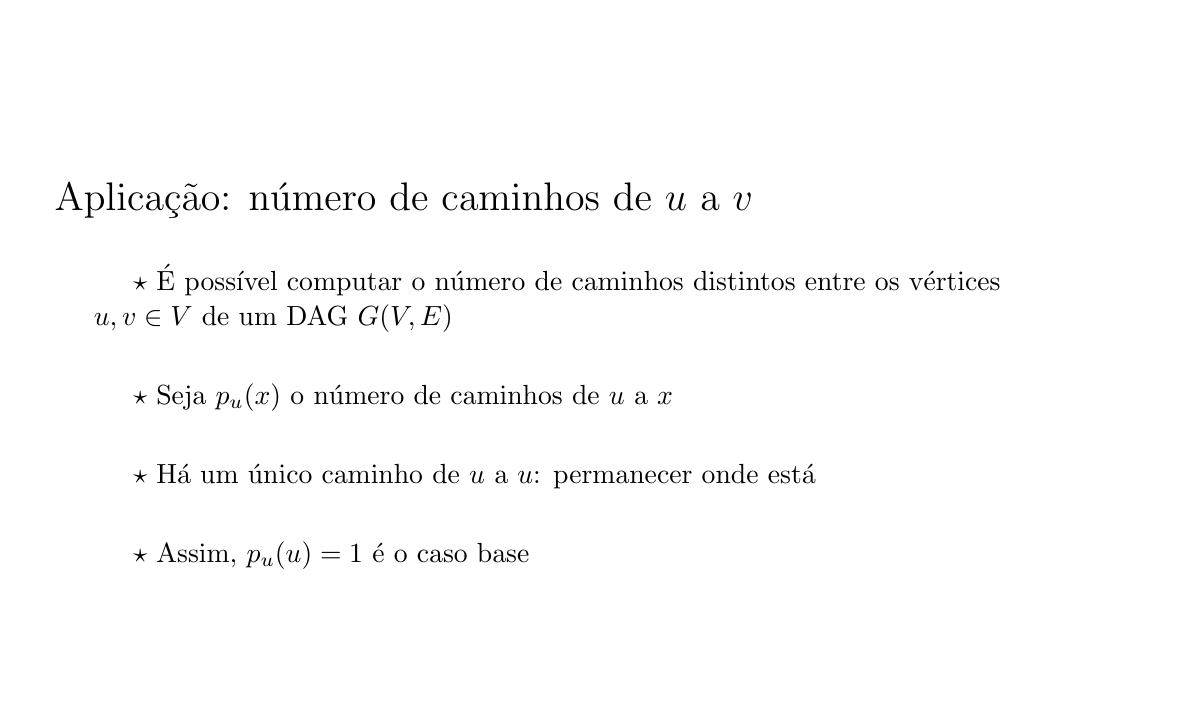
\begin{tikzpicture}
\node[draw,opacity=0] at (0, 0) {x};
\node[draw,opacity=0] at (14, 8) {x};

	\node[anchor=west] (title) at (0.0, 6.0) { \Large \bbbold{Aplicação: número de caminhos de $u$ a $v$} };

	\node[anchor=west] (a) at (1.0, 5.0) { $\star$ \bbtext{É possível computar o número de caminhos distintos entre os vértices} };

	\node[anchor=west] (a1) at (0.5, 4.5) { \bbtext{$u, v\in V$ de um DAG $G(V, E)$} };


	\node[anchor=west] (b) at (1.0, 3.5) { $\star$ \bbtext{Seja $p_u(x)$ o número de caminhos de $u$ a $x$} };


	\node[anchor=west] (c) at (1.0, 2.5) { $\star$ \bbtext{Há um único caminho de $u$ a $u$:  permanecer onde está} };


	\node[anchor=west] (d) at (1.0, 1.5) { $\star$ \bbtext{Assim, $p_u(u) = 1$ é o caso base} };

\end{tikzpicture}
\end{frame}
\begin{frame}[plain,t]
\begin{tikzpicture}
\node[draw,opacity=0] at (0, 0) {x};
\node[draw,opacity=0] at (14, 8) {x};

	\node[anchor=west] (title) at (0.0, 6.0) { \Large \bbbold{Aplicação: número de caminhos de $u$ a $v$} };

	\node[anchor=west] (a) at (1.0, 5.0) { $\star$ \bbtext{Para os demais vértices $x\in V$, vale que} };

	\node[] (a1) at (7.0, 4.0) { $\displaystyle p_u(x) = \sum_{(v_i, x)\in E} p_u(v_i)$ };

\end{tikzpicture}
\end{frame}
\begin{frame}[plain,t]
\begin{tikzpicture}
\node[draw,opacity=0] at (0, 0) {x};
\node[draw,opacity=0] at (14, 8) {x};

	\node[anchor=west] (title) at (0.0, 6.0) { \Large \bbbold{Aplicação: número de caminhos de $u$ a $v$} };

	\node[anchor=west] (a) at (1.0, 5.0) { $\star$ \bbtext{Para os demais vértices $x\in V$, vale que} };

	\node[] (a1) at (7.0, 4.0) { $\displaystyle p_u(x) = \sum_{(v_i, x)\in E} p_u(v_i)$ };


	\node[anchor=west] (b) at (1.0, 3.0) { $\star$ \bbtext{O cálculo de $p_u(x)$ depende da ordem de processamento dos vértices} };

\end{tikzpicture}
\end{frame}
\begin{frame}[plain,t]
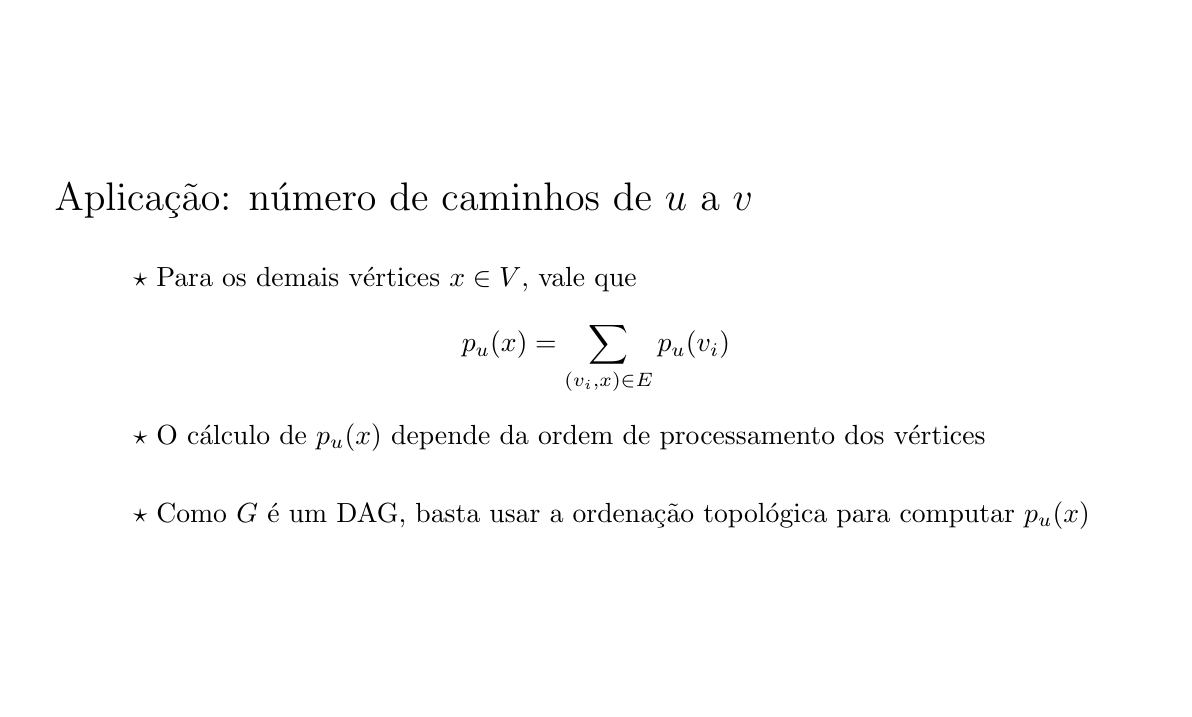
\begin{tikzpicture}
\node[draw,opacity=0] at (0, 0) {x};
\node[draw,opacity=0] at (14, 8) {x};

	\node[anchor=west] (title) at (0.0, 6.0) { \Large \bbbold{Aplicação: número de caminhos de $u$ a $v$} };

	\node[anchor=west] (a) at (1.0, 5.0) { $\star$ \bbtext{Para os demais vértices $x\in V$, vale que} };

	\node[] (a1) at (7.0, 4.0) { $\displaystyle p_u(x) = \sum_{(v_i, x)\in E} p_u(v_i)$ };


	\node[anchor=west] (b) at (1.0, 3.0) { $\star$ \bbtext{O cálculo de $p_u(x)$ depende da ordem de processamento dos vértices} };


	\node[anchor=west] (c) at (1.0, 2.0) { $\star$ \bbtext{Como $G$ é um DAG, basta usar a ordenação topológica para computar $p_u(x)$} };

\end{tikzpicture}
\end{frame}
\begin{frame}[plain,t]
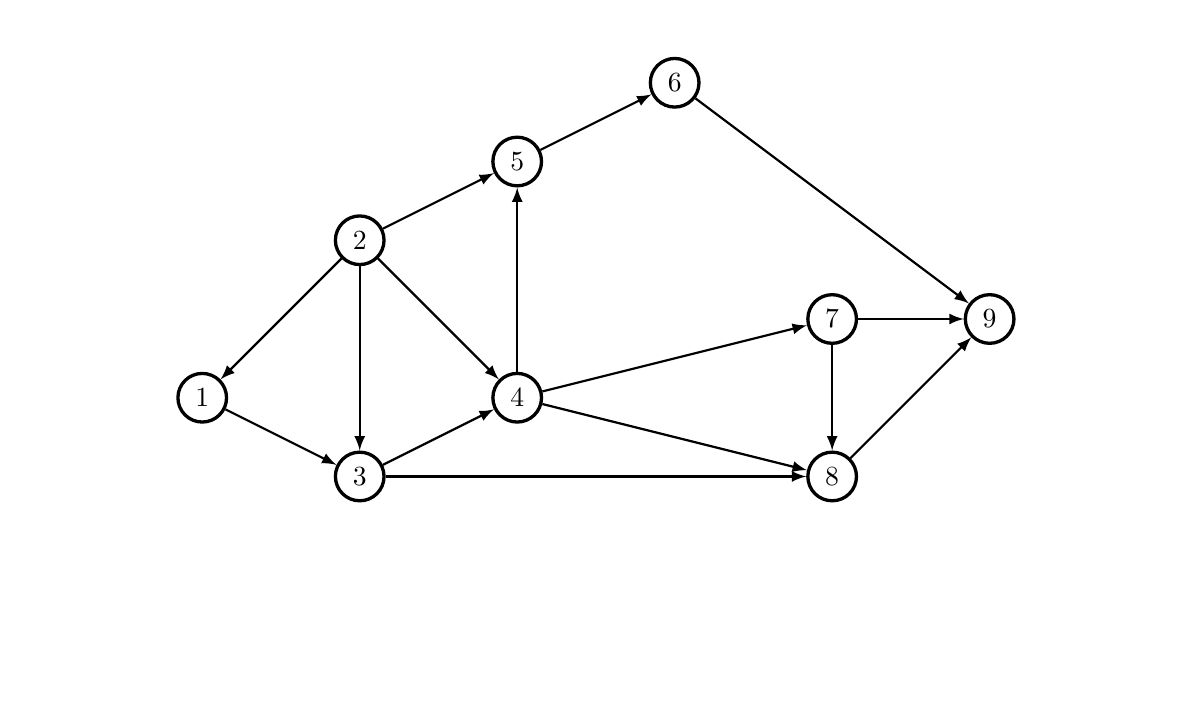
\begin{tikzpicture}
\node[draw,opacity=0] at (0, 0) {x};
\node[draw,opacity=0] at (14, 8) {x};

	\node[very thick,draw,circle] (node1) at (2.0, 3.5) { \bbtext{1} };

	\node[very thick,draw,circle] (node2) at (4.0, 5.5) { \bbtext{2} };

	\node[very thick,draw,circle] (node3) at (4.0, 2.5) { \bbtext{3} };

	\node[very thick,draw,circle] (node4) at (6.0, 3.5) { \bbtext{4} };

	\node[very thick,draw,circle] (node5) at (6.0, 6.5) { \bbtext{5} };

	\node[very thick,draw,circle] (node6) at (8.0, 7.5) { \bbtext{6} };

	\node[very thick,draw,circle] (node7) at (10.0, 4.5) { \bbtext{7} };

	\node[very thick,draw,circle] (node8) at (10.0, 2.5) { \bbtext{8} };

	\node[very thick,draw,circle] (node9) at (12.0, 4.5) { \bbtext{9} };


	\draw[thick,-latex](node2) to (node1);

	\draw[thick,-latex](node2) to (node3);

	\draw[thick,-latex](node2) to (node4);

	\draw[thick,-latex](node2) to (node5);

	\draw[thick,-latex](node1) to (node3);

	\draw[thick,-latex](node3) to (node4);

	\draw[thick,-latex](node3) to (node8);

	\draw[thick,-latex](node4) to (node5);

	\draw[thick,-latex](node4) to (node7);

	\draw[thick,-latex](node4) to (node8);

	\draw[thick,-latex](node5) to (node6);

	\draw[thick,-latex](node6) to (node9);

	\draw[thick,-latex](node7) to (node8);

	\draw[thick,-latex](node7) to (node9);

	\draw[thick,-latex](node8) to (node9);


\end{tikzpicture}
\end{frame}
\begin{frame}[plain,t]
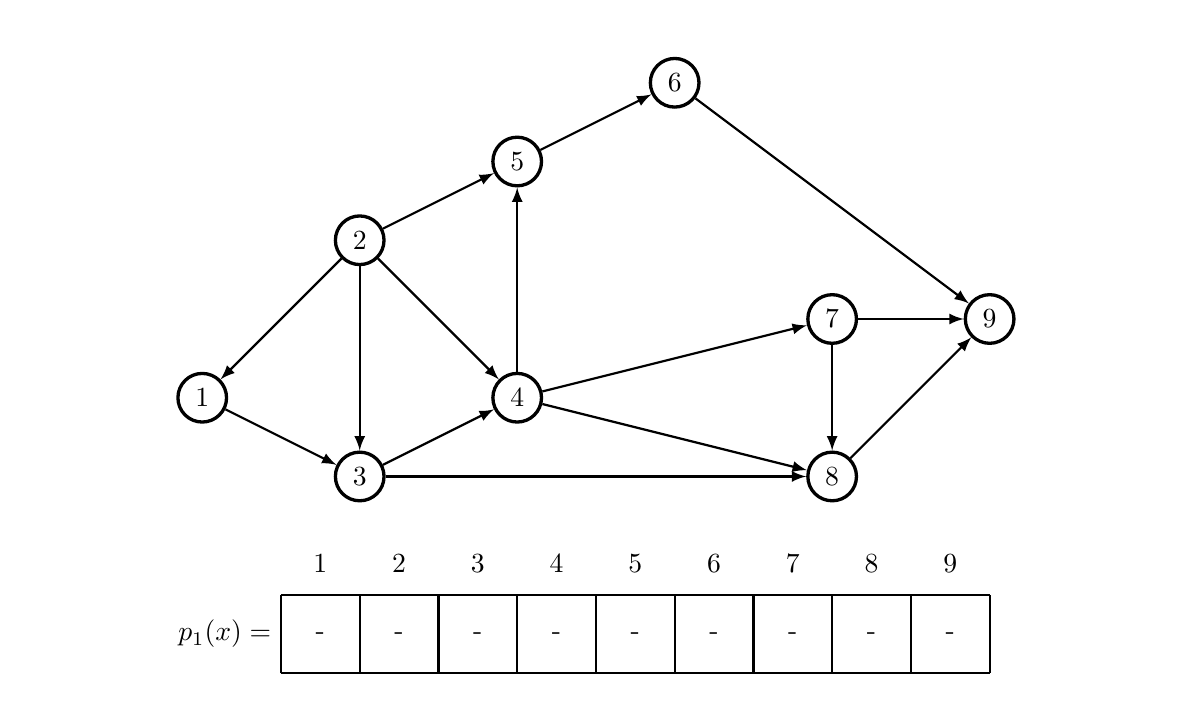
\begin{tikzpicture}
\node[draw,opacity=0] at (0, 0) {x};
\node[draw,opacity=0] at (14, 8) {x};

	\node[very thick,draw,circle] (node1) at (2.0, 3.5) { \bbtext{1} };

	\node[very thick,draw,circle] (node2) at (4.0, 5.5) { \bbtext{2} };

	\node[very thick,draw,circle] (node3) at (4.0, 2.5) { \bbtext{3} };

	\node[very thick,draw,circle] (node4) at (6.0, 3.5) { \bbtext{4} };

	\node[very thick,draw,circle] (node5) at (6.0, 6.5) { \bbtext{5} };

	\node[very thick,draw,circle] (node6) at (8.0, 7.5) { \bbtext{6} };

	\node[very thick,draw,circle] (node7) at (10.0, 4.5) { \bbtext{7} };

	\node[very thick,draw,circle] (node8) at (10.0, 2.5) { \bbtext{8} };

	\node[very thick,draw,circle] (node9) at (12.0, 4.5) { \bbtext{9} };


	\draw[thick,-latex](node2) to (node1);

	\draw[thick,-latex](node2) to (node3);

	\draw[thick,-latex](node2) to (node4);

	\draw[thick,-latex](node2) to (node5);

	\draw[thick,-latex](node1) to (node3);

	\draw[thick,-latex](node3) to (node4);

	\draw[thick,-latex](node3) to (node8);

	\draw[thick,-latex](node4) to (node5);

	\draw[thick,-latex](node4) to (node7);

	\draw[thick,-latex](node4) to (node8);

	\draw[thick,-latex](node5) to (node6);

	\draw[thick,-latex](node6) to (node9);

	\draw[thick,-latex](node7) to (node8);

	\draw[thick,-latex](node7) to (node9);

	\draw[thick,-latex](node8) to (node9);



	\draw[thick] (3.0, 0.0) grid  (12.0, 1.0);

	\node[anchor=east] (p) at (3.0, 0.5) { $p_1(x) = $ };

	\node[] (x1) at (3.5, 1.4) { \bbtext{1} };

	\node[] (x2) at (4.5, 1.4) { \bbtext{2} };

	\node[] (x3) at (5.5, 1.4) { \bbtext{3} };

	\node[] (x4) at (6.5, 1.4) { \bbtext{4} };

	\node[] (x5) at (7.5, 1.4) { \bbtext{5} };

	\node[] (x6) at (8.5, 1.4) { \bbtext{6} };

	\node[] (x7) at (9.5, 1.4) { \bbtext{7} };

	\node[] (x8) at (10.5, 1.4) { \bbtext{8} };

	\node[] (x9) at (11.5, 1.4) { \bbtext{9} };

	\node[] (d1) at (3.5, 0.5) { \bbtext{-} };

	\node[] (d2) at (4.5, 0.5) { \bbtext{-} };

	\node[] (d3) at (5.5, 0.5) { \bbtext{-} };

	\node[] (d4) at (6.5, 0.5) { \bbtext{-} };

	\node[] (d5) at (7.5, 0.5) { \bbtext{-} };

	\node[] (d6) at (8.5, 0.5) { \bbtext{-} };

	\node[] (d7) at (9.5, 0.5) { \bbtext{-} };

	\node[] (d8) at (10.5, 0.5) { \bbtext{-} };

	\node[] (d9) at (11.5, 0.5) { \bbtext{-} };

\end{tikzpicture}
\end{frame}
\begin{frame}[plain,t]
\begin{tikzpicture}
\node[draw,opacity=0] at (0, 0) {x};
\node[draw,opacity=0] at (14, 8) {x};

	\node[very thick,draw,circle,fill=BBCyan] (node1) at (2.0, 3.5) { \bbtext{1} };

	\node[very thick,draw,circle] (node2) at (4.0, 5.5) { \bbtext{2} };

	\node[very thick,draw,circle] (node3) at (4.0, 2.5) { \bbtext{3} };

	\node[very thick,draw,circle] (node4) at (6.0, 3.5) { \bbtext{4} };

	\node[very thick,draw,circle] (node5) at (6.0, 6.5) { \bbtext{5} };

	\node[very thick,draw,circle] (node6) at (8.0, 7.5) { \bbtext{6} };

	\node[very thick,draw,circle] (node7) at (10.0, 4.5) { \bbtext{7} };

	\node[very thick,draw,circle] (node8) at (10.0, 2.5) { \bbtext{8} };

	\node[very thick,draw,circle] (node9) at (12.0, 4.5) { \bbtext{9} };


	\draw[thick,-latex](node2) to (node1);

	\draw[thick,-latex](node2) to (node3);

	\draw[thick,-latex](node2) to (node4);

	\draw[thick,-latex](node2) to (node5);

	\draw[thick,-latex](node1) to (node3);

	\draw[thick,-latex](node3) to (node4);

	\draw[thick,-latex](node3) to (node8);

	\draw[thick,-latex](node4) to (node5);

	\draw[thick,-latex](node4) to (node7);

	\draw[thick,-latex](node4) to (node8);

	\draw[thick,-latex](node5) to (node6);

	\draw[thick,-latex](node6) to (node9);

	\draw[thick,-latex](node7) to (node8);

	\draw[thick,-latex](node7) to (node9);

	\draw[thick,-latex](node8) to (node9);



	\draw[thick] (3.0, 0.0) grid  (12.0, 1.0);

	\node[anchor=east] (p) at (3.0, 0.5) { $p_1(x) = $ };

	\node[] (x1) at (3.5, 1.4) { \bbtext{1} };

	\node[] (x2) at (4.5, 1.4) { \bbtext{2} };

	\node[] (x3) at (5.5, 1.4) { \bbtext{3} };

	\node[] (x4) at (6.5, 1.4) { \bbtext{4} };

	\node[] (x5) at (7.5, 1.4) { \bbtext{5} };

	\node[] (x6) at (8.5, 1.4) { \bbtext{6} };

	\node[] (x7) at (9.5, 1.4) { \bbtext{7} };

	\node[] (x8) at (10.5, 1.4) { \bbtext{8} };

	\node[] (x9) at (11.5, 1.4) { \bbtext{9} };

	\node[] (d1) at (3.5, 0.5) { $\mathbf{1}$ };

	\node[] (d2) at (4.5, 0.5) { \bbtext{-} };

	\node[] (d3) at (5.5, 0.5) { \bbtext{-} };

	\node[] (d4) at (6.5, 0.5) { \bbtext{-} };

	\node[] (d5) at (7.5, 0.5) { \bbtext{-} };

	\node[] (d6) at (8.5, 0.5) { \bbtext{-} };

	\node[] (d7) at (9.5, 0.5) { \bbtext{-} };

	\node[] (d8) at (10.5, 0.5) { \bbtext{-} };

	\node[] (d9) at (11.5, 0.5) { \bbtext{-} };



\end{tikzpicture}
\end{frame}
\begin{frame}[plain,t]
\begin{tikzpicture}
\node[draw,opacity=0] at (0, 0) {x};
\node[draw,opacity=0] at (14, 8) {x};

	\node[very thick,draw,circle,fill=BBCyan] (node1) at (2.0, 3.5) { \bbtext{1} };

	\node[very thick,draw,circle] (node2) at (4.0, 5.5) { \bbtext{2} };

	\node[very thick,draw,circle] (node3) at (4.0, 2.5) { \bbtext{3} };

	\node[very thick,draw,circle] (node4) at (6.0, 3.5) { \bbtext{4} };

	\node[very thick,draw,circle] (node5) at (6.0, 6.5) { \bbtext{5} };

	\node[very thick,draw,circle] (node6) at (8.0, 7.5) { \bbtext{6} };

	\node[very thick,draw,circle] (node7) at (10.0, 4.5) { \bbtext{7} };

	\node[very thick,draw,circle] (node8) at (10.0, 2.5) { \bbtext{8} };

	\node[very thick,draw,circle] (node9) at (12.0, 4.5) { \bbtext{9} };

	\node[anchor=west] (O) at (0.0, 7.5) { \bbtext{$O = \{$ 2, 1, 3, 4, 7, 8, 5, 6, 9 $\}$} };

	\draw[thick,-latex](node2) to (node1);

	\draw[thick,-latex](node2) to (node3);

	\draw[thick,-latex](node2) to (node4);

	\draw[thick,-latex](node2) to (node5);

	\draw[thick,-latex](node1) to (node3);

	\draw[thick,-latex](node3) to (node4);

	\draw[thick,-latex](node3) to (node8);

	\draw[thick,-latex](node4) to (node5);

	\draw[thick,-latex](node4) to (node7);

	\draw[thick,-latex](node4) to (node8);

	\draw[thick,-latex](node5) to (node6);

	\draw[thick,-latex](node6) to (node9);

	\draw[thick,-latex](node7) to (node8);

	\draw[thick,-latex](node7) to (node9);

	\draw[thick,-latex](node8) to (node9);



	\draw[thick] (3.0, 0.0) grid  (12.0, 1.0);

	\node[anchor=east] (p) at (3.0, 0.5) { $p_1(x) = $ };

	\node[] (x1) at (3.5, 1.4) { \bbtext{1} };

	\node[] (x2) at (4.5, 1.4) { \bbtext{2} };

	\node[] (x3) at (5.5, 1.4) { \bbtext{3} };

	\node[] (x4) at (6.5, 1.4) { \bbtext{4} };

	\node[] (x5) at (7.5, 1.4) { \bbtext{5} };

	\node[] (x6) at (8.5, 1.4) { \bbtext{6} };

	\node[] (x7) at (9.5, 1.4) { \bbtext{7} };

	\node[] (x8) at (10.5, 1.4) { \bbtext{8} };

	\node[] (x9) at (11.5, 1.4) { \bbtext{9} };

	\node[] (d1) at (3.5, 0.5) { $\mathbf{1}$ };

	\node[] (d2) at (4.5, 0.5) { \bbtext{-} };

	\node[] (d3) at (5.5, 0.5) { \bbtext{-} };

	\node[] (d4) at (6.5, 0.5) { \bbtext{-} };

	\node[] (d5) at (7.5, 0.5) { \bbtext{-} };

	\node[] (d6) at (8.5, 0.5) { \bbtext{-} };

	\node[] (d7) at (9.5, 0.5) { \bbtext{-} };

	\node[] (d8) at (10.5, 0.5) { \bbtext{-} };

	\node[] (d9) at (11.5, 0.5) { \bbtext{-} };




\end{tikzpicture}
\end{frame}
\begin{frame}[plain,t]
\begin{tikzpicture}
\node[draw,opacity=0] at (0, 0) {x};
\node[draw,opacity=0] at (14, 8) {x};

	\node[very thick,draw,circle,fill=BBCyan] (node1) at (2.0, 3.5) { \bbtext{1} };

	\node[very thick,draw,circle,fill=BBCyan] (node2) at (4.0, 5.5) { \bbtext{2} };

	\node[very thick,draw,circle] (node3) at (4.0, 2.5) { \bbtext{3} };

	\node[very thick,draw,circle] (node4) at (6.0, 3.5) { \bbtext{4} };

	\node[very thick,draw,circle] (node5) at (6.0, 6.5) { \bbtext{5} };

	\node[very thick,draw,circle] (node6) at (8.0, 7.5) { \bbtext{6} };

	\node[very thick,draw,circle] (node7) at (10.0, 4.5) { \bbtext{7} };

	\node[very thick,draw,circle] (node8) at (10.0, 2.5) { \bbtext{8} };

	\node[very thick,draw,circle] (node9) at (12.0, 4.5) { \bbtext{9} };

	\node[anchor=west] (O) at (0.0, 7.5) { \bbtext{$O = \{$ 2, 1, 3, 4, 7, 8, 5, 6, 9 $\}$} };

	\draw[thick,-latex](node2) to (node1);

	\draw[thick,-latex](node2) to (node3);

	\draw[thick,-latex](node2) to (node4);

	\draw[thick,-latex](node2) to (node5);

	\draw[thick,-latex](node1) to (node3);

	\draw[thick,-latex](node3) to (node4);

	\draw[thick,-latex](node3) to (node8);

	\draw[thick,-latex](node4) to (node5);

	\draw[thick,-latex](node4) to (node7);

	\draw[thick,-latex](node4) to (node8);

	\draw[thick,-latex](node5) to (node6);

	\draw[thick,-latex](node6) to (node9);

	\draw[thick,-latex](node7) to (node8);

	\draw[thick,-latex](node7) to (node9);

	\draw[thick,-latex](node8) to (node9);



	\draw[thick] (3.0, 0.0) grid  (12.0, 1.0);

	\node[anchor=east] (p) at (3.0, 0.5) { $p_1(x) = $ };

	\node[] (x1) at (3.5, 1.4) { \bbtext{1} };

	\node[] (x2) at (4.5, 1.4) { \bbtext{2} };

	\node[] (x3) at (5.5, 1.4) { \bbtext{3} };

	\node[] (x4) at (6.5, 1.4) { \bbtext{4} };

	\node[] (x5) at (7.5, 1.4) { \bbtext{5} };

	\node[] (x6) at (8.5, 1.4) { \bbtext{6} };

	\node[] (x7) at (9.5, 1.4) { \bbtext{7} };

	\node[] (x8) at (10.5, 1.4) { \bbtext{8} };

	\node[] (x9) at (11.5, 1.4) { \bbtext{9} };

	\node[] (d1) at (3.5, 0.5) { ${1}$ };

	\node[] (d2) at (4.5, 0.5) { $\mathbf{0}$ };

	\node[] (d3) at (5.5, 0.5) { \bbtext{-} };

	\node[] (d4) at (6.5, 0.5) { \bbtext{-} };

	\node[] (d5) at (7.5, 0.5) { \bbtext{-} };

	\node[] (d6) at (8.5, 0.5) { \bbtext{-} };

	\node[] (d7) at (9.5, 0.5) { \bbtext{-} };

	\node[] (d8) at (10.5, 0.5) { \bbtext{-} };

	\node[] (d9) at (11.5, 0.5) { \bbtext{-} };





\end{tikzpicture}
\end{frame}
\begin{frame}[plain,t]
\begin{tikzpicture}
\node[draw,opacity=0] at (0, 0) {x};
\node[draw,opacity=0] at (14, 8) {x};

	\node[very thick,draw,circle,fill=BBCyan] (node1) at (2.0, 3.5) { \bbtext{1} };

	\node[very thick,draw,circle,fill=BBCyan] (node2) at (4.0, 5.5) { \bbtext{2} };

	\node[very thick,draw,circle,fill=BBCyan] (node3) at (4.0, 2.5) { \bbtext{3} };

	\node[very thick,draw,circle] (node4) at (6.0, 3.5) { \bbtext{4} };

	\node[very thick,draw,circle] (node5) at (6.0, 6.5) { \bbtext{5} };

	\node[very thick,draw,circle] (node6) at (8.0, 7.5) { \bbtext{6} };

	\node[very thick,draw,circle] (node7) at (10.0, 4.5) { \bbtext{7} };

	\node[very thick,draw,circle] (node8) at (10.0, 2.5) { \bbtext{8} };

	\node[very thick,draw,circle] (node9) at (12.0, 4.5) { \bbtext{9} };

	\node[anchor=west] (O) at (0.0, 7.5) { \bbtext{$O = \{$ 2, 1, 3, 4, 7, 8, 5, 6, 9 $\}$} };

	\draw[thick,-latex](node2) to (node1);

	\draw[thick,-latex](node2) to (node3);

	\draw[thick,-latex](node2) to (node4);

	\draw[thick,-latex](node2) to (node5);

	\draw[thick,-latex](node1) to (node3);

	\draw[thick,-latex](node3) to (node4);

	\draw[thick,-latex](node3) to (node8);

	\draw[thick,-latex](node4) to (node5);

	\draw[thick,-latex](node4) to (node7);

	\draw[thick,-latex](node4) to (node8);

	\draw[thick,-latex](node5) to (node6);

	\draw[thick,-latex](node6) to (node9);

	\draw[thick,-latex](node7) to (node8);

	\draw[thick,-latex](node7) to (node9);

	\draw[thick,-latex](node8) to (node9);



	\draw[thick] (3.0, 0.0) grid  (12.0, 1.0);

	\node[anchor=east] (p) at (3.0, 0.5) { $p_1(x) = $ };

	\node[] (x1) at (3.5, 1.4) { \bbtext{1} };

	\node[] (x2) at (4.5, 1.4) { \bbtext{2} };

	\node[] (x3) at (5.5, 1.4) { \bbtext{3} };

	\node[] (x4) at (6.5, 1.4) { \bbtext{4} };

	\node[] (x5) at (7.5, 1.4) { \bbtext{5} };

	\node[] (x6) at (8.5, 1.4) { \bbtext{6} };

	\node[] (x7) at (9.5, 1.4) { \bbtext{7} };

	\node[] (x8) at (10.5, 1.4) { \bbtext{8} };

	\node[] (x9) at (11.5, 1.4) { \bbtext{9} };

	\node[] (d1) at (3.5, 0.5) { ${1}$ };

	\node[] (d2) at (4.5, 0.5) { ${0}$ };

	\node[] (d3) at (5.5, 0.5) { $\mathbf{1}$ };

	\node[] (d4) at (6.5, 0.5) { \bbtext{-} };

	\node[] (d5) at (7.5, 0.5) { \bbtext{-} };

	\node[] (d6) at (8.5, 0.5) { \bbtext{-} };

	\node[] (d7) at (9.5, 0.5) { \bbtext{-} };

	\node[] (d8) at (10.5, 0.5) { \bbtext{-} };

	\node[] (d9) at (11.5, 0.5) { \bbtext{-} };






\end{tikzpicture}
\end{frame}
\begin{frame}[plain,t]
\begin{tikzpicture}
\node[draw,opacity=0] at (0, 0) {x};
\node[draw,opacity=0] at (14, 8) {x};

	\node[very thick,draw,circle,fill=BBCyan] (node1) at (2.0, 3.5) { \bbtext{1} };

	\node[very thick,draw,circle,fill=BBCyan] (node2) at (4.0, 5.5) { \bbtext{2} };

	\node[very thick,draw,circle,fill=BBCyan] (node3) at (4.0, 2.5) { \bbtext{3} };

	\node[very thick,draw,circle,fill=BBCyan] (node4) at (6.0, 3.5) { \bbtext{4} };

	\node[very thick,draw,circle] (node5) at (6.0, 6.5) { \bbtext{5} };

	\node[very thick,draw,circle] (node6) at (8.0, 7.5) { \bbtext{6} };

	\node[very thick,draw,circle] (node7) at (10.0, 4.5) { \bbtext{7} };

	\node[very thick,draw,circle] (node8) at (10.0, 2.5) { \bbtext{8} };

	\node[very thick,draw,circle] (node9) at (12.0, 4.5) { \bbtext{9} };

	\node[anchor=west] (O) at (0.0, 7.5) { \bbtext{$O = \{$ 2, 1, 3, 4, 7, 8, 5, 6, 9 $\}$} };

	\draw[thick,-latex](node2) to (node1);

	\draw[thick,-latex](node2) to (node3);

	\draw[thick,-latex](node2) to (node4);

	\draw[thick,-latex](node2) to (node5);

	\draw[thick,-latex](node1) to (node3);

	\draw[thick,-latex](node3) to (node4);

	\draw[thick,-latex](node3) to (node8);

	\draw[thick,-latex](node4) to (node5);

	\draw[thick,-latex](node4) to (node7);

	\draw[thick,-latex](node4) to (node8);

	\draw[thick,-latex](node5) to (node6);

	\draw[thick,-latex](node6) to (node9);

	\draw[thick,-latex](node7) to (node8);

	\draw[thick,-latex](node7) to (node9);

	\draw[thick,-latex](node8) to (node9);



	\draw[thick] (3.0, 0.0) grid  (12.0, 1.0);

	\node[anchor=east] (p) at (3.0, 0.5) { $p_1(x) = $ };

	\node[] (x1) at (3.5, 1.4) { \bbtext{1} };

	\node[] (x2) at (4.5, 1.4) { \bbtext{2} };

	\node[] (x3) at (5.5, 1.4) { \bbtext{3} };

	\node[] (x4) at (6.5, 1.4) { \bbtext{4} };

	\node[] (x5) at (7.5, 1.4) { \bbtext{5} };

	\node[] (x6) at (8.5, 1.4) { \bbtext{6} };

	\node[] (x7) at (9.5, 1.4) { \bbtext{7} };

	\node[] (x8) at (10.5, 1.4) { \bbtext{8} };

	\node[] (x9) at (11.5, 1.4) { \bbtext{9} };

	\node[] (d1) at (3.5, 0.5) { ${1}$ };

	\node[] (d2) at (4.5, 0.5) { ${0}$ };

	\node[] (d3) at (5.5, 0.5) { ${1}$ };

	\node[] (d4) at (6.5, 0.5) { $\mathbf{1}$ };

	\node[] (d5) at (7.5, 0.5) { \bbtext{-} };

	\node[] (d6) at (8.5, 0.5) { \bbtext{-} };

	\node[] (d7) at (9.5, 0.5) { \bbtext{-} };

	\node[] (d8) at (10.5, 0.5) { \bbtext{-} };

	\node[] (d9) at (11.5, 0.5) { \bbtext{-} };







\end{tikzpicture}
\end{frame}
\begin{frame}[plain,t]
\begin{tikzpicture}
\node[draw,opacity=0] at (0, 0) {x};
\node[draw,opacity=0] at (14, 8) {x};

	\node[very thick,draw,circle,fill=BBCyan] (node1) at (2.0, 3.5) { \bbtext{1} };

	\node[very thick,draw,circle,fill=BBCyan] (node2) at (4.0, 5.5) { \bbtext{2} };

	\node[very thick,draw,circle,fill=BBCyan] (node3) at (4.0, 2.5) { \bbtext{3} };

	\node[very thick,draw,circle,fill=BBCyan] (node4) at (6.0, 3.5) { \bbtext{4} };

	\node[very thick,draw,circle] (node5) at (6.0, 6.5) { \bbtext{5} };

	\node[very thick,draw,circle] (node6) at (8.0, 7.5) { \bbtext{6} };

	\node[very thick,draw,circle,fill=BBCyan] (node7) at (10.0, 4.5) { \bbtext{7} };

	\node[very thick,draw,circle] (node8) at (10.0, 2.5) { \bbtext{8} };

	\node[very thick,draw,circle] (node9) at (12.0, 4.5) { \bbtext{9} };

	\node[anchor=west] (O) at (0.0, 7.5) { \bbtext{$O = \{$ 2, 1, 3, 4, 7, 8, 5, 6, 9 $\}$} };

	\draw[thick,-latex](node2) to (node1);

	\draw[thick,-latex](node2) to (node3);

	\draw[thick,-latex](node2) to (node4);

	\draw[thick,-latex](node2) to (node5);

	\draw[thick,-latex](node1) to (node3);

	\draw[thick,-latex](node3) to (node4);

	\draw[thick,-latex](node3) to (node8);

	\draw[thick,-latex](node4) to (node5);

	\draw[thick,-latex](node4) to (node7);

	\draw[thick,-latex](node4) to (node8);

	\draw[thick,-latex](node5) to (node6);

	\draw[thick,-latex](node6) to (node9);

	\draw[thick,-latex](node7) to (node8);

	\draw[thick,-latex](node7) to (node9);

	\draw[thick,-latex](node8) to (node9);



	\draw[thick] (3.0, 0.0) grid  (12.0, 1.0);

	\node[anchor=east] (p) at (3.0, 0.5) { $p_1(x) = $ };

	\node[] (x1) at (3.5, 1.4) { \bbtext{1} };

	\node[] (x2) at (4.5, 1.4) { \bbtext{2} };

	\node[] (x3) at (5.5, 1.4) { \bbtext{3} };

	\node[] (x4) at (6.5, 1.4) { \bbtext{4} };

	\node[] (x5) at (7.5, 1.4) { \bbtext{5} };

	\node[] (x6) at (8.5, 1.4) { \bbtext{6} };

	\node[] (x7) at (9.5, 1.4) { \bbtext{7} };

	\node[] (x8) at (10.5, 1.4) { \bbtext{8} };

	\node[] (x9) at (11.5, 1.4) { \bbtext{9} };

	\node[] (d1) at (3.5, 0.5) { ${1}$ };

	\node[] (d2) at (4.5, 0.5) { ${0}$ };

	\node[] (d3) at (5.5, 0.5) { ${1}$ };

	\node[] (d4) at (6.5, 0.5) { ${1}$ };

	\node[] (d5) at (7.5, 0.5) { \bbtext{-} };

	\node[] (d6) at (8.5, 0.5) { \bbtext{-} };

	\node[] (d7) at (9.5, 0.5) { $\mathbf{1}$ };

	\node[] (d8) at (10.5, 0.5) { \bbtext{-} };

	\node[] (d9) at (11.5, 0.5) { \bbtext{-} };








\end{tikzpicture}
\end{frame}
\begin{frame}[plain,t]
\begin{tikzpicture}
\node[draw,opacity=0] at (0, 0) {x};
\node[draw,opacity=0] at (14, 8) {x};

	\node[very thick,draw,circle,fill=BBCyan] (node1) at (2.0, 3.5) { \bbtext{1} };

	\node[very thick,draw,circle,fill=BBCyan] (node2) at (4.0, 5.5) { \bbtext{2} };

	\node[very thick,draw,circle,fill=BBCyan] (node3) at (4.0, 2.5) { \bbtext{3} };

	\node[very thick,draw,circle,fill=BBCyan] (node4) at (6.0, 3.5) { \bbtext{4} };

	\node[very thick,draw,circle] (node5) at (6.0, 6.5) { \bbtext{5} };

	\node[very thick,draw,circle] (node6) at (8.0, 7.5) { \bbtext{6} };

	\node[very thick,draw,circle,fill=BBCyan] (node7) at (10.0, 4.5) { \bbtext{7} };

	\node[very thick,draw,circle,fill=BBCyan] (node8) at (10.0, 2.5) { \bbtext{8} };

	\node[very thick,draw,circle] (node9) at (12.0, 4.5) { \bbtext{9} };

	\node[anchor=west] (O) at (0.0, 7.5) { \bbtext{$O = \{$ 2, 1, 3, 4, 7, 8, 5, 6, 9 $\}$} };

	\draw[thick,-latex](node2) to (node1);

	\draw[thick,-latex](node2) to (node3);

	\draw[thick,-latex](node2) to (node4);

	\draw[thick,-latex](node2) to (node5);

	\draw[thick,-latex](node1) to (node3);

	\draw[thick,-latex](node3) to (node4);

	\draw[thick,-latex](node3) to (node8);

	\draw[thick,-latex](node4) to (node5);

	\draw[thick,-latex](node4) to (node7);

	\draw[thick,-latex](node4) to (node8);

	\draw[thick,-latex](node5) to (node6);

	\draw[thick,-latex](node6) to (node9);

	\draw[thick,-latex](node7) to (node8);

	\draw[thick,-latex](node7) to (node9);

	\draw[thick,-latex](node8) to (node9);



	\draw[thick] (3.0, 0.0) grid  (12.0, 1.0);

	\node[anchor=east] (p) at (3.0, 0.5) { $p_1(x) = $ };

	\node[] (x1) at (3.5, 1.4) { \bbtext{1} };

	\node[] (x2) at (4.5, 1.4) { \bbtext{2} };

	\node[] (x3) at (5.5, 1.4) { \bbtext{3} };

	\node[] (x4) at (6.5, 1.4) { \bbtext{4} };

	\node[] (x5) at (7.5, 1.4) { \bbtext{5} };

	\node[] (x6) at (8.5, 1.4) { \bbtext{6} };

	\node[] (x7) at (9.5, 1.4) { \bbtext{7} };

	\node[] (x8) at (10.5, 1.4) { \bbtext{8} };

	\node[] (x9) at (11.5, 1.4) { \bbtext{9} };

	\node[] (d1) at (3.5, 0.5) { ${1}$ };

	\node[] (d2) at (4.5, 0.5) { ${0}$ };

	\node[] (d3) at (5.5, 0.5) { ${1}$ };

	\node[] (d4) at (6.5, 0.5) { ${1}$ };

	\node[] (d5) at (7.5, 0.5) { \bbtext{-} };

	\node[] (d6) at (8.5, 0.5) { \bbtext{-} };

	\node[] (d7) at (9.5, 0.5) { ${1}$ };

	\node[] (d8) at (10.5, 0.5) { $\mathbf{3}$ };

	\node[] (d9) at (11.5, 0.5) { \bbtext{-} };









\end{tikzpicture}
\end{frame}
\begin{frame}[plain,t]
\begin{tikzpicture}
\node[draw,opacity=0] at (0, 0) {x};
\node[draw,opacity=0] at (14, 8) {x};

	\node[very thick,draw,circle,fill=BBCyan] (node1) at (2.0, 3.5) { \bbtext{1} };

	\node[very thick,draw,circle,fill=BBCyan] (node2) at (4.0, 5.5) { \bbtext{2} };

	\node[very thick,draw,circle,fill=BBCyan] (node3) at (4.0, 2.5) { \bbtext{3} };

	\node[very thick,draw,circle,fill=BBCyan] (node4) at (6.0, 3.5) { \bbtext{4} };

	\node[very thick,draw,circle,fill=BBCyan] (node5) at (6.0, 6.5) { \bbtext{5} };

	\node[very thick,draw,circle] (node6) at (8.0, 7.5) { \bbtext{6} };

	\node[very thick,draw,circle,fill=BBCyan] (node7) at (10.0, 4.5) { \bbtext{7} };

	\node[very thick,draw,circle,fill=BBCyan] (node8) at (10.0, 2.5) { \bbtext{8} };

	\node[very thick,draw,circle] (node9) at (12.0, 4.5) { \bbtext{9} };

	\node[anchor=west] (O) at (0.0, 7.5) { \bbtext{$O = \{$ 2, 1, 3, 4, 7, 8, 5, 6, 9 $\}$} };

	\draw[thick,-latex](node2) to (node1);

	\draw[thick,-latex](node2) to (node3);

	\draw[thick,-latex](node2) to (node4);

	\draw[thick,-latex](node2) to (node5);

	\draw[thick,-latex](node1) to (node3);

	\draw[thick,-latex](node3) to (node4);

	\draw[thick,-latex](node3) to (node8);

	\draw[thick,-latex](node4) to (node5);

	\draw[thick,-latex](node4) to (node7);

	\draw[thick,-latex](node4) to (node8);

	\draw[thick,-latex](node5) to (node6);

	\draw[thick,-latex](node6) to (node9);

	\draw[thick,-latex](node7) to (node8);

	\draw[thick,-latex](node7) to (node9);

	\draw[thick,-latex](node8) to (node9);



	\draw[thick] (3.0, 0.0) grid  (12.0, 1.0);

	\node[anchor=east] (p) at (3.0, 0.5) { $p_1(x) = $ };

	\node[] (x1) at (3.5, 1.4) { \bbtext{1} };

	\node[] (x2) at (4.5, 1.4) { \bbtext{2} };

	\node[] (x3) at (5.5, 1.4) { \bbtext{3} };

	\node[] (x4) at (6.5, 1.4) { \bbtext{4} };

	\node[] (x5) at (7.5, 1.4) { \bbtext{5} };

	\node[] (x6) at (8.5, 1.4) { \bbtext{6} };

	\node[] (x7) at (9.5, 1.4) { \bbtext{7} };

	\node[] (x8) at (10.5, 1.4) { \bbtext{8} };

	\node[] (x9) at (11.5, 1.4) { \bbtext{9} };

	\node[] (d1) at (3.5, 0.5) { ${1}$ };

	\node[] (d2) at (4.5, 0.5) { ${0}$ };

	\node[] (d3) at (5.5, 0.5) { ${1}$ };

	\node[] (d4) at (6.5, 0.5) { ${1}$ };

	\node[] (d5) at (7.5, 0.5) { $\mathbf{1}$ };

	\node[] (d6) at (8.5, 0.5) { \bbtext{-} };

	\node[] (d7) at (9.5, 0.5) { ${1}$ };

	\node[] (d8) at (10.5, 0.5) { ${3}$ };

	\node[] (d9) at (11.5, 0.5) { \bbtext{-} };










\end{tikzpicture}
\end{frame}
\begin{frame}[plain,t]
\begin{tikzpicture}
\node[draw,opacity=0] at (0, 0) {x};
\node[draw,opacity=0] at (14, 8) {x};

	\node[very thick,draw,circle,fill=BBCyan] (node1) at (2.0, 3.5) { \bbtext{1} };

	\node[very thick,draw,circle,fill=BBCyan] (node2) at (4.0, 5.5) { \bbtext{2} };

	\node[very thick,draw,circle,fill=BBCyan] (node3) at (4.0, 2.5) { \bbtext{3} };

	\node[very thick,draw,circle,fill=BBCyan] (node4) at (6.0, 3.5) { \bbtext{4} };

	\node[very thick,draw,circle,fill=BBCyan] (node5) at (6.0, 6.5) { \bbtext{5} };

	\node[very thick,draw,circle,fill=BBCyan] (node6) at (8.0, 7.5) { \bbtext{6} };

	\node[very thick,draw,circle,fill=BBCyan] (node7) at (10.0, 4.5) { \bbtext{7} };

	\node[very thick,draw,circle,fill=BBCyan] (node8) at (10.0, 2.5) { \bbtext{8} };

	\node[very thick,draw,circle] (node9) at (12.0, 4.5) { \bbtext{9} };

	\node[anchor=west] (O) at (0.0, 7.5) { \bbtext{$O = \{$ 2, 1, 3, 4, 7, 8, 5, 6, 9 $\}$} };

	\draw[thick,-latex](node2) to (node1);

	\draw[thick,-latex](node2) to (node3);

	\draw[thick,-latex](node2) to (node4);

	\draw[thick,-latex](node2) to (node5);

	\draw[thick,-latex](node1) to (node3);

	\draw[thick,-latex](node3) to (node4);

	\draw[thick,-latex](node3) to (node8);

	\draw[thick,-latex](node4) to (node5);

	\draw[thick,-latex](node4) to (node7);

	\draw[thick,-latex](node4) to (node8);

	\draw[thick,-latex](node5) to (node6);

	\draw[thick,-latex](node6) to (node9);

	\draw[thick,-latex](node7) to (node8);

	\draw[thick,-latex](node7) to (node9);

	\draw[thick,-latex](node8) to (node9);



	\draw[thick] (3.0, 0.0) grid  (12.0, 1.0);

	\node[anchor=east] (p) at (3.0, 0.5) { $p_1(x) = $ };

	\node[] (x1) at (3.5, 1.4) { \bbtext{1} };

	\node[] (x2) at (4.5, 1.4) { \bbtext{2} };

	\node[] (x3) at (5.5, 1.4) { \bbtext{3} };

	\node[] (x4) at (6.5, 1.4) { \bbtext{4} };

	\node[] (x5) at (7.5, 1.4) { \bbtext{5} };

	\node[] (x6) at (8.5, 1.4) { \bbtext{6} };

	\node[] (x7) at (9.5, 1.4) { \bbtext{7} };

	\node[] (x8) at (10.5, 1.4) { \bbtext{8} };

	\node[] (x9) at (11.5, 1.4) { \bbtext{9} };

	\node[] (d1) at (3.5, 0.5) { ${1}$ };

	\node[] (d2) at (4.5, 0.5) { ${0}$ };

	\node[] (d3) at (5.5, 0.5) { ${1}$ };

	\node[] (d4) at (6.5, 0.5) { ${1}$ };

	\node[] (d5) at (7.5, 0.5) { ${1}$ };

	\node[] (d6) at (8.5, 0.5) { $\mathbf{1}$ };

	\node[] (d7) at (9.5, 0.5) { ${1}$ };

	\node[] (d8) at (10.5, 0.5) { ${3}$ };

	\node[] (d9) at (11.5, 0.5) { \bbtext{-} };











\end{tikzpicture}
\end{frame}
\begin{frame}[plain,t]
\begin{tikzpicture}
\node[draw,opacity=0] at (0, 0) {x};
\node[draw,opacity=0] at (14, 8) {x};

	\node[very thick,draw,circle,fill=BBCyan] (node1) at (2.0, 3.5) { \bbtext{1} };

	\node[very thick,draw,circle,fill=BBCyan] (node2) at (4.0, 5.5) { \bbtext{2} };

	\node[very thick,draw,circle,fill=BBCyan] (node3) at (4.0, 2.5) { \bbtext{3} };

	\node[very thick,draw,circle,fill=BBCyan] (node4) at (6.0, 3.5) { \bbtext{4} };

	\node[very thick,draw,circle,fill=BBCyan] (node5) at (6.0, 6.5) { \bbtext{5} };

	\node[very thick,draw,circle,fill=BBCyan] (node6) at (8.0, 7.5) { \bbtext{6} };

	\node[very thick,draw,circle,fill=BBCyan] (node7) at (10.0, 4.5) { \bbtext{7} };

	\node[very thick,draw,circle,fill=BBCyan] (node8) at (10.0, 2.5) { \bbtext{8} };

	\node[very thick,draw,circle,fill=BBCyan] (node9) at (12.0, 4.5) { \bbtext{9} };

	\node[anchor=west] (O) at (0.0, 7.5) { \bbtext{$O = \{$ 2, 1, 3, 4, 7, 8, 5, 6, 9 $\}$} };

	\draw[thick,-latex](node2) to (node1);

	\draw[thick,-latex](node2) to (node3);

	\draw[thick,-latex](node2) to (node4);

	\draw[thick,-latex](node2) to (node5);

	\draw[thick,-latex](node1) to (node3);

	\draw[thick,-latex](node3) to (node4);

	\draw[thick,-latex](node3) to (node8);

	\draw[thick,-latex](node4) to (node5);

	\draw[thick,-latex](node4) to (node7);

	\draw[thick,-latex](node4) to (node8);

	\draw[thick,-latex](node5) to (node6);

	\draw[thick,-latex](node6) to (node9);

	\draw[thick,-latex](node7) to (node8);

	\draw[thick,-latex](node7) to (node9);

	\draw[thick,-latex](node8) to (node9);



	\draw[thick] (3.0, 0.0) grid  (12.0, 1.0);

	\node[anchor=east] (p) at (3.0, 0.5) { $p_1(x) = $ };

	\node[] (x1) at (3.5, 1.4) { \bbtext{1} };

	\node[] (x2) at (4.5, 1.4) { \bbtext{2} };

	\node[] (x3) at (5.5, 1.4) { \bbtext{3} };

	\node[] (x4) at (6.5, 1.4) { \bbtext{4} };

	\node[] (x5) at (7.5, 1.4) { \bbtext{5} };

	\node[] (x6) at (8.5, 1.4) { \bbtext{6} };

	\node[] (x7) at (9.5, 1.4) { \bbtext{7} };

	\node[] (x8) at (10.5, 1.4) { \bbtext{8} };

	\node[] (x9) at (11.5, 1.4) { \bbtext{9} };

	\node[] (d1) at (3.5, 0.5) { ${1}$ };

	\node[] (d2) at (4.5, 0.5) { ${0}$ };

	\node[] (d3) at (5.5, 0.5) { ${1}$ };

	\node[] (d4) at (6.5, 0.5) { ${1}$ };

	\node[] (d5) at (7.5, 0.5) { ${1}$ };

	\node[] (d6) at (8.5, 0.5) { ${1}$ };

	\node[] (d7) at (9.5, 0.5) { ${1}$ };

	\node[] (d8) at (10.5, 0.5) { ${3}$ };

	\node[] (d9) at (11.5, 0.5) { $\mathbf{5}$ };












\end{tikzpicture}
\end{frame}
\begin{frame}[plain,t]
\begin{tikzpicture}
\node[draw,opacity=0] at (0, 0) {x};
\node[draw,opacity=0] at (14, 8) {x};

	\node[very thick,draw,circle,fill=BBWhite] (node1) at (2.0, 3.5) { \bbtext{1} };

	\node[very thick,draw,circle,fill=BBWhite] (node2) at (4.0, 5.5) { \bbtext{2} };

	\node[very thick,draw,circle,fill=BBWhite] (node3) at (4.0, 2.5) { \bbtext{3} };

	\node[very thick,draw,circle,fill=BBWhite] (node4) at (6.0, 3.5) { \bbtext{4} };

	\node[very thick,draw,circle,fill=BBWhite] (node5) at (6.0, 6.5) { \bbtext{5} };

	\node[very thick,draw,circle,fill=BBWhite] (node6) at (8.0, 7.5) { \bbtext{6} };

	\node[very thick,draw,circle,fill=BBWhite] (node7) at (10.0, 4.5) { \bbtext{7} };

	\node[very thick,draw,circle,fill=BBWhite] (node8) at (10.0, 2.5) { \bbtext{8} };

	\node[very thick,draw,circle,fill=BBWhite] (node9) at (12.0, 4.5) { \bbtext{9} };

	\node[anchor=west] (O) at (0.0, 7.5) { \bbtext{$O = \{$ 2, 1, 3, 4, 7, 8, 5, 6, 9 $\}$} };

	\draw[thick,-latex](node2) to (node1);

	\draw[thick,-latex](node2) to (node3);

	\draw[thick,-latex](node2) to (node4);

	\draw[thick,-latex](node2) to (node5);

	\draw[thick,-latex](node1) to (node3);

	\draw[thick,-latex](node3) to (node4);

	\draw[thick,-latex](node3) to (node8);

	\draw[thick,-latex](node4) to (node5);

	\draw[thick,-latex](node4) to (node7);

	\draw[thick,-latex](node4) to (node8);

	\draw[thick,-latex](node5) to (node6);

	\draw[thick,-latex](node6) to (node9);

	\draw[thick,-latex](node7) to (node8);

	\draw[thick,-latex](node7) to (node9);

	\draw[thick,-latex](node8) to (node9);



	\draw[thick] (3.0, 0.0) grid  (12.0, 1.0);

	\node[anchor=east] (p) at (3.0, 0.5) { $p_2(x) = $ };

	\node[] (x1) at (3.5, 1.4) { \bbtext{1} };

	\node[] (x2) at (4.5, 1.4) { \bbtext{2} };

	\node[] (x3) at (5.5, 1.4) { \bbtext{3} };

	\node[] (x4) at (6.5, 1.4) { \bbtext{4} };

	\node[] (x5) at (7.5, 1.4) { \bbtext{5} };

	\node[] (x6) at (8.5, 1.4) { \bbtext{6} };

	\node[] (x7) at (9.5, 1.4) { \bbtext{7} };

	\node[] (x8) at (10.5, 1.4) { \bbtext{8} };

	\node[] (x9) at (11.5, 1.4) { \bbtext{9} };

	\node[] (d1) at (3.5, 0.5) { \bbtext{-} };

	\node[] (d2) at (4.5, 0.5) { \bbtext{-} };

	\node[] (d3) at (5.5, 0.5) { \bbtext{-} };

	\node[] (d4) at (6.5, 0.5) { \bbtext{-} };

	\node[] (d5) at (7.5, 0.5) { \bbtext{-} };

	\node[] (d6) at (8.5, 0.5) { \bbtext{-} };

	\node[] (d7) at (9.5, 0.5) { \bbtext{-} };

	\node[] (d8) at (10.5, 0.5) { \bbtext{-} };

	\node[] (d9) at (11.5, 0.5) { \bbtext{-} };















\end{tikzpicture}
\end{frame}
\begin{frame}[plain,t]
\begin{tikzpicture}
\node[draw,opacity=0] at (0, 0) {x};
\node[draw,opacity=0] at (14, 8) {x};

	\node[very thick,draw,circle,fill=BBWhite] (node1) at (2.0, 3.5) { \bbtext{1} };

	\node[very thick,draw,circle,fill=BBGreen] (node2) at (4.0, 5.5) { \bbtext{2} };

	\node[very thick,draw,circle,fill=BBWhite] (node3) at (4.0, 2.5) { \bbtext{3} };

	\node[very thick,draw,circle,fill=BBWhite] (node4) at (6.0, 3.5) { \bbtext{4} };

	\node[very thick,draw,circle,fill=BBWhite] (node5) at (6.0, 6.5) { \bbtext{5} };

	\node[very thick,draw,circle,fill=BBWhite] (node6) at (8.0, 7.5) { \bbtext{6} };

	\node[very thick,draw,circle,fill=BBWhite] (node7) at (10.0, 4.5) { \bbtext{7} };

	\node[very thick,draw,circle,fill=BBWhite] (node8) at (10.0, 2.5) { \bbtext{8} };

	\node[very thick,draw,circle,fill=BBWhite] (node9) at (12.0, 4.5) { \bbtext{9} };

	\node[anchor=west] (O) at (0.0, 7.5) { \bbtext{$O = \{$ 2, 1, 3, 4, 7, 8, 5, 6, 9 $\}$} };

	\draw[thick,-latex](node2) to (node1);

	\draw[thick,-latex](node2) to (node3);

	\draw[thick,-latex](node2) to (node4);

	\draw[thick,-latex](node2) to (node5);

	\draw[thick,-latex](node1) to (node3);

	\draw[thick,-latex](node3) to (node4);

	\draw[thick,-latex](node3) to (node8);

	\draw[thick,-latex](node4) to (node5);

	\draw[thick,-latex](node4) to (node7);

	\draw[thick,-latex](node4) to (node8);

	\draw[thick,-latex](node5) to (node6);

	\draw[thick,-latex](node6) to (node9);

	\draw[thick,-latex](node7) to (node8);

	\draw[thick,-latex](node7) to (node9);

	\draw[thick,-latex](node8) to (node9);



	\draw[thick] (3.0, 0.0) grid  (12.0, 1.0);

	\node[anchor=east] (p) at (3.0, 0.5) { $p_2(x) = $ };

	\node[] (x1) at (3.5, 1.4) { \bbtext{1} };

	\node[] (x2) at (4.5, 1.4) { \bbtext{2} };

	\node[] (x3) at (5.5, 1.4) { \bbtext{3} };

	\node[] (x4) at (6.5, 1.4) { \bbtext{4} };

	\node[] (x5) at (7.5, 1.4) { \bbtext{5} };

	\node[] (x6) at (8.5, 1.4) { \bbtext{6} };

	\node[] (x7) at (9.5, 1.4) { \bbtext{7} };

	\node[] (x8) at (10.5, 1.4) { \bbtext{8} };

	\node[] (x9) at (11.5, 1.4) { \bbtext{9} };

	\node[] (d1) at (3.5, 0.5) { \bbtext{-} };

	\node[] (d2) at (4.5, 0.5) { $\mathbf{1}$ };

	\node[] (d3) at (5.5, 0.5) { \bbtext{-} };

	\node[] (d4) at (6.5, 0.5) { \bbtext{-} };

	\node[] (d5) at (7.5, 0.5) { \bbtext{-} };

	\node[] (d6) at (8.5, 0.5) { \bbtext{-} };

	\node[] (d7) at (9.5, 0.5) { \bbtext{-} };

	\node[] (d8) at (10.5, 0.5) { \bbtext{-} };

	\node[] (d9) at (11.5, 0.5) { \bbtext{-} };
















\end{tikzpicture}
\end{frame}
\begin{frame}[plain,t]
\begin{tikzpicture}
\node[draw,opacity=0] at (0, 0) {x};
\node[draw,opacity=0] at (14, 8) {x};

	\node[very thick,draw,circle,fill=BBGreen] (node1) at (2.0, 3.5) { \bbtext{1} };

	\node[very thick,draw,circle,fill=BBGreen] (node2) at (4.0, 5.5) { \bbtext{2} };

	\node[very thick,draw,circle,fill=BBWhite] (node3) at (4.0, 2.5) { \bbtext{3} };

	\node[very thick,draw,circle,fill=BBWhite] (node4) at (6.0, 3.5) { \bbtext{4} };

	\node[very thick,draw,circle,fill=BBWhite] (node5) at (6.0, 6.5) { \bbtext{5} };

	\node[very thick,draw,circle,fill=BBWhite] (node6) at (8.0, 7.5) { \bbtext{6} };

	\node[very thick,draw,circle,fill=BBWhite] (node7) at (10.0, 4.5) { \bbtext{7} };

	\node[very thick,draw,circle,fill=BBWhite] (node8) at (10.0, 2.5) { \bbtext{8} };

	\node[very thick,draw,circle,fill=BBWhite] (node9) at (12.0, 4.5) { \bbtext{9} };

	\node[anchor=west] (O) at (0.0, 7.5) { \bbtext{$O = \{$ 2, 1, 3, 4, 7, 8, 5, 6, 9 $\}$} };

	\draw[thick,-latex](node2) to (node1);

	\draw[thick,-latex](node2) to (node3);

	\draw[thick,-latex](node2) to (node4);

	\draw[thick,-latex](node2) to (node5);

	\draw[thick,-latex](node1) to (node3);

	\draw[thick,-latex](node3) to (node4);

	\draw[thick,-latex](node3) to (node8);

	\draw[thick,-latex](node4) to (node5);

	\draw[thick,-latex](node4) to (node7);

	\draw[thick,-latex](node4) to (node8);

	\draw[thick,-latex](node5) to (node6);

	\draw[thick,-latex](node6) to (node9);

	\draw[thick,-latex](node7) to (node8);

	\draw[thick,-latex](node7) to (node9);

	\draw[thick,-latex](node8) to (node9);



	\draw[thick] (3.0, 0.0) grid  (12.0, 1.0);

	\node[anchor=east] (p) at (3.0, 0.5) { $p_2(x) = $ };

	\node[] (x1) at (3.5, 1.4) { \bbtext{1} };

	\node[] (x2) at (4.5, 1.4) { \bbtext{2} };

	\node[] (x3) at (5.5, 1.4) { \bbtext{3} };

	\node[] (x4) at (6.5, 1.4) { \bbtext{4} };

	\node[] (x5) at (7.5, 1.4) { \bbtext{5} };

	\node[] (x6) at (8.5, 1.4) { \bbtext{6} };

	\node[] (x7) at (9.5, 1.4) { \bbtext{7} };

	\node[] (x8) at (10.5, 1.4) { \bbtext{8} };

	\node[] (x9) at (11.5, 1.4) { \bbtext{9} };

	\node[] (d1) at (3.5, 0.5) { $\mathbf{1}$ };

	\node[] (d2) at (4.5, 0.5) { ${1}$ };

	\node[] (d3) at (5.5, 0.5) { \bbtext{-} };

	\node[] (d4) at (6.5, 0.5) { \bbtext{-} };

	\node[] (d5) at (7.5, 0.5) { \bbtext{-} };

	\node[] (d6) at (8.5, 0.5) { \bbtext{-} };

	\node[] (d7) at (9.5, 0.5) { \bbtext{-} };

	\node[] (d8) at (10.5, 0.5) { \bbtext{-} };

	\node[] (d9) at (11.5, 0.5) { \bbtext{-} };

















\end{tikzpicture}
\end{frame}
\begin{frame}[plain,t]
\begin{tikzpicture}
\node[draw,opacity=0] at (0, 0) {x};
\node[draw,opacity=0] at (14, 8) {x};

	\node[very thick,draw,circle,fill=BBGreen] (node1) at (2.0, 3.5) { \bbtext{1} };

	\node[very thick,draw,circle,fill=BBGreen] (node2) at (4.0, 5.5) { \bbtext{2} };

	\node[very thick,draw,circle,fill=BBGreen] (node3) at (4.0, 2.5) { \bbtext{3} };

	\node[very thick,draw,circle,fill=BBWhite] (node4) at (6.0, 3.5) { \bbtext{4} };

	\node[very thick,draw,circle,fill=BBWhite] (node5) at (6.0, 6.5) { \bbtext{5} };

	\node[very thick,draw,circle,fill=BBWhite] (node6) at (8.0, 7.5) { \bbtext{6} };

	\node[very thick,draw,circle,fill=BBWhite] (node7) at (10.0, 4.5) { \bbtext{7} };

	\node[very thick,draw,circle,fill=BBWhite] (node8) at (10.0, 2.5) { \bbtext{8} };

	\node[very thick,draw,circle,fill=BBWhite] (node9) at (12.0, 4.5) { \bbtext{9} };

	\node[anchor=west] (O) at (0.0, 7.5) { \bbtext{$O = \{$ 2, 1, 3, 4, 7, 8, 5, 6, 9 $\}$} };

	\draw[thick,-latex](node2) to (node1);

	\draw[thick,-latex](node2) to (node3);

	\draw[thick,-latex](node2) to (node4);

	\draw[thick,-latex](node2) to (node5);

	\draw[thick,-latex](node1) to (node3);

	\draw[thick,-latex](node3) to (node4);

	\draw[thick,-latex](node3) to (node8);

	\draw[thick,-latex](node4) to (node5);

	\draw[thick,-latex](node4) to (node7);

	\draw[thick,-latex](node4) to (node8);

	\draw[thick,-latex](node5) to (node6);

	\draw[thick,-latex](node6) to (node9);

	\draw[thick,-latex](node7) to (node8);

	\draw[thick,-latex](node7) to (node9);

	\draw[thick,-latex](node8) to (node9);



	\draw[thick] (3.0, 0.0) grid  (12.0, 1.0);

	\node[anchor=east] (p) at (3.0, 0.5) { $p_2(x) = $ };

	\node[] (x1) at (3.5, 1.4) { \bbtext{1} };

	\node[] (x2) at (4.5, 1.4) { \bbtext{2} };

	\node[] (x3) at (5.5, 1.4) { \bbtext{3} };

	\node[] (x4) at (6.5, 1.4) { \bbtext{4} };

	\node[] (x5) at (7.5, 1.4) { \bbtext{5} };

	\node[] (x6) at (8.5, 1.4) { \bbtext{6} };

	\node[] (x7) at (9.5, 1.4) { \bbtext{7} };

	\node[] (x8) at (10.5, 1.4) { \bbtext{8} };

	\node[] (x9) at (11.5, 1.4) { \bbtext{9} };

	\node[] (d1) at (3.5, 0.5) { ${1}$ };

	\node[] (d2) at (4.5, 0.5) { ${1}$ };

	\node[] (d3) at (5.5, 0.5) { $\mathbf{2}$ };

	\node[] (d4) at (6.5, 0.5) { \bbtext{-} };

	\node[] (d5) at (7.5, 0.5) { \bbtext{-} };

	\node[] (d6) at (8.5, 0.5) { \bbtext{-} };

	\node[] (d7) at (9.5, 0.5) { \bbtext{-} };

	\node[] (d8) at (10.5, 0.5) { \bbtext{-} };

	\node[] (d9) at (11.5, 0.5) { \bbtext{-} };


















\end{tikzpicture}
\end{frame}
\begin{frame}[plain,t]
\begin{tikzpicture}
\node[draw,opacity=0] at (0, 0) {x};
\node[draw,opacity=0] at (14, 8) {x};

	\node[very thick,draw,circle,fill=BBGreen] (node1) at (2.0, 3.5) { \bbtext{1} };

	\node[very thick,draw,circle,fill=BBGreen] (node2) at (4.0, 5.5) { \bbtext{2} };

	\node[very thick,draw,circle,fill=BBGreen] (node3) at (4.0, 2.5) { \bbtext{3} };

	\node[very thick,draw,circle,fill=BBGreen] (node4) at (6.0, 3.5) { \bbtext{4} };

	\node[very thick,draw,circle,fill=BBWhite] (node5) at (6.0, 6.5) { \bbtext{5} };

	\node[very thick,draw,circle,fill=BBWhite] (node6) at (8.0, 7.5) { \bbtext{6} };

	\node[very thick,draw,circle,fill=BBWhite] (node7) at (10.0, 4.5) { \bbtext{7} };

	\node[very thick,draw,circle,fill=BBWhite] (node8) at (10.0, 2.5) { \bbtext{8} };

	\node[very thick,draw,circle,fill=BBWhite] (node9) at (12.0, 4.5) { \bbtext{9} };

	\node[anchor=west] (O) at (0.0, 7.5) { \bbtext{$O = \{$ 2, 1, 3, 4, 7, 8, 5, 6, 9 $\}$} };

	\draw[thick,-latex](node2) to (node1);

	\draw[thick,-latex](node2) to (node3);

	\draw[thick,-latex](node2) to (node4);

	\draw[thick,-latex](node2) to (node5);

	\draw[thick,-latex](node1) to (node3);

	\draw[thick,-latex](node3) to (node4);

	\draw[thick,-latex](node3) to (node8);

	\draw[thick,-latex](node4) to (node5);

	\draw[thick,-latex](node4) to (node7);

	\draw[thick,-latex](node4) to (node8);

	\draw[thick,-latex](node5) to (node6);

	\draw[thick,-latex](node6) to (node9);

	\draw[thick,-latex](node7) to (node8);

	\draw[thick,-latex](node7) to (node9);

	\draw[thick,-latex](node8) to (node9);



	\draw[thick] (3.0, 0.0) grid  (12.0, 1.0);

	\node[anchor=east] (p) at (3.0, 0.5) { $p_2(x) = $ };

	\node[] (x1) at (3.5, 1.4) { \bbtext{1} };

	\node[] (x2) at (4.5, 1.4) { \bbtext{2} };

	\node[] (x3) at (5.5, 1.4) { \bbtext{3} };

	\node[] (x4) at (6.5, 1.4) { \bbtext{4} };

	\node[] (x5) at (7.5, 1.4) { \bbtext{5} };

	\node[] (x6) at (8.5, 1.4) { \bbtext{6} };

	\node[] (x7) at (9.5, 1.4) { \bbtext{7} };

	\node[] (x8) at (10.5, 1.4) { \bbtext{8} };

	\node[] (x9) at (11.5, 1.4) { \bbtext{9} };

	\node[] (d1) at (3.5, 0.5) { ${1}$ };

	\node[] (d2) at (4.5, 0.5) { ${1}$ };

	\node[] (d3) at (5.5, 0.5) { ${2}$ };

	\node[] (d4) at (6.5, 0.5) { $\mathbf{3}$ };

	\node[] (d5) at (7.5, 0.5) { \bbtext{-} };

	\node[] (d6) at (8.5, 0.5) { \bbtext{-} };

	\node[] (d7) at (9.5, 0.5) { \bbtext{-} };

	\node[] (d8) at (10.5, 0.5) { \bbtext{-} };

	\node[] (d9) at (11.5, 0.5) { \bbtext{-} };



















\end{tikzpicture}
\end{frame}
\begin{frame}[plain,t]
\begin{tikzpicture}
\node[draw,opacity=0] at (0, 0) {x};
\node[draw,opacity=0] at (14, 8) {x};

	\node[very thick,draw,circle,fill=BBGreen] (node1) at (2.0, 3.5) { \bbtext{1} };

	\node[very thick,draw,circle,fill=BBGreen] (node2) at (4.0, 5.5) { \bbtext{2} };

	\node[very thick,draw,circle,fill=BBGreen] (node3) at (4.0, 2.5) { \bbtext{3} };

	\node[very thick,draw,circle,fill=BBGreen] (node4) at (6.0, 3.5) { \bbtext{4} };

	\node[very thick,draw,circle,fill=BBWhite] (node5) at (6.0, 6.5) { \bbtext{5} };

	\node[very thick,draw,circle,fill=BBWhite] (node6) at (8.0, 7.5) { \bbtext{6} };

	\node[very thick,draw,circle,fill=BBGreen] (node7) at (10.0, 4.5) { \bbtext{7} };

	\node[very thick,draw,circle,fill=BBWhite] (node8) at (10.0, 2.5) { \bbtext{8} };

	\node[very thick,draw,circle,fill=BBWhite] (node9) at (12.0, 4.5) { \bbtext{9} };

	\node[anchor=west] (O) at (0.0, 7.5) { \bbtext{$O = \{$ 2, 1, 3, 4, 7, 8, 5, 6, 9 $\}$} };

	\draw[thick,-latex](node2) to (node1);

	\draw[thick,-latex](node2) to (node3);

	\draw[thick,-latex](node2) to (node4);

	\draw[thick,-latex](node2) to (node5);

	\draw[thick,-latex](node1) to (node3);

	\draw[thick,-latex](node3) to (node4);

	\draw[thick,-latex](node3) to (node8);

	\draw[thick,-latex](node4) to (node5);

	\draw[thick,-latex](node4) to (node7);

	\draw[thick,-latex](node4) to (node8);

	\draw[thick,-latex](node5) to (node6);

	\draw[thick,-latex](node6) to (node9);

	\draw[thick,-latex](node7) to (node8);

	\draw[thick,-latex](node7) to (node9);

	\draw[thick,-latex](node8) to (node9);



	\draw[thick] (3.0, 0.0) grid  (12.0, 1.0);

	\node[anchor=east] (p) at (3.0, 0.5) { $p_2(x) = $ };

	\node[] (x1) at (3.5, 1.4) { \bbtext{1} };

	\node[] (x2) at (4.5, 1.4) { \bbtext{2} };

	\node[] (x3) at (5.5, 1.4) { \bbtext{3} };

	\node[] (x4) at (6.5, 1.4) { \bbtext{4} };

	\node[] (x5) at (7.5, 1.4) { \bbtext{5} };

	\node[] (x6) at (8.5, 1.4) { \bbtext{6} };

	\node[] (x7) at (9.5, 1.4) { \bbtext{7} };

	\node[] (x8) at (10.5, 1.4) { \bbtext{8} };

	\node[] (x9) at (11.5, 1.4) { \bbtext{9} };

	\node[] (d1) at (3.5, 0.5) { ${1}$ };

	\node[] (d2) at (4.5, 0.5) { ${1}$ };

	\node[] (d3) at (5.5, 0.5) { ${2}$ };

	\node[] (d4) at (6.5, 0.5) { ${3}$ };

	\node[] (d5) at (7.5, 0.5) { \bbtext{-} };

	\node[] (d6) at (8.5, 0.5) { \bbtext{-} };

	\node[] (d7) at (9.5, 0.5) { $\mathbf{3}$ };

	\node[] (d8) at (10.5, 0.5) { \bbtext{-} };

	\node[] (d9) at (11.5, 0.5) { \bbtext{-} };




















\end{tikzpicture}
\end{frame}
\begin{frame}[plain,t]
\begin{tikzpicture}
\node[draw,opacity=0] at (0, 0) {x};
\node[draw,opacity=0] at (14, 8) {x};

	\node[very thick,draw,circle,fill=BBGreen] (node1) at (2.0, 3.5) { \bbtext{1} };

	\node[very thick,draw,circle,fill=BBGreen] (node2) at (4.0, 5.5) { \bbtext{2} };

	\node[very thick,draw,circle,fill=BBGreen] (node3) at (4.0, 2.5) { \bbtext{3} };

	\node[very thick,draw,circle,fill=BBGreen] (node4) at (6.0, 3.5) { \bbtext{4} };

	\node[very thick,draw,circle,fill=BBWhite] (node5) at (6.0, 6.5) { \bbtext{5} };

	\node[very thick,draw,circle,fill=BBWhite] (node6) at (8.0, 7.5) { \bbtext{6} };

	\node[very thick,draw,circle,fill=BBGreen] (node7) at (10.0, 4.5) { \bbtext{7} };

	\node[very thick,draw,circle,fill=BBGreen] (node8) at (10.0, 2.5) { \bbtext{8} };

	\node[very thick,draw,circle,fill=BBWhite] (node9) at (12.0, 4.5) { \bbtext{9} };

	\node[anchor=west] (O) at (0.0, 7.5) { \bbtext{$O = \{$ 2, 1, 3, 4, 7, 8, 5, 6, 9 $\}$} };

	\draw[thick,-latex](node2) to (node1);

	\draw[thick,-latex](node2) to (node3);

	\draw[thick,-latex](node2) to (node4);

	\draw[thick,-latex](node2) to (node5);

	\draw[thick,-latex](node1) to (node3);

	\draw[thick,-latex](node3) to (node4);

	\draw[thick,-latex](node3) to (node8);

	\draw[thick,-latex](node4) to (node5);

	\draw[thick,-latex](node4) to (node7);

	\draw[thick,-latex](node4) to (node8);

	\draw[thick,-latex](node5) to (node6);

	\draw[thick,-latex](node6) to (node9);

	\draw[thick,-latex](node7) to (node8);

	\draw[thick,-latex](node7) to (node9);

	\draw[thick,-latex](node8) to (node9);



	\draw[thick] (3.0, 0.0) grid  (12.0, 1.0);

	\node[anchor=east] (p) at (3.0, 0.5) { $p_2(x) = $ };

	\node[] (x1) at (3.5, 1.4) { \bbtext{1} };

	\node[] (x2) at (4.5, 1.4) { \bbtext{2} };

	\node[] (x3) at (5.5, 1.4) { \bbtext{3} };

	\node[] (x4) at (6.5, 1.4) { \bbtext{4} };

	\node[] (x5) at (7.5, 1.4) { \bbtext{5} };

	\node[] (x6) at (8.5, 1.4) { \bbtext{6} };

	\node[] (x7) at (9.5, 1.4) { \bbtext{7} };

	\node[] (x8) at (10.5, 1.4) { \bbtext{8} };

	\node[] (x9) at (11.5, 1.4) { \bbtext{9} };

	\node[] (d1) at (3.5, 0.5) { ${1}$ };

	\node[] (d2) at (4.5, 0.5) { ${1}$ };

	\node[] (d3) at (5.5, 0.5) { ${2}$ };

	\node[] (d4) at (6.5, 0.5) { ${3}$ };

	\node[] (d5) at (7.5, 0.5) { \bbtext{-} };

	\node[] (d6) at (8.5, 0.5) { \bbtext{-} };

	\node[] (d7) at (9.5, 0.5) { ${3}$ };

	\node[] (d8) at (10.5, 0.5) { $\mathbf{8}$ };

	\node[] (d9) at (11.5, 0.5) { \bbtext{-} };





















\end{tikzpicture}
\end{frame}
\begin{frame}[plain,t]
\begin{tikzpicture}
\node[draw,opacity=0] at (0, 0) {x};
\node[draw,opacity=0] at (14, 8) {x};

	\node[very thick,draw,circle,fill=BBGreen] (node1) at (2.0, 3.5) { \bbtext{1} };

	\node[very thick,draw,circle,fill=BBGreen] (node2) at (4.0, 5.5) { \bbtext{2} };

	\node[very thick,draw,circle,fill=BBGreen] (node3) at (4.0, 2.5) { \bbtext{3} };

	\node[very thick,draw,circle,fill=BBGreen] (node4) at (6.0, 3.5) { \bbtext{4} };

	\node[very thick,draw,circle,fill=BBGreen] (node5) at (6.0, 6.5) { \bbtext{5} };

	\node[very thick,draw,circle,fill=BBWhite] (node6) at (8.0, 7.5) { \bbtext{6} };

	\node[very thick,draw,circle,fill=BBGreen] (node7) at (10.0, 4.5) { \bbtext{7} };

	\node[very thick,draw,circle,fill=BBGreen] (node8) at (10.0, 2.5) { \bbtext{8} };

	\node[very thick,draw,circle,fill=BBWhite] (node9) at (12.0, 4.5) { \bbtext{9} };

	\node[anchor=west] (O) at (0.0, 7.5) { \bbtext{$O = \{$ 2, 1, 3, 4, 7, 8, 5, 6, 9 $\}$} };

	\draw[thick,-latex](node2) to (node1);

	\draw[thick,-latex](node2) to (node3);

	\draw[thick,-latex](node2) to (node4);

	\draw[thick,-latex](node2) to (node5);

	\draw[thick,-latex](node1) to (node3);

	\draw[thick,-latex](node3) to (node4);

	\draw[thick,-latex](node3) to (node8);

	\draw[thick,-latex](node4) to (node5);

	\draw[thick,-latex](node4) to (node7);

	\draw[thick,-latex](node4) to (node8);

	\draw[thick,-latex](node5) to (node6);

	\draw[thick,-latex](node6) to (node9);

	\draw[thick,-latex](node7) to (node8);

	\draw[thick,-latex](node7) to (node9);

	\draw[thick,-latex](node8) to (node9);



	\draw[thick] (3.0, 0.0) grid  (12.0, 1.0);

	\node[anchor=east] (p) at (3.0, 0.5) { $p_2(x) = $ };

	\node[] (x1) at (3.5, 1.4) { \bbtext{1} };

	\node[] (x2) at (4.5, 1.4) { \bbtext{2} };

	\node[] (x3) at (5.5, 1.4) { \bbtext{3} };

	\node[] (x4) at (6.5, 1.4) { \bbtext{4} };

	\node[] (x5) at (7.5, 1.4) { \bbtext{5} };

	\node[] (x6) at (8.5, 1.4) { \bbtext{6} };

	\node[] (x7) at (9.5, 1.4) { \bbtext{7} };

	\node[] (x8) at (10.5, 1.4) { \bbtext{8} };

	\node[] (x9) at (11.5, 1.4) { \bbtext{9} };

	\node[] (d1) at (3.5, 0.5) { ${1}$ };

	\node[] (d2) at (4.5, 0.5) { ${1}$ };

	\node[] (d3) at (5.5, 0.5) { ${2}$ };

	\node[] (d4) at (6.5, 0.5) { ${3}$ };

	\node[] (d5) at (7.5, 0.5) { $\mathbf{4}$ };

	\node[] (d6) at (8.5, 0.5) { \bbtext{-} };

	\node[] (d7) at (9.5, 0.5) { ${3}$ };

	\node[] (d8) at (10.5, 0.5) { ${8}$ };

	\node[] (d9) at (11.5, 0.5) { \bbtext{-} };






















\end{tikzpicture}
\end{frame}
\begin{frame}[plain,t]
\begin{tikzpicture}
\node[draw,opacity=0] at (0, 0) {x};
\node[draw,opacity=0] at (14, 8) {x};

	\node[very thick,draw,circle,fill=BBGreen] (node1) at (2.0, 3.5) { \bbtext{1} };

	\node[very thick,draw,circle,fill=BBGreen] (node2) at (4.0, 5.5) { \bbtext{2} };

	\node[very thick,draw,circle,fill=BBGreen] (node3) at (4.0, 2.5) { \bbtext{3} };

	\node[very thick,draw,circle,fill=BBGreen] (node4) at (6.0, 3.5) { \bbtext{4} };

	\node[very thick,draw,circle,fill=BBGreen] (node5) at (6.0, 6.5) { \bbtext{5} };

	\node[very thick,draw,circle,fill=BBGreen] (node6) at (8.0, 7.5) { \bbtext{6} };

	\node[very thick,draw,circle,fill=BBGreen] (node7) at (10.0, 4.5) { \bbtext{7} };

	\node[very thick,draw,circle,fill=BBGreen] (node8) at (10.0, 2.5) { \bbtext{8} };

	\node[very thick,draw,circle,fill=BBWhite] (node9) at (12.0, 4.5) { \bbtext{9} };

	\node[anchor=west] (O) at (0.0, 7.5) { \bbtext{$O = \{$ 2, 1, 3, 4, 7, 8, 5, 6, 9 $\}$} };

	\draw[thick,-latex](node2) to (node1);

	\draw[thick,-latex](node2) to (node3);

	\draw[thick,-latex](node2) to (node4);

	\draw[thick,-latex](node2) to (node5);

	\draw[thick,-latex](node1) to (node3);

	\draw[thick,-latex](node3) to (node4);

	\draw[thick,-latex](node3) to (node8);

	\draw[thick,-latex](node4) to (node5);

	\draw[thick,-latex](node4) to (node7);

	\draw[thick,-latex](node4) to (node8);

	\draw[thick,-latex](node5) to (node6);

	\draw[thick,-latex](node6) to (node9);

	\draw[thick,-latex](node7) to (node8);

	\draw[thick,-latex](node7) to (node9);

	\draw[thick,-latex](node8) to (node9);



	\draw[thick] (3.0, 0.0) grid  (12.0, 1.0);

	\node[anchor=east] (p) at (3.0, 0.5) { $p_2(x) = $ };

	\node[] (x1) at (3.5, 1.4) { \bbtext{1} };

	\node[] (x2) at (4.5, 1.4) { \bbtext{2} };

	\node[] (x3) at (5.5, 1.4) { \bbtext{3} };

	\node[] (x4) at (6.5, 1.4) { \bbtext{4} };

	\node[] (x5) at (7.5, 1.4) { \bbtext{5} };

	\node[] (x6) at (8.5, 1.4) { \bbtext{6} };

	\node[] (x7) at (9.5, 1.4) { \bbtext{7} };

	\node[] (x8) at (10.5, 1.4) { \bbtext{8} };

	\node[] (x9) at (11.5, 1.4) { \bbtext{9} };

	\node[] (d1) at (3.5, 0.5) { ${1}$ };

	\node[] (d2) at (4.5, 0.5) { ${1}$ };

	\node[] (d3) at (5.5, 0.5) { ${2}$ };

	\node[] (d4) at (6.5, 0.5) { ${3}$ };

	\node[] (d5) at (7.5, 0.5) { ${4}$ };

	\node[] (d6) at (8.5, 0.5) { $\mathbf{4}$ };

	\node[] (d7) at (9.5, 0.5) { ${3}$ };

	\node[] (d8) at (10.5, 0.5) { ${8}$ };

	\node[] (d9) at (11.5, 0.5) { \bbtext{-} };























\end{tikzpicture}
\end{frame}
\begin{frame}[plain,t]
\begin{tikzpicture}
\node[draw,opacity=0] at (0, 0) {x};
\node[draw,opacity=0] at (14, 8) {x};

	\node[very thick,draw,circle,fill=BBGreen] (node1) at (2.0, 3.5) { \bbtext{1} };

	\node[very thick,draw,circle,fill=BBGreen] (node2) at (4.0, 5.5) { \bbtext{2} };

	\node[very thick,draw,circle,fill=BBGreen] (node3) at (4.0, 2.5) { \bbtext{3} };

	\node[very thick,draw,circle,fill=BBGreen] (node4) at (6.0, 3.5) { \bbtext{4} };

	\node[very thick,draw,circle,fill=BBGreen] (node5) at (6.0, 6.5) { \bbtext{5} };

	\node[very thick,draw,circle,fill=BBGreen] (node6) at (8.0, 7.5) { \bbtext{6} };

	\node[very thick,draw,circle,fill=BBGreen] (node7) at (10.0, 4.5) { \bbtext{7} };

	\node[very thick,draw,circle,fill=BBGreen] (node8) at (10.0, 2.5) { \bbtext{8} };

	\node[very thick,draw,circle,fill=BBGreen] (node9) at (12.0, 4.5) { \bbtext{9} };

	\node[anchor=west] (O) at (0.0, 7.5) { \bbtext{$O = \{$ 2, 1, 3, 4, 7, 8, 5, 6, 9 $\}$} };

	\draw[thick,-latex](node2) to (node1);

	\draw[thick,-latex](node2) to (node3);

	\draw[thick,-latex](node2) to (node4);

	\draw[thick,-latex](node2) to (node5);

	\draw[thick,-latex](node1) to (node3);

	\draw[thick,-latex](node3) to (node4);

	\draw[thick,-latex](node3) to (node8);

	\draw[thick,-latex](node4) to (node5);

	\draw[thick,-latex](node4) to (node7);

	\draw[thick,-latex](node4) to (node8);

	\draw[thick,-latex](node5) to (node6);

	\draw[thick,-latex](node6) to (node9);

	\draw[thick,-latex](node7) to (node8);

	\draw[thick,-latex](node7) to (node9);

	\draw[thick,-latex](node8) to (node9);



	\draw[thick] (3.0, 0.0) grid  (12.0, 1.0);

	\node[anchor=east] (p) at (3.0, 0.5) { $p_2(x) = $ };

	\node[] (x1) at (3.5, 1.4) { \bbtext{1} };

	\node[] (x2) at (4.5, 1.4) { \bbtext{2} };

	\node[] (x3) at (5.5, 1.4) { \bbtext{3} };

	\node[] (x4) at (6.5, 1.4) { \bbtext{4} };

	\node[] (x5) at (7.5, 1.4) { \bbtext{5} };

	\node[] (x6) at (8.5, 1.4) { \bbtext{6} };

	\node[] (x7) at (9.5, 1.4) { \bbtext{7} };

	\node[] (x8) at (10.5, 1.4) { \bbtext{8} };

	\node[] (x9) at (11.5, 1.4) { \bbtext{9} };

	\node[] (d1) at (3.5, 0.5) { ${1}$ };

	\node[] (d2) at (4.5, 0.5) { ${1}$ };

	\node[] (d3) at (5.5, 0.5) { ${2}$ };

	\node[] (d4) at (6.5, 0.5) { ${3}$ };

	\node[] (d5) at (7.5, 0.5) { ${4}$ };

	\node[] (d6) at (8.5, 0.5) { ${4}$ };

	\node[] (d7) at (9.5, 0.5) { ${3}$ };

	\node[] (d8) at (10.5, 0.5) { ${8}$ };

	\node[] (d9) at (11.5, 0.5) { $\mathbf{15}$ };
























\end{tikzpicture}
\end{frame}
\begin{frame}[plain,t]

\inputsnippet{cpp}{44}{56}{codes/paths.cpp}

\end{frame}
\begin{frame}[plain,t]
\begin{tikzpicture}
\node[draw,opacity=0] at (0, 0) {x};
\node[draw,opacity=0] at (14, 8) {x};

	\node[anchor=west] (title) at (0.0, 7.0) { \Large \bbbold{Aplicação: número de caminhos mínimos de $u$ a $v$} };
\end{tikzpicture}
\end{frame}
\begin{frame}[plain,t]
\begin{tikzpicture}
\node[draw,opacity=0] at (0, 0) {x};
\node[draw,opacity=0] at (14, 8) {x};

	\node[anchor=west] (title) at (0.0, 7.0) { \Large \bbbold{Aplicação: número de caminhos mínimos de $u$ a $v$} };

	\node[anchor=west] (a) at (0.8, 6.0) { $\star$ \bbtext{O algoritmo de Dijkstra induz um DAG que indica, para cada vértice do grafo} };

	\node[anchor=west] (a1) at (0.3, 5.5) { \bbtext{original, como atingir os demais vértices por caminhos mínimos} };

\end{tikzpicture}
\end{frame}
\begin{frame}[plain,t]
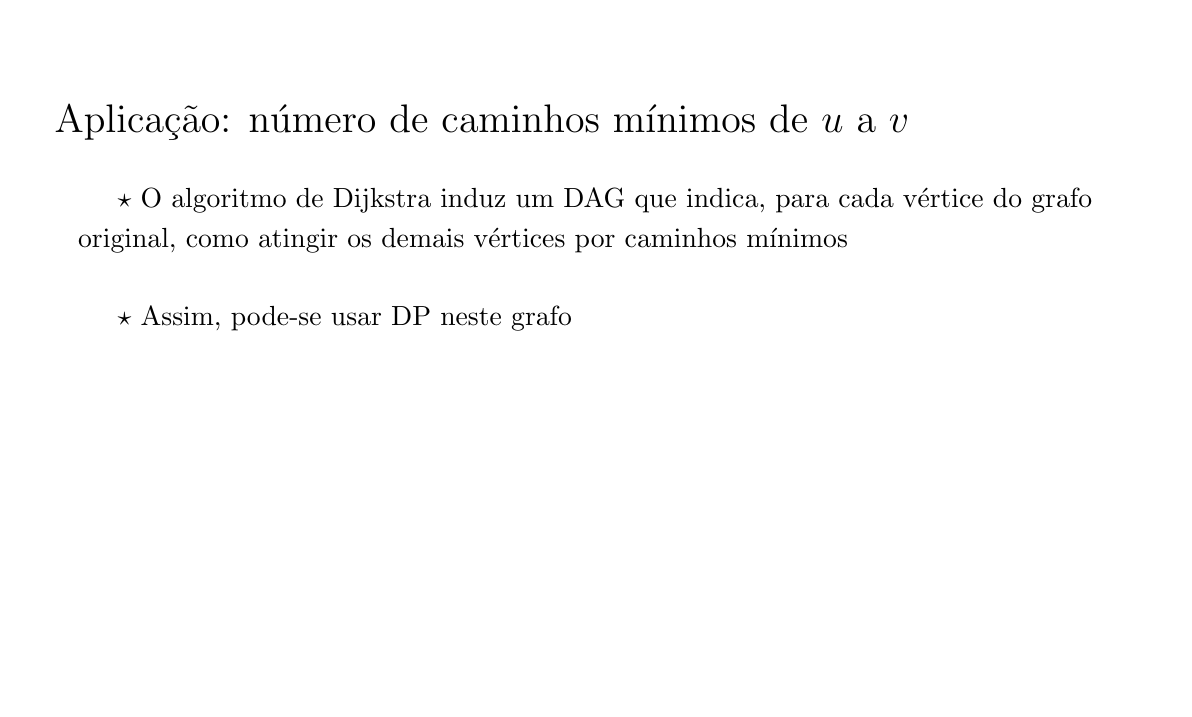
\begin{tikzpicture}
\node[draw,opacity=0] at (0, 0) {x};
\node[draw,opacity=0] at (14, 8) {x};

	\node[anchor=west] (title) at (0.0, 7.0) { \Large \bbbold{Aplicação: número de caminhos mínimos de $u$ a $v$} };

	\node[anchor=west] (a) at (0.8, 6.0) { $\star$ \bbtext{O algoritmo de Dijkstra induz um DAG que indica, para cada vértice do grafo} };

	\node[anchor=west] (a1) at (0.3, 5.5) { \bbtext{original, como atingir os demais vértices por caminhos mínimos} };


	\node[anchor=west] (b) at (0.8, 4.5) { $\star$ \bbtext{Assim, pode-se usar DP neste grafo} };

\end{tikzpicture}
\end{frame}
\begin{frame}[plain,t]
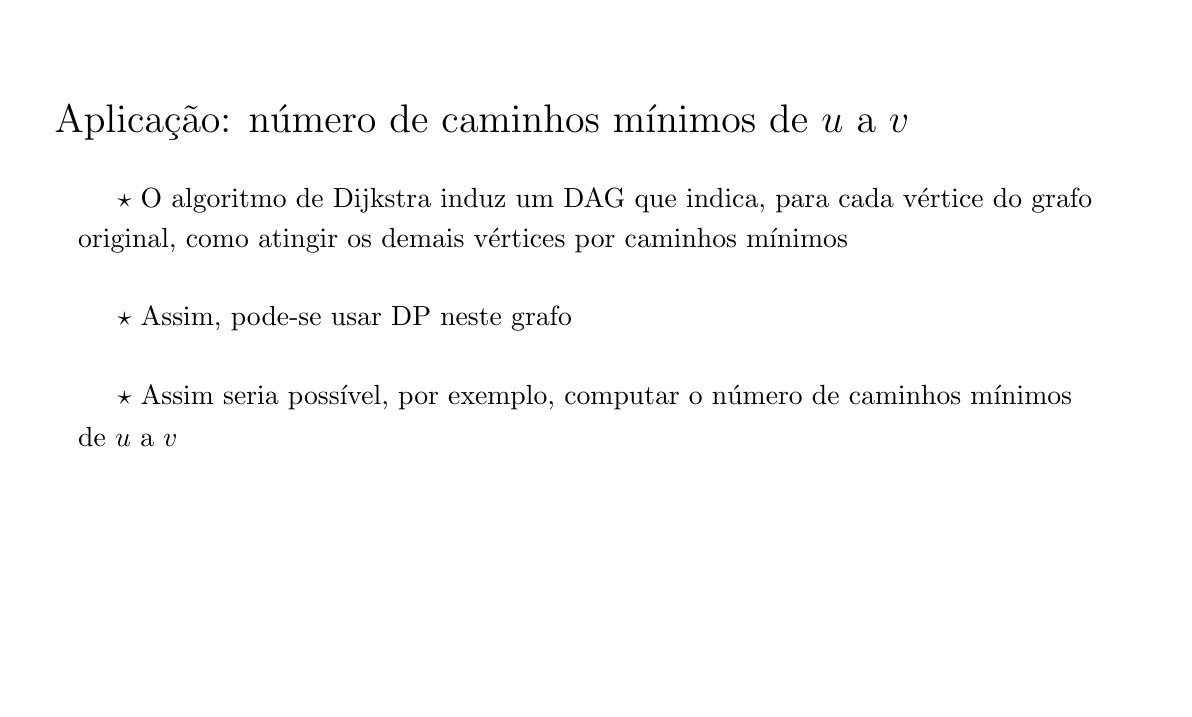
\begin{tikzpicture}
\node[draw,opacity=0] at (0, 0) {x};
\node[draw,opacity=0] at (14, 8) {x};

	\node[anchor=west] (title) at (0.0, 7.0) { \Large \bbbold{Aplicação: número de caminhos mínimos de $u$ a $v$} };

	\node[anchor=west] (a) at (0.8, 6.0) { $\star$ \bbtext{O algoritmo de Dijkstra induz um DAG que indica, para cada vértice do grafo} };

	\node[anchor=west] (a1) at (0.3, 5.5) { \bbtext{original, como atingir os demais vértices por caminhos mínimos} };


	\node[anchor=west] (b) at (0.8, 4.5) { $\star$ \bbtext{Assim, pode-se usar DP neste grafo} };


	\node[anchor=west] (c) at (0.8, 3.5) { $\star$ \bbtext{Assim seria possível, por exemplo, computar o número de caminhos mínimos} };

	\node[anchor=west] (c1) at (0.3, 3.0) { \bbtext{de $u$ a $v$} };

\end{tikzpicture}
\end{frame}
\begin{frame}[plain,t]
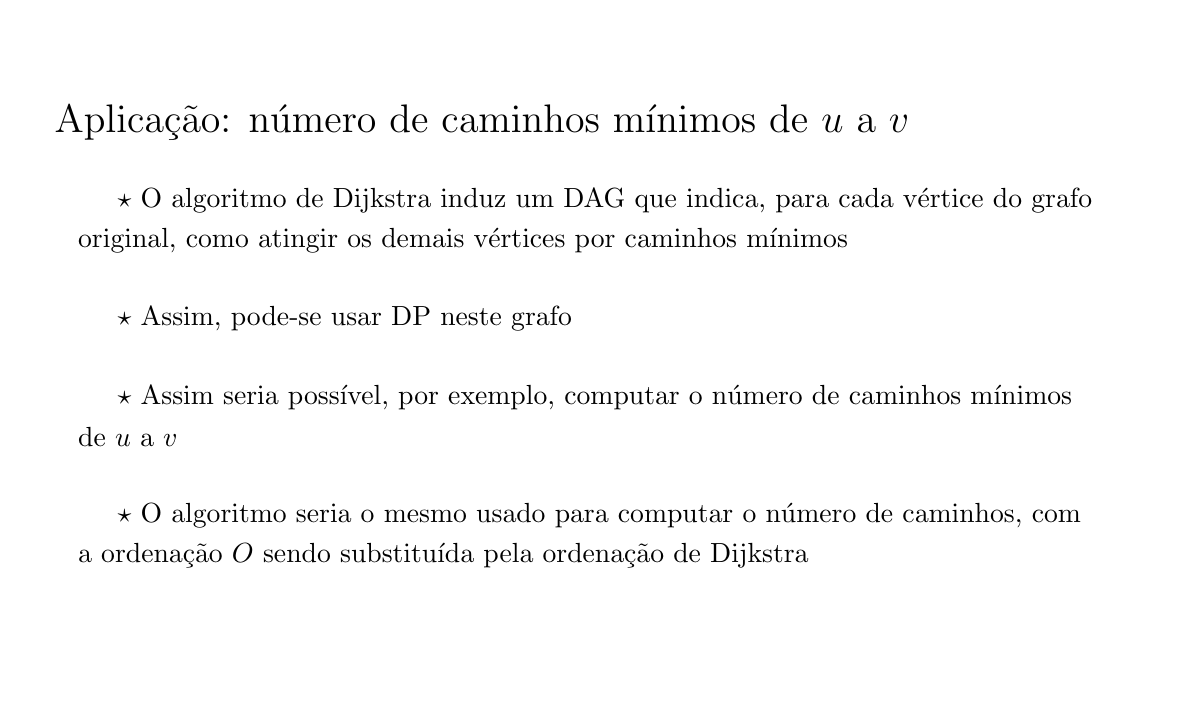
\begin{tikzpicture}
\node[draw,opacity=0] at (0, 0) {x};
\node[draw,opacity=0] at (14, 8) {x};

	\node[anchor=west] (title) at (0.0, 7.0) { \Large \bbbold{Aplicação: número de caminhos mínimos de $u$ a $v$} };

	\node[anchor=west] (a) at (0.8, 6.0) { $\star$ \bbtext{O algoritmo de Dijkstra induz um DAG que indica, para cada vértice do grafo} };

	\node[anchor=west] (a1) at (0.3, 5.5) { \bbtext{original, como atingir os demais vértices por caminhos mínimos} };


	\node[anchor=west] (b) at (0.8, 4.5) { $\star$ \bbtext{Assim, pode-se usar DP neste grafo} };


	\node[anchor=west] (c) at (0.8, 3.5) { $\star$ \bbtext{Assim seria possível, por exemplo, computar o número de caminhos mínimos} };

	\node[anchor=west] (c1) at (0.3, 3.0) { \bbtext{de $u$ a $v$} };


	\node[anchor=west] (d) at (0.8, 2.0) { $\star$ \bbtext{O algoritmo seria o mesmo usado para computar o número de caminhos, com} };

	\node[anchor=west] (d1) at (0.3, 1.5) { \bbtext{a ordenação $O$ sendo substituída pela ordenação de Dijkstra} };

\end{tikzpicture}
\end{frame}
\begin{frame}[plain,t]
\begin{tikzpicture}
\node[draw,opacity=0] at (0, 0) {x};
\node[draw,opacity=0] at (14, 8) {x};

	\node[very thick,draw,circle] (node1) at (1.0, 5.0) { \bbtext{1} };

	\node[very thick,draw,circle] (node2) at (3.0, 7.0) { \bbtext{2} };

	\node[very thick,draw,circle] (node3) at (3.0, 5.0) { \bbtext{3} };

	\node[very thick,draw,circle] (node4) at (3.0, 3.0) { \bbtext{4} };

	\node[very thick,draw,circle] (node5) at (5.0, 5.0) { \bbtext{5} };

	\draw[thick,-latex](node1) to node[above left] { \footnotesize \bbinfo{3} } (node2);

	\draw[thick,-latex](node1) to node[above] { \footnotesize \bbinfo{2} } (node3);

	\draw[thick,-latex](node1) to node[below left] { \footnotesize \bbinfo{5} } (node4);

	\draw[thick,-latex](node3) to node[right] { \footnotesize \bbinfo{1} } (node2);

	\draw[thick,-latex](node3) to node[right] { \footnotesize \bbinfo{2} } (node4);

	\draw[thick,-latex](node2) to node[above right] { \footnotesize \bbinfo{3} } (node5);

	\draw[thick,-latex](node3) to node[above] { \footnotesize \bbinfo{5} } (node5);

	\draw[thick,-latex](node4) to node[below right] { \footnotesize \bbinfo{2} } (node5);

	\draw[thick] (1.0, 0.0) grid  (6.0, 1.0);

	\node[anchor=east] (dist) at (1.0, 0.5) { $d_1(x) = $ };

	\node[] (d1) at (1.5, 1.4) { \bbtext{1} };

	\node[] (d2) at (2.5, 1.4) { \bbtext{2} };

	\node[] (d3) at (3.5, 1.4) { \bbtext{3} };

	\node[] (d4) at (4.5, 1.4) { \bbtext{4} };

	\node[] (d5) at (5.5, 1.4) { \bbtext{5} };

	\node[] (dv1) at (1.5, 0.5) { \bbtext{-} };

	\node[] (dv2) at (2.5, 0.5) { \bbtext{-} };

	\node[] (dv3) at (3.5, 0.5) { \bbtext{-} };

	\node[] (dv4) at (4.5, 0.5) { \bbtext{-} };

	\node[] (dv5) at (5.5, 0.5) { \bbtext{-} };

\end{tikzpicture}
\end{frame}
\begin{frame}[plain,t]
\begin{tikzpicture}
\node[draw,opacity=0] at (0, 0) {x};
\node[draw,opacity=0] at (14, 8) {x};

	\node[very thick,draw,circle,fill=BBGreen] (node1) at (1.0, 5.0) { \bbtext{1} };

	\node[very thick,draw,circle] (node2) at (3.0, 7.0) { \bbtext{2} };

	\node[very thick,draw,circle] (node3) at (3.0, 5.0) { \bbtext{3} };

	\node[very thick,draw,circle] (node4) at (3.0, 3.0) { \bbtext{4} };

	\node[very thick,draw,circle] (node5) at (5.0, 5.0) { \bbtext{5} };

	\draw[thick,-latex](node1) to node[above left] { \footnotesize \bbinfo{3} } (node2);

	\draw[thick,-latex](node1) to node[above] { \footnotesize \bbinfo{2} } (node3);

	\draw[thick,-latex](node1) to node[below left] { \footnotesize \bbinfo{5} } (node4);

	\draw[thick,-latex](node3) to node[right] { \footnotesize \bbinfo{1} } (node2);

	\draw[thick,-latex](node3) to node[right] { \footnotesize \bbinfo{2} } (node4);

	\draw[thick,-latex](node2) to node[above right] { \footnotesize \bbinfo{3} } (node5);

	\draw[thick,-latex](node3) to node[above] { \footnotesize \bbinfo{5} } (node5);

	\draw[thick,-latex](node4) to node[below right] { \footnotesize \bbinfo{2} } (node5);

	\draw[thick] (1.0, 0.0) grid  (6.0, 1.0);

	\node[anchor=east] (dist) at (1.0, 0.5) { $d_1(x) = $ };

	\node[] (d1) at (1.5, 1.4) { \bbtext{1} };

	\node[] (d2) at (2.5, 1.4) { \bbtext{2} };

	\node[] (d3) at (3.5, 1.4) { \bbtext{3} };

	\node[] (d4) at (4.5, 1.4) { \bbtext{4} };

	\node[] (d5) at (5.5, 1.4) { \bbtext{5} };

	\node[] (dv1) at (1.5, 0.5) { $\mathbf{0}$ };

	\node[] (dv2) at (2.5, 0.5) { \bbtext{-} };

	\node[] (dv3) at (3.5, 0.5) { \bbtext{-} };

	\node[] (dv4) at (4.5, 0.5) { \bbtext{-} };

	\node[] (dv5) at (5.5, 0.5) { \bbtext{-} };



\end{tikzpicture}
\end{frame}
\begin{frame}[plain,t]
\begin{tikzpicture}
\node[draw,opacity=0] at (0, 0) {x};
\node[draw,opacity=0] at (14, 8) {x};

	\node[very thick,draw,circle,fill=BBGreen] (node1) at (1.0, 5.0) { \bbtext{1} };

	\node[very thick,draw,circle] (node2) at (3.0, 7.0) { \bbtext{2} };

	\node[very thick,draw,circle] (node3) at (3.0, 5.0) { \bbtext{3} };

	\node[very thick,draw,circle] (node4) at (3.0, 3.0) { \bbtext{4} };

	\node[very thick,draw,circle] (node5) at (5.0, 5.0) { \bbtext{5} };

	\draw[thick,-latex](node1) to node[above left] { \footnotesize \bbinfo{3} } (node2);

	\draw[thick,-latex](node1) to node[above] { \footnotesize \bbinfo{2} } (node3);

	\draw[thick,-latex](node1) to node[below left] { \footnotesize \bbinfo{5} } (node4);

	\draw[thick,-latex](node3) to node[right] { \footnotesize \bbinfo{1} } (node2);

	\draw[thick,-latex](node3) to node[right] { \footnotesize \bbinfo{2} } (node4);

	\draw[thick,-latex](node2) to node[above right] { \footnotesize \bbinfo{3} } (node5);

	\draw[thick,-latex](node3) to node[above] { \footnotesize \bbinfo{5} } (node5);

	\draw[thick,-latex](node4) to node[below right] { \footnotesize \bbinfo{2} } (node5);

	\draw[thick] (1.0, 0.0) grid  (6.0, 1.0);

	\node[anchor=east] (dist) at (1.0, 0.5) { $d_1(x) = $ };

	\node[] (d1) at (1.5, 1.4) { \bbtext{1} };

	\node[] (d2) at (2.5, 1.4) { \bbtext{2} };

	\node[] (d3) at (3.5, 1.4) { \bbtext{3} };

	\node[] (d4) at (4.5, 1.4) { \bbtext{4} };

	\node[] (d5) at (5.5, 1.4) { \bbtext{5} };

	\node[] (dv1) at (1.5, 0.5) { ${0}$ };

	\node[] (dv2) at (2.5, 0.5) { \bbtext{-} };

	\node[] (dv3) at (3.5, 0.5) { \bbtext{-} };

	\node[] (dv4) at (4.5, 0.5) { \bbtext{-} };

	\node[] (dv5) at (5.5, 0.5) { \bbtext{-} };





	\node[very thick,draw,circle] (n1) at (8.0, 5.0) { \textcolor{BBEmerald}{\textbf{1}}$^1$ };

\end{tikzpicture}
\end{frame}
\begin{frame}[plain,t]
\begin{tikzpicture}
\node[draw,opacity=0] at (0, 0) {x};
\node[draw,opacity=0] at (14, 8) {x};

	\node[very thick,draw,circle,fill=BBGreen] (node1) at (1.0, 5.0) { \bbtext{1} };

	\node[very thick,draw,circle] (node2) at (3.0, 7.0) { \bbtext{2} };

	\node[very thick,draw,circle] (node3) at (3.0, 5.0) { \bbtext{3} };

	\node[very thick,draw,circle] (node4) at (3.0, 3.0) { \bbtext{4} };

	\node[very thick,draw,circle] (node5) at (5.0, 5.0) { \bbtext{5} };

	\draw[thick,-latex,color=BBCyan](node1) to node[above left] { \footnotesize \bbinfo{3} } (node2);

	\draw[thick,-latex](node1) to node[above] { \footnotesize \bbinfo{2} } (node3);

	\draw[thick,-latex](node1) to node[below left] { \footnotesize \bbinfo{5} } (node4);

	\draw[thick,-latex](node3) to node[right] { \footnotesize \bbinfo{1} } (node2);

	\draw[thick,-latex](node3) to node[right] { \footnotesize \bbinfo{2} } (node4);

	\draw[thick,-latex](node2) to node[above right] { \footnotesize \bbinfo{3} } (node5);

	\draw[thick,-latex](node3) to node[above] { \footnotesize \bbinfo{5} } (node5);

	\draw[thick,-latex](node4) to node[below right] { \footnotesize \bbinfo{2} } (node5);

	\draw[thick] (1.0, 0.0) grid  (6.0, 1.0);

	\node[anchor=east] (dist) at (1.0, 0.5) { $d_1(x) = $ };

	\node[] (d1) at (1.5, 1.4) { \bbtext{1} };

	\node[] (d2) at (2.5, 1.4) { \bbtext{2} };

	\node[] (d3) at (3.5, 1.4) { \bbtext{3} };

	\node[] (d4) at (4.5, 1.4) { \bbtext{4} };

	\node[] (d5) at (5.5, 1.4) { \bbtext{5} };

	\node[] (dv1) at (1.5, 0.5) { ${0}$ };

	\node[] (dv2) at (2.5, 0.5) { $\mathbf{3}$ };

	\node[] (dv3) at (3.5, 0.5) { \bbtext{-} };

	\node[] (dv4) at (4.5, 0.5) { \bbtext{-} };

	\node[] (dv5) at (5.5, 0.5) { \bbtext{-} };





	\node[very thick,draw,circle] (n1) at (8.0, 5.0) { \textcolor{BBEmerald}{\textbf{1}}$^1$ };


\end{tikzpicture}
\end{frame}
\begin{frame}[plain,t]
\begin{tikzpicture}
\node[draw,opacity=0] at (0, 0) {x};
\node[draw,opacity=0] at (14, 8) {x};

	\node[very thick,draw,circle,fill=BBGreen] (node1) at (1.0, 5.0) { \bbtext{1} };

	\node[very thick,draw,circle] (node2) at (3.0, 7.0) { \bbtext{2} };

	\node[very thick,draw,circle] (node3) at (3.0, 5.0) { \bbtext{3} };

	\node[very thick,draw,circle] (node4) at (3.0, 3.0) { \bbtext{4} };

	\node[very thick,draw,circle] (node5) at (5.0, 5.0) { \bbtext{5} };

	\draw[thick,-latex,color=BBBlack](node1) to node[above left] { \footnotesize \bbinfo{3} } (node2);

	\draw[thick,-latex,color=BBCyan](node1) to node[above] { \footnotesize \bbinfo{2} } (node3);

	\draw[thick,-latex](node1) to node[below left] { \footnotesize \bbinfo{5} } (node4);

	\draw[thick,-latex](node3) to node[right] { \footnotesize \bbinfo{1} } (node2);

	\draw[thick,-latex](node3) to node[right] { \footnotesize \bbinfo{2} } (node4);

	\draw[thick,-latex](node2) to node[above right] { \footnotesize \bbinfo{3} } (node5);

	\draw[thick,-latex](node3) to node[above] { \footnotesize \bbinfo{5} } (node5);

	\draw[thick,-latex](node4) to node[below right] { \footnotesize \bbinfo{2} } (node5);

	\draw[thick] (1.0, 0.0) grid  (6.0, 1.0);

	\node[anchor=east] (dist) at (1.0, 0.5) { $d_1(x) = $ };

	\node[] (d1) at (1.5, 1.4) { \bbtext{1} };

	\node[] (d2) at (2.5, 1.4) { \bbtext{2} };

	\node[] (d3) at (3.5, 1.4) { \bbtext{3} };

	\node[] (d4) at (4.5, 1.4) { \bbtext{4} };

	\node[] (d5) at (5.5, 1.4) { \bbtext{5} };

	\node[] (dv1) at (1.5, 0.5) { ${0}$ };

	\node[] (dv2) at (2.5, 0.5) { ${3}$ };

	\node[] (dv3) at (3.5, 0.5) { $\mathbf{2}$ };

	\node[] (dv4) at (4.5, 0.5) { \bbtext{-} };

	\node[] (dv5) at (5.5, 0.5) { \bbtext{-} };





	\node[very thick,draw,circle] (n1) at (8.0, 5.0) { \textcolor{BBEmerald}{\textbf{1}}$^1$ };




\end{tikzpicture}
\end{frame}
\begin{frame}[plain,t]
\begin{tikzpicture}
\node[draw,opacity=0] at (0, 0) {x};
\node[draw,opacity=0] at (14, 8) {x};

	\node[very thick,draw,circle,fill=BBGreen] (node1) at (1.0, 5.0) { \bbtext{1} };

	\node[very thick,draw,circle] (node2) at (3.0, 7.0) { \bbtext{2} };

	\node[very thick,draw,circle] (node3) at (3.0, 5.0) { \bbtext{3} };

	\node[very thick,draw,circle] (node4) at (3.0, 3.0) { \bbtext{4} };

	\node[very thick,draw,circle] (node5) at (5.0, 5.0) { \bbtext{5} };

	\draw[thick,-latex,color=BBBlack](node1) to node[above left] { \footnotesize \bbinfo{3} } (node2);

	\draw[thick,-latex,color=BBBlack](node1) to node[above] { \footnotesize \bbinfo{2} } (node3);

	\draw[thick,-latex,color=BBCyan](node1) to node[below left] { \footnotesize \bbinfo{5} } (node4);

	\draw[thick,-latex](node3) to node[right] { \footnotesize \bbinfo{1} } (node2);

	\draw[thick,-latex](node3) to node[right] { \footnotesize \bbinfo{2} } (node4);

	\draw[thick,-latex](node2) to node[above right] { \footnotesize \bbinfo{3} } (node5);

	\draw[thick,-latex](node3) to node[above] { \footnotesize \bbinfo{5} } (node5);

	\draw[thick,-latex](node4) to node[below right] { \footnotesize \bbinfo{2} } (node5);

	\draw[thick] (1.0, 0.0) grid  (6.0, 1.0);

	\node[anchor=east] (dist) at (1.0, 0.5) { $d_1(x) = $ };

	\node[] (d1) at (1.5, 1.4) { \bbtext{1} };

	\node[] (d2) at (2.5, 1.4) { \bbtext{2} };

	\node[] (d3) at (3.5, 1.4) { \bbtext{3} };

	\node[] (d4) at (4.5, 1.4) { \bbtext{4} };

	\node[] (d5) at (5.5, 1.4) { \bbtext{5} };

	\node[] (dv1) at (1.5, 0.5) { ${0}$ };

	\node[] (dv2) at (2.5, 0.5) { ${3}$ };

	\node[] (dv3) at (3.5, 0.5) { ${2}$ };

	\node[] (dv4) at (4.5, 0.5) { $\mathbf{5}$ };

	\node[] (dv5) at (5.5, 0.5) { \bbtext{-} };





	\node[very thick,draw,circle] (n1) at (8.0, 5.0) { \textcolor{BBEmerald}{\textbf{1}}$^1$ };






\end{tikzpicture}
\end{frame}
\begin{frame}[plain,t]
\begin{tikzpicture}
\node[draw,opacity=0] at (0, 0) {x};
\node[draw,opacity=0] at (14, 8) {x};

	\node[very thick,draw,circle,fill=BBCyan] (node1) at (1.0, 5.0) { \bbtext{1} };

	\node[very thick,draw,circle] (node2) at (3.0, 7.0) { \bbtext{2} };

	\node[very thick,draw,circle] (node3) at (3.0, 5.0) { \bbtext{3} };

	\node[very thick,draw,circle] (node4) at (3.0, 3.0) { \bbtext{4} };

	\node[very thick,draw,circle] (node5) at (5.0, 5.0) { \bbtext{5} };

	\draw[thick,-latex,color=BBBlack](node1) to node[above left] { \footnotesize \bbinfo{3} } (node2);

	\draw[thick,-latex,color=BBBlack](node1) to node[above] { \footnotesize \bbinfo{2} } (node3);

	\draw[thick,-latex,color=BBBlack](node1) to node[below left] { \footnotesize \bbinfo{5} } (node4);

	\draw[thick,-latex](node3) to node[right] { \footnotesize \bbinfo{1} } (node2);

	\draw[thick,-latex](node3) to node[right] { \footnotesize \bbinfo{2} } (node4);

	\draw[thick,-latex](node2) to node[above right] { \footnotesize \bbinfo{3} } (node5);

	\draw[thick,-latex](node3) to node[above] { \footnotesize \bbinfo{5} } (node5);

	\draw[thick,-latex](node4) to node[below right] { \footnotesize \bbinfo{2} } (node5);

	\draw[thick] (1.0, 0.0) grid  (6.0, 1.0);

	\node[anchor=east] (dist) at (1.0, 0.5) { $d_1(x) = $ };

	\node[] (d1) at (1.5, 1.4) { \bbtext{1} };

	\node[] (d2) at (2.5, 1.4) { \bbtext{2} };

	\node[] (d3) at (3.5, 1.4) { \bbtext{3} };

	\node[] (d4) at (4.5, 1.4) { \bbtext{4} };

	\node[] (d5) at (5.5, 1.4) { \bbtext{5} };

	\node[] (dv1) at (1.5, 0.5) { ${0}$ };

	\node[] (dv2) at (2.5, 0.5) { ${3}$ };

	\node[] (dv3) at (3.5, 0.5) { ${2}$ };

	\node[] (dv4) at (4.5, 0.5) { ${5}$ };

	\node[] (dv5) at (5.5, 0.5) { \bbtext{-} };





	\node[very thick,draw,circle] (n1) at (8.0, 5.0) { \textcolor{BBEmerald}{\textbf{1}}$^1$ };








\end{tikzpicture}
\end{frame}
\begin{frame}[plain,t]
\begin{tikzpicture}
\node[draw,opacity=0] at (0, 0) {x};
\node[draw,opacity=0] at (14, 8) {x};

	\node[very thick,draw,circle,fill=BBCyan] (node1) at (1.0, 5.0) { \bbtext{1} };

	\node[very thick,draw,circle] (node2) at (3.0, 7.0) { \bbtext{2} };

	\node[very thick,draw,circle,fill=BBGreen] (node3) at (3.0, 5.0) { \bbtext{3} };

	\node[very thick,draw,circle] (node4) at (3.0, 3.0) { \bbtext{4} };

	\node[very thick,draw,circle] (node5) at (5.0, 5.0) { \bbtext{5} };

	\draw[thick,-latex,color=BBBlack](node1) to node[above left] { \footnotesize \bbinfo{3} } (node2);

	\draw[thick,-latex,color=BBBlack](node1) to node[above] { \footnotesize \bbinfo{2} } (node3);

	\draw[thick,-latex,color=BBBlack](node1) to node[below left] { \footnotesize \bbinfo{5} } (node4);

	\draw[thick,-latex](node3) to node[right] { \footnotesize \bbinfo{1} } (node2);

	\draw[thick,-latex](node3) to node[right] { \footnotesize \bbinfo{2} } (node4);

	\draw[thick,-latex](node2) to node[above right] { \footnotesize \bbinfo{3} } (node5);

	\draw[thick,-latex](node3) to node[above] { \footnotesize \bbinfo{5} } (node5);

	\draw[thick,-latex](node4) to node[below right] { \footnotesize \bbinfo{2} } (node5);

	\draw[thick] (1.0, 0.0) grid  (6.0, 1.0);

	\node[anchor=east] (dist) at (1.0, 0.5) { $d_1(x) = $ };

	\node[] (d1) at (1.5, 1.4) { \bbtext{1} };

	\node[] (d2) at (2.5, 1.4) { \bbtext{2} };

	\node[] (d3) at (3.5, 1.4) { \bbtext{3} };

	\node[] (d4) at (4.5, 1.4) { \bbtext{4} };

	\node[] (d5) at (5.5, 1.4) { \bbtext{5} };

	\node[] (dv1) at (1.5, 0.5) { ${0}$ };

	\node[] (dv2) at (2.5, 0.5) { ${3}$ };

	\node[] (dv3) at (3.5, 0.5) { ${2}$ };

	\node[] (dv4) at (4.5, 0.5) { ${5}$ };

	\node[] (dv5) at (5.5, 0.5) { \bbtext{-} };





	\node[very thick,draw,circle] (n1) at (8.0, 5.0) { \textcolor{BBEmerald}{\textbf{1}}$^1$ };










\end{tikzpicture}
\end{frame}
\begin{frame}[plain,t]
\begin{tikzpicture}
\node[draw,opacity=0] at (0, 0) {x};
\node[draw,opacity=0] at (14, 8) {x};

	\node[very thick,draw,circle,fill=BBCyan] (node1) at (1.0, 5.0) { \bbtext{1} };

	\node[very thick,draw,circle] (node2) at (3.0, 7.0) { \bbtext{2} };

	\node[very thick,draw,circle,fill=BBGreen] (node3) at (3.0, 5.0) { \bbtext{3} };

	\node[very thick,draw,circle] (node4) at (3.0, 3.0) { \bbtext{4} };

	\node[very thick,draw,circle] (node5) at (5.0, 5.0) { \bbtext{5} };

	\draw[thick,-latex,color=BBBlack](node1) to node[above left] { \footnotesize \bbinfo{3} } (node2);

	\draw[thick,-latex,color=BBBlack](node1) to node[above] { \footnotesize \bbinfo{2} } (node3);

	\draw[thick,-latex,color=BBBlack](node1) to node[below left] { \footnotesize \bbinfo{5} } (node4);

	\draw[thick,-latex](node3) to node[right] { \footnotesize \bbinfo{1} } (node2);

	\draw[thick,-latex](node3) to node[right] { \footnotesize \bbinfo{2} } (node4);

	\draw[thick,-latex](node2) to node[above right] { \footnotesize \bbinfo{3} } (node5);

	\draw[thick,-latex](node3) to node[above] { \footnotesize \bbinfo{5} } (node5);

	\draw[thick,-latex](node4) to node[below right] { \footnotesize \bbinfo{2} } (node5);

	\draw[thick] (1.0, 0.0) grid  (6.0, 1.0);

	\node[anchor=east] (dist) at (1.0, 0.5) { $d_1(x) = $ };

	\node[] (d1) at (1.5, 1.4) { \bbtext{1} };

	\node[] (d2) at (2.5, 1.4) { \bbtext{2} };

	\node[] (d3) at (3.5, 1.4) { \bbtext{3} };

	\node[] (d4) at (4.5, 1.4) { \bbtext{4} };

	\node[] (d5) at (5.5, 1.4) { \bbtext{5} };

	\node[] (dv1) at (1.5, 0.5) { ${0}$ };

	\node[] (dv2) at (2.5, 0.5) { ${3}$ };

	\node[] (dv3) at (3.5, 0.5) { ${2}$ };

	\node[] (dv4) at (4.5, 0.5) { ${5}$ };

	\node[] (dv5) at (5.5, 0.5) { \bbtext{-} };





	\node[very thick,draw,circle] (n1) at (8.0, 5.0) { \textcolor{BBEmerald}{\textbf{1}}$^1$ };










	\node[very thick,draw,circle] (n3) at (10.0, 5.0) { \textcolor{BBEmerald}{\textbf{3}}$^2$ };

	\draw[thick,dashed,-latex](n1) to (n3);

\end{tikzpicture}
\end{frame}
\begin{frame}[plain,t]
\begin{tikzpicture}
\node[draw,opacity=0] at (0, 0) {x};
\node[draw,opacity=0] at (14, 8) {x};

	\node[very thick,draw,circle,fill=BBCyan] (node1) at (1.0, 5.0) { \bbtext{1} };

	\node[very thick,draw,circle] (node2) at (3.0, 7.0) { \bbtext{2} };

	\node[very thick,draw,circle,fill=BBGreen] (node3) at (3.0, 5.0) { \bbtext{3} };

	\node[very thick,draw,circle] (node4) at (3.0, 3.0) { \bbtext{4} };

	\node[very thick,draw,circle] (node5) at (5.0, 5.0) { \bbtext{5} };

	\draw[thick,-latex,color=BBBlack](node1) to node[above left] { \footnotesize \bbinfo{3} } (node2);

	\draw[thick,-latex,color=BBBlack](node1) to node[above] { \footnotesize \bbinfo{2} } (node3);

	\draw[thick,-latex,color=BBBlack](node1) to node[below left] { \footnotesize \bbinfo{5} } (node4);

	\draw[thick,-latex,color=BBCyan](node3) to node[right] { \footnotesize \bbinfo{1} } (node2);

	\draw[thick,-latex](node3) to node[right] { \footnotesize \bbinfo{2} } (node4);

	\draw[thick,-latex](node2) to node[above right] { \footnotesize \bbinfo{3} } (node5);

	\draw[thick,-latex](node3) to node[above] { \footnotesize \bbinfo{5} } (node5);

	\draw[thick,-latex](node4) to node[below right] { \footnotesize \bbinfo{2} } (node5);

	\draw[thick] (1.0, 0.0) grid  (6.0, 1.0);

	\node[anchor=east] (dist) at (1.0, 0.5) { $d_1(x) = $ };

	\node[] (d1) at (1.5, 1.4) { \bbtext{1} };

	\node[] (d2) at (2.5, 1.4) { \bbtext{2} };

	\node[] (d3) at (3.5, 1.4) { \bbtext{3} };

	\node[] (d4) at (4.5, 1.4) { \bbtext{4} };

	\node[] (d5) at (5.5, 1.4) { \bbtext{5} };

	\node[] (dv1) at (1.5, 0.5) { ${0}$ };

	\node[] (dv2) at (2.5, 0.5) { ${3}$ };

	\node[] (dv3) at (3.5, 0.5) { ${2}$ };

	\node[] (dv4) at (4.5, 0.5) { ${5}$ };

	\node[] (dv5) at (5.5, 0.5) { \bbtext{-} };





	\node[very thick,draw,circle] (n1) at (8.0, 5.0) { \textcolor{BBEmerald}{\textbf{1}}$^1$ };










	\node[very thick,draw,circle] (n3) at (10.0, 5.0) { \textcolor{BBEmerald}{\textbf{3}}$^2$ };

	\draw[thick,dashed,-latex](n1) to (n3);


\end{tikzpicture}
\end{frame}
\begin{frame}[plain,t]
\begin{tikzpicture}
\node[draw,opacity=0] at (0, 0) {x};
\node[draw,opacity=0] at (14, 8) {x};

	\node[very thick,draw,circle,fill=BBCyan] (node1) at (1.0, 5.0) { \bbtext{1} };

	\node[very thick,draw,circle] (node2) at (3.0, 7.0) { \bbtext{2} };

	\node[very thick,draw,circle,fill=BBGreen] (node3) at (3.0, 5.0) { \bbtext{3} };

	\node[very thick,draw,circle] (node4) at (3.0, 3.0) { \bbtext{4} };

	\node[very thick,draw,circle] (node5) at (5.0, 5.0) { \bbtext{5} };

	\draw[thick,-latex,color=BBBlack](node1) to node[above left] { \footnotesize \bbinfo{3} } (node2);

	\draw[thick,-latex,color=BBBlack](node1) to node[above] { \footnotesize \bbinfo{2} } (node3);

	\draw[thick,-latex,color=BBBlack](node1) to node[below left] { \footnotesize \bbinfo{5} } (node4);

	\draw[thick,-latex,color=BBBlack](node3) to node[right] { \footnotesize \bbinfo{1} } (node2);

	\draw[thick,-latex,color=BBCyan](node3) to node[right] { \footnotesize \bbinfo{2} } (node4);

	\draw[thick,-latex](node2) to node[above right] { \footnotesize \bbinfo{3} } (node5);

	\draw[thick,-latex](node3) to node[above] { \footnotesize \bbinfo{5} } (node5);

	\draw[thick,-latex](node4) to node[below right] { \footnotesize \bbinfo{2} } (node5);

	\draw[thick] (1.0, 0.0) grid  (6.0, 1.0);

	\node[anchor=east] (dist) at (1.0, 0.5) { $d_1(x) = $ };

	\node[] (d1) at (1.5, 1.4) { \bbtext{1} };

	\node[] (d2) at (2.5, 1.4) { \bbtext{2} };

	\node[] (d3) at (3.5, 1.4) { \bbtext{3} };

	\node[] (d4) at (4.5, 1.4) { \bbtext{4} };

	\node[] (d5) at (5.5, 1.4) { \bbtext{5} };

	\node[] (dv1) at (1.5, 0.5) { ${0}$ };

	\node[] (dv2) at (2.5, 0.5) { ${3}$ };

	\node[] (dv3) at (3.5, 0.5) { ${2}$ };

	\node[] (dv4) at (4.5, 0.5) { $\mathbf{4}$ };

	\node[] (dv5) at (5.5, 0.5) { \bbtext{-} };





	\node[very thick,draw,circle] (n1) at (8.0, 5.0) { \textcolor{BBEmerald}{\textbf{1}}$^1$ };










	\node[very thick,draw,circle] (n3) at (10.0, 5.0) { \textcolor{BBEmerald}{\textbf{3}}$^2$ };

	\draw[thick,dashed,-latex](n1) to (n3);



\end{tikzpicture}
\end{frame}
\begin{frame}[plain,t]
\begin{tikzpicture}
\node[draw,opacity=0] at (0, 0) {x};
\node[draw,opacity=0] at (14, 8) {x};

	\node[very thick,draw,circle,fill=BBCyan] (node1) at (1.0, 5.0) { \bbtext{1} };

	\node[very thick,draw,circle] (node2) at (3.0, 7.0) { \bbtext{2} };

	\node[very thick,draw,circle,fill=BBGreen] (node3) at (3.0, 5.0) { \bbtext{3} };

	\node[very thick,draw,circle] (node4) at (3.0, 3.0) { \bbtext{4} };

	\node[very thick,draw,circle] (node5) at (5.0, 5.0) { \bbtext{5} };

	\draw[thick,-latex,color=BBBlack](node1) to node[above left] { \footnotesize \bbinfo{3} } (node2);

	\draw[thick,-latex,color=BBBlack](node1) to node[above] { \footnotesize \bbinfo{2} } (node3);

	\draw[thick,-latex,color=BBBlack](node1) to node[below left] { \footnotesize \bbinfo{5} } (node4);

	\draw[thick,-latex,color=BBBlack](node3) to node[right] { \footnotesize \bbinfo{1} } (node2);

	\draw[thick,-latex,color=BBBlack](node3) to node[right] { \footnotesize \bbinfo{2} } (node4);

	\draw[thick,-latex](node2) to node[above right] { \footnotesize \bbinfo{3} } (node5);

	\draw[thick,-latex,color=BBCyan](node3) to node[above] { \footnotesize \bbinfo{5} } (node5);

	\draw[thick,-latex](node4) to node[below right] { \footnotesize \bbinfo{2} } (node5);

	\draw[thick] (1.0, 0.0) grid  (6.0, 1.0);

	\node[anchor=east] (dist) at (1.0, 0.5) { $d_1(x) = $ };

	\node[] (d1) at (1.5, 1.4) { \bbtext{1} };

	\node[] (d2) at (2.5, 1.4) { \bbtext{2} };

	\node[] (d3) at (3.5, 1.4) { \bbtext{3} };

	\node[] (d4) at (4.5, 1.4) { \bbtext{4} };

	\node[] (d5) at (5.5, 1.4) { \bbtext{5} };

	\node[] (dv1) at (1.5, 0.5) { ${0}$ };

	\node[] (dv2) at (2.5, 0.5) { ${3}$ };

	\node[] (dv3) at (3.5, 0.5) { ${2}$ };

	\node[] (dv4) at (4.5, 0.5) { ${4}$ };

	\node[] (dv5) at (5.5, 0.5) { $\mathbf{7}$ };





	\node[very thick,draw,circle] (n1) at (8.0, 5.0) { \textcolor{BBEmerald}{\textbf{1}}$^1$ };










	\node[very thick,draw,circle] (n3) at (10.0, 5.0) { \textcolor{BBEmerald}{\textbf{3}}$^2$ };

	\draw[thick,dashed,-latex](n1) to (n3);





\end{tikzpicture}
\end{frame}
\begin{frame}[plain,t]
\begin{tikzpicture}
\node[draw,opacity=0] at (0, 0) {x};
\node[draw,opacity=0] at (14, 8) {x};

	\node[very thick,draw,circle,fill=BBCyan] (node1) at (1.0, 5.0) { \bbtext{1} };

	\node[very thick,draw,circle] (node2) at (3.0, 7.0) { \bbtext{2} };

	\node[very thick,draw,circle,fill=BBCyan] (node3) at (3.0, 5.0) { \bbtext{3} };

	\node[very thick,draw,circle] (node4) at (3.0, 3.0) { \bbtext{4} };

	\node[very thick,draw,circle] (node5) at (5.0, 5.0) { \bbtext{5} };

	\draw[thick,-latex,color=BBBlack](node1) to node[above left] { \footnotesize \bbinfo{3} } (node2);

	\draw[thick,-latex,color=BBBlack](node1) to node[above] { \footnotesize \bbinfo{2} } (node3);

	\draw[thick,-latex,color=BBBlack](node1) to node[below left] { \footnotesize \bbinfo{5} } (node4);

	\draw[thick,-latex,color=BBBlack](node3) to node[right] { \footnotesize \bbinfo{1} } (node2);

	\draw[thick,-latex,color=BBBlack](node3) to node[right] { \footnotesize \bbinfo{2} } (node4);

	\draw[thick,-latex](node2) to node[above right] { \footnotesize \bbinfo{3} } (node5);

	\draw[thick,-latex,color=BBBlack](node3) to node[above] { \footnotesize \bbinfo{5} } (node5);

	\draw[thick,-latex](node4) to node[below right] { \footnotesize \bbinfo{2} } (node5);

	\draw[thick] (1.0, 0.0) grid  (6.0, 1.0);

	\node[anchor=east] (dist) at (1.0, 0.5) { $d_1(x) = $ };

	\node[] (d1) at (1.5, 1.4) { \bbtext{1} };

	\node[] (d2) at (2.5, 1.4) { \bbtext{2} };

	\node[] (d3) at (3.5, 1.4) { \bbtext{3} };

	\node[] (d4) at (4.5, 1.4) { \bbtext{4} };

	\node[] (d5) at (5.5, 1.4) { \bbtext{5} };

	\node[] (dv1) at (1.5, 0.5) { ${0}$ };

	\node[] (dv2) at (2.5, 0.5) { ${3}$ };

	\node[] (dv3) at (3.5, 0.5) { ${2}$ };

	\node[] (dv4) at (4.5, 0.5) { ${4}$ };

	\node[] (dv5) at (5.5, 0.5) { ${7}$ };





	\node[very thick,draw,circle] (n1) at (8.0, 5.0) { \textcolor{BBEmerald}{\textbf{1}}$^1$ };










	\node[very thick,draw,circle] (n3) at (10.0, 5.0) { \textcolor{BBEmerald}{\textbf{3}}$^2$ };

	\draw[thick,dashed,-latex](n1) to (n3);






\end{tikzpicture}
\end{frame}
\begin{frame}[plain,t]
\begin{tikzpicture}
\node[draw,opacity=0] at (0, 0) {x};
\node[draw,opacity=0] at (14, 8) {x};

	\node[very thick,draw,circle,fill=BBCyan] (node1) at (1.0, 5.0) { \bbtext{1} };

	\node[very thick,draw,circle,fill=BBGreen] (node2) at (3.0, 7.0) { \bbtext{2} };

	\node[very thick,draw,circle,fill=BBCyan] (node3) at (3.0, 5.0) { \bbtext{3} };

	\node[very thick,draw,circle] (node4) at (3.0, 3.0) { \bbtext{4} };

	\node[very thick,draw,circle] (node5) at (5.0, 5.0) { \bbtext{5} };

	\draw[thick,-latex,color=BBBlack](node1) to node[above left] { \footnotesize \bbinfo{3} } (node2);

	\draw[thick,-latex,color=BBBlack](node1) to node[above] { \footnotesize \bbinfo{2} } (node3);

	\draw[thick,-latex,color=BBBlack](node1) to node[below left] { \footnotesize \bbinfo{5} } (node4);

	\draw[thick,-latex,color=BBBlack](node3) to node[right] { \footnotesize \bbinfo{1} } (node2);

	\draw[thick,-latex,color=BBBlack](node3) to node[right] { \footnotesize \bbinfo{2} } (node4);

	\draw[thick,-latex](node2) to node[above right] { \footnotesize \bbinfo{3} } (node5);

	\draw[thick,-latex,color=BBBlack](node3) to node[above] { \footnotesize \bbinfo{5} } (node5);

	\draw[thick,-latex](node4) to node[below right] { \footnotesize \bbinfo{2} } (node5);

	\draw[thick] (1.0, 0.0) grid  (6.0, 1.0);

	\node[anchor=east] (dist) at (1.0, 0.5) { $d_1(x) = $ };

	\node[] (d1) at (1.5, 1.4) { \bbtext{1} };

	\node[] (d2) at (2.5, 1.4) { \bbtext{2} };

	\node[] (d3) at (3.5, 1.4) { \bbtext{3} };

	\node[] (d4) at (4.5, 1.4) { \bbtext{4} };

	\node[] (d5) at (5.5, 1.4) { \bbtext{5} };

	\node[] (dv1) at (1.5, 0.5) { ${0}$ };

	\node[] (dv2) at (2.5, 0.5) { ${3}$ };

	\node[] (dv3) at (3.5, 0.5) { ${2}$ };

	\node[] (dv4) at (4.5, 0.5) { ${4}$ };

	\node[] (dv5) at (5.5, 0.5) { ${7}$ };





	\node[very thick,draw,circle] (n1) at (8.0, 5.0) { \textcolor{BBEmerald}{\textbf{1}}$^1$ };










	\node[very thick,draw,circle] (n3) at (10.0, 5.0) { \textcolor{BBEmerald}{\textbf{3}}$^2$ };

	\draw[thick,dashed,-latex](n1) to (n3);







\end{tikzpicture}
\end{frame}
\begin{frame}[plain,t]
\begin{tikzpicture}
\node[draw,opacity=0] at (0, 0) {x};
\node[draw,opacity=0] at (14, 8) {x};

	\node[very thick,draw,circle,fill=BBCyan] (node1) at (1.0, 5.0) { \bbtext{1} };

	\node[very thick,draw,circle,fill=BBGreen] (node2) at (3.0, 7.0) { \bbtext{2} };

	\node[very thick,draw,circle,fill=BBCyan] (node3) at (3.0, 5.0) { \bbtext{3} };

	\node[very thick,draw,circle] (node4) at (3.0, 3.0) { \bbtext{4} };

	\node[very thick,draw,circle] (node5) at (5.0, 5.0) { \bbtext{5} };

	\draw[thick,-latex,color=BBBlack](node1) to node[above left] { \footnotesize \bbinfo{3} } (node2);

	\draw[thick,-latex,color=BBBlack](node1) to node[above] { \footnotesize \bbinfo{2} } (node3);

	\draw[thick,-latex,color=BBBlack](node1) to node[below left] { \footnotesize \bbinfo{5} } (node4);

	\draw[thick,-latex,color=BBBlack](node3) to node[right] { \footnotesize \bbinfo{1} } (node2);

	\draw[thick,-latex,color=BBBlack](node3) to node[right] { \footnotesize \bbinfo{2} } (node4);

	\draw[thick,-latex](node2) to node[above right] { \footnotesize \bbinfo{3} } (node5);

	\draw[thick,-latex,color=BBBlack](node3) to node[above] { \footnotesize \bbinfo{5} } (node5);

	\draw[thick,-latex](node4) to node[below right] { \footnotesize \bbinfo{2} } (node5);

	\draw[thick] (1.0, 0.0) grid  (6.0, 1.0);

	\node[anchor=east] (dist) at (1.0, 0.5) { $d_1(x) = $ };

	\node[] (d1) at (1.5, 1.4) { \bbtext{1} };

	\node[] (d2) at (2.5, 1.4) { \bbtext{2} };

	\node[] (d3) at (3.5, 1.4) { \bbtext{3} };

	\node[] (d4) at (4.5, 1.4) { \bbtext{4} };

	\node[] (d5) at (5.5, 1.4) { \bbtext{5} };

	\node[] (dv1) at (1.5, 0.5) { ${0}$ };

	\node[] (dv2) at (2.5, 0.5) { ${3}$ };

	\node[] (dv3) at (3.5, 0.5) { ${2}$ };

	\node[] (dv4) at (4.5, 0.5) { ${4}$ };

	\node[] (dv5) at (5.5, 0.5) { ${7}$ };





	\node[very thick,draw,circle] (n1) at (8.0, 5.0) { \textcolor{BBEmerald}{\textbf{1}}$^1$ };










	\node[very thick,draw,circle] (n3) at (10.0, 5.0) { \textcolor{BBEmerald}{\textbf{3}}$^2$ };

	\draw[thick,dashed,-latex](n1) to (n3);








	\node[very thick,draw,circle] (n2) at (10.0, 7.0) { \textcolor{BBEmerald}{\textbf{2}}$^3$ };

	\draw[thick,dashed,-latex](n1) to (n2);

	\draw[thick,dashed,-latex](n3) to (n2);

\end{tikzpicture}
\end{frame}
\begin{frame}[plain,t]
\begin{tikzpicture}
\node[draw,opacity=0] at (0, 0) {x};
\node[draw,opacity=0] at (14, 8) {x};

	\node[very thick,draw,circle,fill=BBCyan] (node1) at (1.0, 5.0) { \bbtext{1} };

	\node[very thick,draw,circle,fill=BBGreen] (node2) at (3.0, 7.0) { \bbtext{2} };

	\node[very thick,draw,circle,fill=BBCyan] (node3) at (3.0, 5.0) { \bbtext{3} };

	\node[very thick,draw,circle] (node4) at (3.0, 3.0) { \bbtext{4} };

	\node[very thick,draw,circle] (node5) at (5.0, 5.0) { \bbtext{5} };

	\draw[thick,-latex,color=BBBlack](node1) to node[above left] { \footnotesize \bbinfo{3} } (node2);

	\draw[thick,-latex,color=BBBlack](node1) to node[above] { \footnotesize \bbinfo{2} } (node3);

	\draw[thick,-latex,color=BBBlack](node1) to node[below left] { \footnotesize \bbinfo{5} } (node4);

	\draw[thick,-latex,color=BBBlack](node3) to node[right] { \footnotesize \bbinfo{1} } (node2);

	\draw[thick,-latex,color=BBBlack](node3) to node[right] { \footnotesize \bbinfo{2} } (node4);

	\draw[thick,-latex,color=BBCyan](node2) to node[above right] { \footnotesize \bbinfo{3} } (node5);

	\draw[thick,-latex,color=BBBlack](node3) to node[above] { \footnotesize \bbinfo{5} } (node5);

	\draw[thick,-latex](node4) to node[below right] { \footnotesize \bbinfo{2} } (node5);

	\draw[thick] (1.0, 0.0) grid  (6.0, 1.0);

	\node[anchor=east] (dist) at (1.0, 0.5) { $d_1(x) = $ };

	\node[] (d1) at (1.5, 1.4) { \bbtext{1} };

	\node[] (d2) at (2.5, 1.4) { \bbtext{2} };

	\node[] (d3) at (3.5, 1.4) { \bbtext{3} };

	\node[] (d4) at (4.5, 1.4) { \bbtext{4} };

	\node[] (d5) at (5.5, 1.4) { \bbtext{5} };

	\node[] (dv1) at (1.5, 0.5) { ${0}$ };

	\node[] (dv2) at (2.5, 0.5) { ${3}$ };

	\node[] (dv3) at (3.5, 0.5) { ${2}$ };

	\node[] (dv4) at (4.5, 0.5) { ${4}$ };

	\node[] (dv5) at (5.5, 0.5) { $\mathbf{6}$ };





	\node[very thick,draw,circle] (n1) at (8.0, 5.0) { \textcolor{BBEmerald}{\textbf{1}}$^1$ };










	\node[very thick,draw,circle] (n3) at (10.0, 5.0) { \textcolor{BBEmerald}{\textbf{3}}$^2$ };

	\draw[thick,dashed,-latex](n1) to (n3);








	\node[very thick,draw,circle] (n2) at (10.0, 7.0) { \textcolor{BBEmerald}{\textbf{2}}$^3$ };

	\draw[thick,dashed,-latex](n1) to (n2);

	\draw[thick,dashed,-latex](n3) to (n2);


\end{tikzpicture}
\end{frame}
\begin{frame}[plain,t]
\begin{tikzpicture}
\node[draw,opacity=0] at (0, 0) {x};
\node[draw,opacity=0] at (14, 8) {x};

	\node[very thick,draw,circle,fill=BBCyan] (node1) at (1.0, 5.0) { \bbtext{1} };

	\node[very thick,draw,circle,fill=BBCyan] (node2) at (3.0, 7.0) { \bbtext{2} };

	\node[very thick,draw,circle,fill=BBCyan] (node3) at (3.0, 5.0) { \bbtext{3} };

	\node[very thick,draw,circle] (node4) at (3.0, 3.0) { \bbtext{4} };

	\node[very thick,draw,circle] (node5) at (5.0, 5.0) { \bbtext{5} };

	\draw[thick,-latex,color=BBBlack](node1) to node[above left] { \footnotesize \bbinfo{3} } (node2);

	\draw[thick,-latex,color=BBBlack](node1) to node[above] { \footnotesize \bbinfo{2} } (node3);

	\draw[thick,-latex,color=BBBlack](node1) to node[below left] { \footnotesize \bbinfo{5} } (node4);

	\draw[thick,-latex,color=BBBlack](node3) to node[right] { \footnotesize \bbinfo{1} } (node2);

	\draw[thick,-latex,color=BBBlack](node3) to node[right] { \footnotesize \bbinfo{2} } (node4);

	\draw[thick,-latex,color=BBBlack](node2) to node[above right] { \footnotesize \bbinfo{3} } (node5);

	\draw[thick,-latex,color=BBBlack](node3) to node[above] { \footnotesize \bbinfo{5} } (node5);

	\draw[thick,-latex](node4) to node[below right] { \footnotesize \bbinfo{2} } (node5);

	\draw[thick] (1.0, 0.0) grid  (6.0, 1.0);

	\node[anchor=east] (dist) at (1.0, 0.5) { $d_1(x) = $ };

	\node[] (d1) at (1.5, 1.4) { \bbtext{1} };

	\node[] (d2) at (2.5, 1.4) { \bbtext{2} };

	\node[] (d3) at (3.5, 1.4) { \bbtext{3} };

	\node[] (d4) at (4.5, 1.4) { \bbtext{4} };

	\node[] (d5) at (5.5, 1.4) { \bbtext{5} };

	\node[] (dv1) at (1.5, 0.5) { ${0}$ };

	\node[] (dv2) at (2.5, 0.5) { ${3}$ };

	\node[] (dv3) at (3.5, 0.5) { ${2}$ };

	\node[] (dv4) at (4.5, 0.5) { ${4}$ };

	\node[] (dv5) at (5.5, 0.5) { $6$ };





	\node[very thick,draw,circle] (n1) at (8.0, 5.0) { \textcolor{BBEmerald}{\textbf{1}}$^1$ };










	\node[very thick,draw,circle] (n3) at (10.0, 5.0) { \textcolor{BBEmerald}{\textbf{3}}$^2$ };

	\draw[thick,dashed,-latex](n1) to (n3);








	\node[very thick,draw,circle] (n2) at (10.0, 7.0) { \textcolor{BBEmerald}{\textbf{2}}$^3$ };

	\draw[thick,dashed,-latex](n1) to (n2);

	\draw[thick,dashed,-latex](n3) to (n2);



\end{tikzpicture}
\end{frame}
\begin{frame}[plain,t]
\begin{tikzpicture}
\node[draw,opacity=0] at (0, 0) {x};
\node[draw,opacity=0] at (14, 8) {x};

	\node[very thick,draw,circle,fill=BBCyan] (node1) at (1.0, 5.0) { \bbtext{1} };

	\node[very thick,draw,circle,fill=BBCyan] (node2) at (3.0, 7.0) { \bbtext{2} };

	\node[very thick,draw,circle,fill=BBCyan] (node3) at (3.0, 5.0) { \bbtext{3} };

	\node[very thick,draw,circle,fill=BBGreen] (node4) at (3.0, 3.0) { \bbtext{4} };

	\node[very thick,draw,circle] (node5) at (5.0, 5.0) { \bbtext{5} };

	\draw[thick,-latex,color=BBBlack](node1) to node[above left] { \footnotesize \bbinfo{3} } (node2);

	\draw[thick,-latex,color=BBBlack](node1) to node[above] { \footnotesize \bbinfo{2} } (node3);

	\draw[thick,-latex,color=BBBlack](node1) to node[below left] { \footnotesize \bbinfo{5} } (node4);

	\draw[thick,-latex,color=BBBlack](node3) to node[right] { \footnotesize \bbinfo{1} } (node2);

	\draw[thick,-latex,color=BBBlack](node3) to node[right] { \footnotesize \bbinfo{2} } (node4);

	\draw[thick,-latex,color=BBBlack](node2) to node[above right] { \footnotesize \bbinfo{3} } (node5);

	\draw[thick,-latex,color=BBBlack](node3) to node[above] { \footnotesize \bbinfo{5} } (node5);

	\draw[thick,-latex](node4) to node[below right] { \footnotesize \bbinfo{2} } (node5);

	\draw[thick] (1.0, 0.0) grid  (6.0, 1.0);

	\node[anchor=east] (dist) at (1.0, 0.5) { $d_1(x) = $ };

	\node[] (d1) at (1.5, 1.4) { \bbtext{1} };

	\node[] (d2) at (2.5, 1.4) { \bbtext{2} };

	\node[] (d3) at (3.5, 1.4) { \bbtext{3} };

	\node[] (d4) at (4.5, 1.4) { \bbtext{4} };

	\node[] (d5) at (5.5, 1.4) { \bbtext{5} };

	\node[] (dv1) at (1.5, 0.5) { ${0}$ };

	\node[] (dv2) at (2.5, 0.5) { ${3}$ };

	\node[] (dv3) at (3.5, 0.5) { ${2}$ };

	\node[] (dv4) at (4.5, 0.5) { ${4}$ };

	\node[] (dv5) at (5.5, 0.5) { $6$ };





	\node[very thick,draw,circle] (n1) at (8.0, 5.0) { \textcolor{BBEmerald}{\textbf{1}}$^1$ };










	\node[very thick,draw,circle] (n3) at (10.0, 5.0) { \textcolor{BBEmerald}{\textbf{3}}$^2$ };

	\draw[thick,dashed,-latex](n1) to (n3);








	\node[very thick,draw,circle] (n2) at (10.0, 7.0) { \textcolor{BBEmerald}{\textbf{2}}$^3$ };

	\draw[thick,dashed,-latex](n1) to (n2);

	\draw[thick,dashed,-latex](n3) to (n2);




\end{tikzpicture}
\end{frame}
\begin{frame}[plain,t]
\begin{tikzpicture}
\node[draw,opacity=0] at (0, 0) {x};
\node[draw,opacity=0] at (14, 8) {x};

	\node[very thick,draw,circle,fill=BBCyan] (node1) at (1.0, 5.0) { \bbtext{1} };

	\node[very thick,draw,circle,fill=BBCyan] (node2) at (3.0, 7.0) { \bbtext{2} };

	\node[very thick,draw,circle,fill=BBCyan] (node3) at (3.0, 5.0) { \bbtext{3} };

	\node[very thick,draw,circle,fill=BBGreen] (node4) at (3.0, 3.0) { \bbtext{4} };

	\node[very thick,draw,circle] (node5) at (5.0, 5.0) { \bbtext{5} };

	\draw[thick,-latex,color=BBBlack](node1) to node[above left] { \footnotesize \bbinfo{3} } (node2);

	\draw[thick,-latex,color=BBBlack](node1) to node[above] { \footnotesize \bbinfo{2} } (node3);

	\draw[thick,-latex,color=BBBlack](node1) to node[below left] { \footnotesize \bbinfo{5} } (node4);

	\draw[thick,-latex,color=BBBlack](node3) to node[right] { \footnotesize \bbinfo{1} } (node2);

	\draw[thick,-latex,color=BBBlack](node3) to node[right] { \footnotesize \bbinfo{2} } (node4);

	\draw[thick,-latex,color=BBBlack](node2) to node[above right] { \footnotesize \bbinfo{3} } (node5);

	\draw[thick,-latex,color=BBBlack](node3) to node[above] { \footnotesize \bbinfo{5} } (node5);

	\draw[thick,-latex](node4) to node[below right] { \footnotesize \bbinfo{2} } (node5);

	\draw[thick] (1.0, 0.0) grid  (6.0, 1.0);

	\node[anchor=east] (dist) at (1.0, 0.5) { $d_1(x) = $ };

	\node[] (d1) at (1.5, 1.4) { \bbtext{1} };

	\node[] (d2) at (2.5, 1.4) { \bbtext{2} };

	\node[] (d3) at (3.5, 1.4) { \bbtext{3} };

	\node[] (d4) at (4.5, 1.4) { \bbtext{4} };

	\node[] (d5) at (5.5, 1.4) { \bbtext{5} };

	\node[] (dv1) at (1.5, 0.5) { ${0}$ };

	\node[] (dv2) at (2.5, 0.5) { ${3}$ };

	\node[] (dv3) at (3.5, 0.5) { ${2}$ };

	\node[] (dv4) at (4.5, 0.5) { ${4}$ };

	\node[] (dv5) at (5.5, 0.5) { $6$ };





	\node[very thick,draw,circle] (n1) at (8.0, 5.0) { \textcolor{BBEmerald}{\textbf{1}}$^1$ };










	\node[very thick,draw,circle] (n3) at (10.0, 5.0) { \textcolor{BBEmerald}{\textbf{3}}$^2$ };

	\draw[thick,dashed,-latex](n1) to (n3);








	\node[very thick,draw,circle] (n2) at (10.0, 7.0) { \textcolor{BBEmerald}{\textbf{2}}$^3$ };

	\draw[thick,dashed,-latex](n1) to (n2);

	\draw[thick,dashed,-latex](n3) to (n2);





	\node[very thick,draw,circle] (n4) at (10.0, 3.0) { \textcolor{BBEmerald}{\textbf{4}}$^4$ };

	\draw[thick,dashed,-latex](n3) to (n4);

\end{tikzpicture}
\end{frame}
\begin{frame}[plain,t]
\begin{tikzpicture}
\node[draw,opacity=0] at (0, 0) {x};
\node[draw,opacity=0] at (14, 8) {x};

	\node[very thick,draw,circle,fill=BBCyan] (node1) at (1.0, 5.0) { \bbtext{1} };

	\node[very thick,draw,circle,fill=BBCyan] (node2) at (3.0, 7.0) { \bbtext{2} };

	\node[very thick,draw,circle,fill=BBCyan] (node3) at (3.0, 5.0) { \bbtext{3} };

	\node[very thick,draw,circle,fill=BBGreen] (node4) at (3.0, 3.0) { \bbtext{4} };

	\node[very thick,draw,circle] (node5) at (5.0, 5.0) { \bbtext{5} };

	\draw[thick,-latex,color=BBBlack](node1) to node[above left] { \footnotesize \bbinfo{3} } (node2);

	\draw[thick,-latex,color=BBBlack](node1) to node[above] { \footnotesize \bbinfo{2} } (node3);

	\draw[thick,-latex,color=BBBlack](node1) to node[below left] { \footnotesize \bbinfo{5} } (node4);

	\draw[thick,-latex,color=BBBlack](node3) to node[right] { \footnotesize \bbinfo{1} } (node2);

	\draw[thick,-latex,color=BBBlack](node3) to node[right] { \footnotesize \bbinfo{2} } (node4);

	\draw[thick,-latex,color=BBBlack](node2) to node[above right] { \footnotesize \bbinfo{3} } (node5);

	\draw[thick,-latex,color=BBBlack](node3) to node[above] { \footnotesize \bbinfo{5} } (node5);

	\draw[thick,-latex,color=BBCyan](node4) to node[below right] { \footnotesize \bbinfo{2} } (node5);

	\draw[thick] (1.0, 0.0) grid  (6.0, 1.0);

	\node[anchor=east] (dist) at (1.0, 0.5) { $d_1(x) = $ };

	\node[] (d1) at (1.5, 1.4) { \bbtext{1} };

	\node[] (d2) at (2.5, 1.4) { \bbtext{2} };

	\node[] (d3) at (3.5, 1.4) { \bbtext{3} };

	\node[] (d4) at (4.5, 1.4) { \bbtext{4} };

	\node[] (d5) at (5.5, 1.4) { \bbtext{5} };

	\node[] (dv1) at (1.5, 0.5) { ${0}$ };

	\node[] (dv2) at (2.5, 0.5) { ${3}$ };

	\node[] (dv3) at (3.5, 0.5) { ${2}$ };

	\node[] (dv4) at (4.5, 0.5) { ${4}$ };

	\node[] (dv5) at (5.5, 0.5) { $6$ };





	\node[very thick,draw,circle] (n1) at (8.0, 5.0) { \textcolor{BBEmerald}{\textbf{1}}$^1$ };










	\node[very thick,draw,circle] (n3) at (10.0, 5.0) { \textcolor{BBEmerald}{\textbf{3}}$^2$ };

	\draw[thick,dashed,-latex](n1) to (n3);








	\node[very thick,draw,circle] (n2) at (10.0, 7.0) { \textcolor{BBEmerald}{\textbf{2}}$^3$ };

	\draw[thick,dashed,-latex](n1) to (n2);

	\draw[thick,dashed,-latex](n3) to (n2);





	\node[very thick,draw,circle] (n4) at (10.0, 3.0) { \textcolor{BBEmerald}{\textbf{4}}$^4$ };

	\draw[thick,dashed,-latex](n3) to (n4);


\end{tikzpicture}
\end{frame}
\begin{frame}[plain,t]
\begin{tikzpicture}
\node[draw,opacity=0] at (0, 0) {x};
\node[draw,opacity=0] at (14, 8) {x};

	\node[very thick,draw,circle,fill=BBCyan] (node1) at (1.0, 5.0) { \bbtext{1} };

	\node[very thick,draw,circle,fill=BBCyan] (node2) at (3.0, 7.0) { \bbtext{2} };

	\node[very thick,draw,circle,fill=BBCyan] (node3) at (3.0, 5.0) { \bbtext{3} };

	\node[very thick,draw,circle,fill=BBCyan] (node4) at (3.0, 3.0) { \bbtext{4} };

	\node[very thick,draw,circle] (node5) at (5.0, 5.0) { \bbtext{5} };

	\draw[thick,-latex,color=BBBlack](node1) to node[above left] { \footnotesize \bbinfo{3} } (node2);

	\draw[thick,-latex,color=BBBlack](node1) to node[above] { \footnotesize \bbinfo{2} } (node3);

	\draw[thick,-latex,color=BBBlack](node1) to node[below left] { \footnotesize \bbinfo{5} } (node4);

	\draw[thick,-latex,color=BBBlack](node3) to node[right] { \footnotesize \bbinfo{1} } (node2);

	\draw[thick,-latex,color=BBBlack](node3) to node[right] { \footnotesize \bbinfo{2} } (node4);

	\draw[thick,-latex,color=BBBlack](node2) to node[above right] { \footnotesize \bbinfo{3} } (node5);

	\draw[thick,-latex,color=BBBlack](node3) to node[above] { \footnotesize \bbinfo{5} } (node5);

	\draw[thick,-latex,color=BBBlack](node4) to node[below right] { \footnotesize \bbinfo{2} } (node5);

	\draw[thick] (1.0, 0.0) grid  (6.0, 1.0);

	\node[anchor=east] (dist) at (1.0, 0.5) { $d_1(x) = $ };

	\node[] (d1) at (1.5, 1.4) { \bbtext{1} };

	\node[] (d2) at (2.5, 1.4) { \bbtext{2} };

	\node[] (d3) at (3.5, 1.4) { \bbtext{3} };

	\node[] (d4) at (4.5, 1.4) { \bbtext{4} };

	\node[] (d5) at (5.5, 1.4) { \bbtext{5} };

	\node[] (dv1) at (1.5, 0.5) { ${0}$ };

	\node[] (dv2) at (2.5, 0.5) { ${3}$ };

	\node[] (dv3) at (3.5, 0.5) { ${2}$ };

	\node[] (dv4) at (4.5, 0.5) { ${4}$ };

	\node[] (dv5) at (5.5, 0.5) { $6$ };





	\node[very thick,draw,circle] (n1) at (8.0, 5.0) { \textcolor{BBEmerald}{\textbf{1}}$^1$ };










	\node[very thick,draw,circle] (n3) at (10.0, 5.0) { \textcolor{BBEmerald}{\textbf{3}}$^2$ };

	\draw[thick,dashed,-latex](n1) to (n3);








	\node[very thick,draw,circle] (n2) at (10.0, 7.0) { \textcolor{BBEmerald}{\textbf{2}}$^3$ };

	\draw[thick,dashed,-latex](n1) to (n2);

	\draw[thick,dashed,-latex](n3) to (n2);





	\node[very thick,draw,circle] (n4) at (10.0, 3.0) { \textcolor{BBEmerald}{\textbf{4}}$^4$ };

	\draw[thick,dashed,-latex](n3) to (n4);



\end{tikzpicture}
\end{frame}
\begin{frame}[plain,t]
\begin{tikzpicture}
\node[draw,opacity=0] at (0, 0) {x};
\node[draw,opacity=0] at (14, 8) {x};

	\node[very thick,draw,circle,fill=BBCyan] (node1) at (1.0, 5.0) { \bbtext{1} };

	\node[very thick,draw,circle,fill=BBCyan] (node2) at (3.0, 7.0) { \bbtext{2} };

	\node[very thick,draw,circle,fill=BBCyan] (node3) at (3.0, 5.0) { \bbtext{3} };

	\node[very thick,draw,circle,fill=BBCyan] (node4) at (3.0, 3.0) { \bbtext{4} };

	\node[very thick,draw,circle,fill=BBGreen] (node5) at (5.0, 5.0) { \bbtext{5} };

	\draw[thick,-latex,color=BBBlack](node1) to node[above left] { \footnotesize \bbinfo{3} } (node2);

	\draw[thick,-latex,color=BBBlack](node1) to node[above] { \footnotesize \bbinfo{2} } (node3);

	\draw[thick,-latex,color=BBBlack](node1) to node[below left] { \footnotesize \bbinfo{5} } (node4);

	\draw[thick,-latex,color=BBBlack](node3) to node[right] { \footnotesize \bbinfo{1} } (node2);

	\draw[thick,-latex,color=BBBlack](node3) to node[right] { \footnotesize \bbinfo{2} } (node4);

	\draw[thick,-latex,color=BBBlack](node2) to node[above right] { \footnotesize \bbinfo{3} } (node5);

	\draw[thick,-latex,color=BBBlack](node3) to node[above] { \footnotesize \bbinfo{5} } (node5);

	\draw[thick,-latex,color=BBBlack](node4) to node[below right] { \footnotesize \bbinfo{2} } (node5);

	\draw[thick] (1.0, 0.0) grid  (6.0, 1.0);

	\node[anchor=east] (dist) at (1.0, 0.5) { $d_1(x) = $ };

	\node[] (d1) at (1.5, 1.4) { \bbtext{1} };

	\node[] (d2) at (2.5, 1.4) { \bbtext{2} };

	\node[] (d3) at (3.5, 1.4) { \bbtext{3} };

	\node[] (d4) at (4.5, 1.4) { \bbtext{4} };

	\node[] (d5) at (5.5, 1.4) { \bbtext{5} };

	\node[] (dv1) at (1.5, 0.5) { ${0}$ };

	\node[] (dv2) at (2.5, 0.5) { ${3}$ };

	\node[] (dv3) at (3.5, 0.5) { ${2}$ };

	\node[] (dv4) at (4.5, 0.5) { ${4}$ };

	\node[] (dv5) at (5.5, 0.5) { $6$ };





	\node[very thick,draw,circle] (n1) at (8.0, 5.0) { \textcolor{BBEmerald}{\textbf{1}}$^1$ };










	\node[very thick,draw,circle] (n3) at (10.0, 5.0) { \textcolor{BBEmerald}{\textbf{3}}$^2$ };

	\draw[thick,dashed,-latex](n1) to (n3);








	\node[very thick,draw,circle] (n2) at (10.0, 7.0) { \textcolor{BBEmerald}{\textbf{2}}$^3$ };

	\draw[thick,dashed,-latex](n1) to (n2);

	\draw[thick,dashed,-latex](n3) to (n2);





	\node[very thick,draw,circle] (n4) at (10.0, 3.0) { \textcolor{BBEmerald}{\textbf{4}}$^4$ };

	\draw[thick,dashed,-latex](n3) to (n4);





\end{tikzpicture}
\end{frame}
\begin{frame}[plain,t]
\begin{tikzpicture}
\node[draw,opacity=0] at (0, 0) {x};
\node[draw,opacity=0] at (14, 8) {x};

	\node[very thick,draw,circle,fill=BBCyan] (node1) at (1.0, 5.0) { \bbtext{1} };

	\node[very thick,draw,circle,fill=BBCyan] (node2) at (3.0, 7.0) { \bbtext{2} };

	\node[very thick,draw,circle,fill=BBCyan] (node3) at (3.0, 5.0) { \bbtext{3} };

	\node[very thick,draw,circle,fill=BBCyan] (node4) at (3.0, 3.0) { \bbtext{4} };

	\node[very thick,draw,circle,fill=BBGreen] (node5) at (5.0, 5.0) { \bbtext{5} };

	\draw[thick,-latex,color=BBBlack](node1) to node[above left] { \footnotesize \bbinfo{3} } (node2);

	\draw[thick,-latex,color=BBBlack](node1) to node[above] { \footnotesize \bbinfo{2} } (node3);

	\draw[thick,-latex,color=BBBlack](node1) to node[below left] { \footnotesize \bbinfo{5} } (node4);

	\draw[thick,-latex,color=BBBlack](node3) to node[right] { \footnotesize \bbinfo{1} } (node2);

	\draw[thick,-latex,color=BBBlack](node3) to node[right] { \footnotesize \bbinfo{2} } (node4);

	\draw[thick,-latex,color=BBBlack](node2) to node[above right] { \footnotesize \bbinfo{3} } (node5);

	\draw[thick,-latex,color=BBBlack](node3) to node[above] { \footnotesize \bbinfo{5} } (node5);

	\draw[thick,-latex,color=BBBlack](node4) to node[below right] { \footnotesize \bbinfo{2} } (node5);

	\draw[thick] (1.0, 0.0) grid  (6.0, 1.0);

	\node[anchor=east] (dist) at (1.0, 0.5) { $d_1(x) = $ };

	\node[] (d1) at (1.5, 1.4) { \bbtext{1} };

	\node[] (d2) at (2.5, 1.4) { \bbtext{2} };

	\node[] (d3) at (3.5, 1.4) { \bbtext{3} };

	\node[] (d4) at (4.5, 1.4) { \bbtext{4} };

	\node[] (d5) at (5.5, 1.4) { \bbtext{5} };

	\node[] (dv1) at (1.5, 0.5) { ${0}$ };

	\node[] (dv2) at (2.5, 0.5) { ${3}$ };

	\node[] (dv3) at (3.5, 0.5) { ${2}$ };

	\node[] (dv4) at (4.5, 0.5) { ${4}$ };

	\node[] (dv5) at (5.5, 0.5) { $6$ };





	\node[very thick,draw,circle] (n1) at (8.0, 5.0) { \textcolor{BBEmerald}{\textbf{1}}$^1$ };










	\node[very thick,draw,circle] (n3) at (10.0, 5.0) { \textcolor{BBEmerald}{\textbf{3}}$^2$ };

	\draw[thick,dashed,-latex](n1) to (n3);








	\node[very thick,draw,circle] (n2) at (10.0, 7.0) { \textcolor{BBEmerald}{\textbf{2}}$^3$ };

	\draw[thick,dashed,-latex](n1) to (n2);

	\draw[thick,dashed,-latex](n3) to (n2);





	\node[very thick,draw,circle] (n4) at (10.0, 3.0) { \textcolor{BBEmerald}{\textbf{4}}$^4$ };

	\draw[thick,dashed,-latex](n3) to (n4);






	\node[very thick,draw,circle] (n5) at (12.0, 5.0) { \textcolor{BBEmerald}{\textbf{5}}$^5$ };

	\draw[thick,dashed,-latex](n2) to (n5);

	\draw[thick,dashed,-latex](n4) to (n5);

\end{tikzpicture}
\end{frame}
\begin{frame}[plain,t]
\begin{tikzpicture}
\node[draw,opacity=0] at (0, 0) {x};
\node[draw,opacity=0] at (14, 8) {x};

	\node[very thick,draw,circle,fill=BBCyan] (node1) at (1.0, 5.0) { \bbtext{1} };

	\node[very thick,draw,circle,fill=BBCyan] (node2) at (3.0, 7.0) { \bbtext{2} };

	\node[very thick,draw,circle,fill=BBCyan] (node3) at (3.0, 5.0) { \bbtext{3} };

	\node[very thick,draw,circle,fill=BBCyan] (node4) at (3.0, 3.0) { \bbtext{4} };

	\node[very thick,draw,circle,fill=BBCyan] (node5) at (5.0, 5.0) { \bbtext{5} };

	\draw[thick,-latex,color=BBBlack](node1) to node[above left] { \footnotesize \bbinfo{3} } (node2);

	\draw[thick,-latex,color=BBBlack](node1) to node[above] { \footnotesize \bbinfo{2} } (node3);

	\draw[thick,-latex,color=BBBlack](node1) to node[below left] { \footnotesize \bbinfo{5} } (node4);

	\draw[thick,-latex,color=BBBlack](node3) to node[right] { \footnotesize \bbinfo{1} } (node2);

	\draw[thick,-latex,color=BBBlack](node3) to node[right] { \footnotesize \bbinfo{2} } (node4);

	\draw[thick,-latex,color=BBBlack](node2) to node[above right] { \footnotesize \bbinfo{3} } (node5);

	\draw[thick,-latex,color=BBBlack](node3) to node[above] { \footnotesize \bbinfo{5} } (node5);

	\draw[thick,-latex,color=BBBlack](node4) to node[below right] { \footnotesize \bbinfo{2} } (node5);

	\draw[thick] (1.0, 0.0) grid  (6.0, 1.0);

	\node[anchor=east] (dist) at (1.0, 0.5) { $d_1(x) = $ };

	\node[] (d1) at (1.5, 1.4) { \bbtext{1} };

	\node[] (d2) at (2.5, 1.4) { \bbtext{2} };

	\node[] (d3) at (3.5, 1.4) { \bbtext{3} };

	\node[] (d4) at (4.5, 1.4) { \bbtext{4} };

	\node[] (d5) at (5.5, 1.4) { \bbtext{5} };

	\node[] (dv1) at (1.5, 0.5) { ${0}$ };

	\node[] (dv2) at (2.5, 0.5) { ${3}$ };

	\node[] (dv3) at (3.5, 0.5) { ${2}$ };

	\node[] (dv4) at (4.5, 0.5) { ${4}$ };

	\node[] (dv5) at (5.5, 0.5) { $6$ };





	\node[very thick,draw,circle] (n1) at (8.0, 5.0) { \textcolor{BBEmerald}{\textbf{1}}$^1$ };










	\node[very thick,draw,circle] (n3) at (10.0, 5.0) { \textcolor{BBEmerald}{\textbf{3}}$^2$ };

	\draw[thick,dashed,-latex](n1) to (n3);








	\node[very thick,draw,circle] (n2) at (10.0, 7.0) { \textcolor{BBEmerald}{\textbf{2}}$^3$ };

	\draw[thick,dashed,-latex](n1) to (n2);

	\draw[thick,dashed,-latex](n3) to (n2);





	\node[very thick,draw,circle] (n4) at (10.0, 3.0) { \textcolor{BBEmerald}{\textbf{4}}$^4$ };

	\draw[thick,dashed,-latex](n3) to (n4);






	\node[very thick,draw,circle] (n5) at (12.0, 5.0) { \textcolor{BBEmerald}{\textbf{5}}$^5$ };

	\draw[thick,dashed,-latex](n2) to (n5);

	\draw[thick,dashed,-latex](n4) to (n5);


\end{tikzpicture}
\end{frame}
\begin{frame}[plain,t]
\begin{tikzpicture}
\node[draw,opacity=0] at (0, 0) {x};
\node[draw,opacity=0] at (14, 8) {x};

	\node[very thick,draw,circle,fill=BBCyan] (node1) at (1.0, 5.0) { \bbtext{1} };

	\node[very thick,draw,circle,fill=BBCyan] (node2) at (3.0, 7.0) { \bbtext{2} };

	\node[very thick,draw,circle,fill=BBCyan] (node3) at (3.0, 5.0) { \bbtext{3} };

	\node[very thick,draw,circle,fill=BBCyan] (node4) at (3.0, 3.0) { \bbtext{4} };

	\node[very thick,draw,circle,fill=BBCyan] (node5) at (5.0, 5.0) { \bbtext{5} };

	\draw[thick,-latex,color=BBBlack](node1) to node[above left] { \footnotesize \bbinfo{3} } (node2);

	\draw[thick,-latex,color=BBBlack](node1) to node[above] { \footnotesize \bbinfo{2} } (node3);

	\draw[thick,-latex,color=BBBlack](node1) to node[below left] { \footnotesize \bbinfo{5} } (node4);

	\draw[thick,-latex,color=BBBlack](node3) to node[right] { \footnotesize \bbinfo{1} } (node2);

	\draw[thick,-latex,color=BBBlack](node3) to node[right] { \footnotesize \bbinfo{2} } (node4);

	\draw[thick,-latex,color=BBBlack](node2) to node[above right] { \footnotesize \bbinfo{3} } (node5);

	\draw[thick,-latex,color=BBBlack](node3) to node[above] { \footnotesize \bbinfo{5} } (node5);

	\draw[thick,-latex,color=BBBlack](node4) to node[below right] { \footnotesize \bbinfo{2} } (node5);

	\draw[thick] (1.0, 0.0) grid  (6.0, 1.0);

	\node[anchor=east] (dist) at (1.0, 0.5) { $d_1(x) = $ };

	\node[] (d1) at (1.5, 1.4) { \bbtext{1} };

	\node[] (d2) at (2.5, 1.4) { \bbtext{2} };

	\node[] (d3) at (3.5, 1.4) { \bbtext{3} };

	\node[] (d4) at (4.5, 1.4) { \bbtext{4} };

	\node[] (d5) at (5.5, 1.4) { \bbtext{5} };

	\node[] (dv1) at (1.5, 0.5) { ${0}$ };

	\node[] (dv2) at (2.5, 0.5) { ${3}$ };

	\node[] (dv3) at (3.5, 0.5) { ${2}$ };

	\node[] (dv4) at (4.5, 0.5) { ${4}$ };

	\node[] (dv5) at (5.5, 0.5) { $6$ };





	\node[very thick,draw,circle] (n1) at (8.0, 5.0) { \textcolor{BBEmerald}{\textbf{1}}$^1$ };










	\node[very thick,draw,circle] (n3) at (10.0, 5.0) { \textcolor{BBEmerald}{\textbf{3}}$^2$ };

	\draw[thick,dashed,-latex](n1) to (n3);








	\node[very thick,draw,circle] (n2) at (10.0, 7.0) { \textcolor{BBEmerald}{\textbf{2}}$^3$ };

	\draw[thick,dashed,-latex](n1) to (n2);

	\draw[thick,dashed,-latex](n3) to (n2);





	\node[very thick,draw,circle] (n4) at (10.0, 3.0) { \textcolor{BBEmerald}{\textbf{4}}$^4$ };

	\draw[thick,dashed,-latex](n3) to (n4);






	\node[very thick,draw,circle] (n5) at (12.0, 5.0) { \textcolor{BBEmerald}{\textbf{5}}$^5$ };

	\draw[thick,dashed,-latex](n2) to (n5);

	\draw[thick,dashed,-latex](n4) to (n5);



	\draw[thick] (8.0, 0.0) grid  (13.0, 1.0);

	\node[anchor=east] (ps) at (8.0, 0.5) { $p_1(x) = $ };

	\node[] (p1) at (8.5, 1.4) { \bbtext{1} };

	\node[] (p2) at (9.5, 1.4) { \bbtext{2} };

	\node[] (p3) at (10.5, 1.4) { \bbtext{3} };

	\node[] (p4) at (11.5, 1.4) { \bbtext{4} };

	\node[] (p5) at (12.5, 1.4) { \bbtext{5} };

	\node[] (pv1) at (8.5, 0.5) { \bbtext{-} };

	\node[] (pv2) at (9.5, 0.5) { \bbtext{-} };

	\node[] (pv3) at (10.5, 0.5) { \bbtext{-} };

	\node[] (pv4) at (11.5, 0.5) { \bbtext{-} };

	\node[] (pv5) at (12.5, 0.5) { \bbtext{-} };

\end{tikzpicture}
\end{frame}
\begin{frame}[plain,t]
\begin{tikzpicture}
\node[draw,opacity=0] at (0, 0) {x};
\node[draw,opacity=0] at (14, 8) {x};

	\node[very thick,draw,circle,fill=BBCyan] (node1) at (1.0, 5.0) { \bbtext{1} };

	\node[very thick,draw,circle,fill=BBCyan] (node2) at (3.0, 7.0) { \bbtext{2} };

	\node[very thick,draw,circle,fill=BBCyan] (node3) at (3.0, 5.0) { \bbtext{3} };

	\node[very thick,draw,circle,fill=BBCyan] (node4) at (3.0, 3.0) { \bbtext{4} };

	\node[very thick,draw,circle,fill=BBCyan] (node5) at (5.0, 5.0) { \bbtext{5} };

	\draw[thick,-latex,color=BBBlack](node1) to node[above left] { \footnotesize \bbinfo{3} } (node2);

	\draw[thick,-latex,color=BBBlack](node1) to node[above] { \footnotesize \bbinfo{2} } (node3);

	\draw[thick,-latex,color=BBBlack](node1) to node[below left] { \footnotesize \bbinfo{5} } (node4);

	\draw[thick,-latex,color=BBBlack](node3) to node[right] { \footnotesize \bbinfo{1} } (node2);

	\draw[thick,-latex,color=BBBlack](node3) to node[right] { \footnotesize \bbinfo{2} } (node4);

	\draw[thick,-latex,color=BBBlack](node2) to node[above right] { \footnotesize \bbinfo{3} } (node5);

	\draw[thick,-latex,color=BBBlack](node3) to node[above] { \footnotesize \bbinfo{5} } (node5);

	\draw[thick,-latex,color=BBBlack](node4) to node[below right] { \footnotesize \bbinfo{2} } (node5);

	\draw[thick] (1.0, 0.0) grid  (6.0, 1.0);

	\node[anchor=east] (dist) at (1.0, 0.5) { $d_1(x) = $ };

	\node[] (d1) at (1.5, 1.4) { \bbtext{1} };

	\node[] (d2) at (2.5, 1.4) { \bbtext{2} };

	\node[] (d3) at (3.5, 1.4) { \bbtext{3} };

	\node[] (d4) at (4.5, 1.4) { \bbtext{4} };

	\node[] (d5) at (5.5, 1.4) { \bbtext{5} };

	\node[] (dv1) at (1.5, 0.5) { ${0}$ };

	\node[] (dv2) at (2.5, 0.5) { ${3}$ };

	\node[] (dv3) at (3.5, 0.5) { ${2}$ };

	\node[] (dv4) at (4.5, 0.5) { ${4}$ };

	\node[] (dv5) at (5.5, 0.5) { $6$ };





	\node[very thick,draw,circle,fill=BBGray] (n1) at (8.0, 5.0) { \textcolor{BBEmerald}{\textbf{1}}$^1$ };










	\node[very thick,draw,circle] (n3) at (10.0, 5.0) { \textcolor{BBEmerald}{\textbf{3}}$^2$ };

	\draw[thick,dashed,-latex](n1) to (n3);








	\node[very thick,draw,circle] (n2) at (10.0, 7.0) { \textcolor{BBEmerald}{\textbf{2}}$^3$ };

	\draw[thick,dashed,-latex](n1) to (n2);

	\draw[thick,dashed,-latex](n3) to (n2);





	\node[very thick,draw,circle] (n4) at (10.0, 3.0) { \textcolor{BBEmerald}{\textbf{4}}$^4$ };

	\draw[thick,dashed,-latex](n3) to (n4);






	\node[very thick,draw,circle] (n5) at (12.0, 5.0) { \textcolor{BBEmerald}{\textbf{5}}$^5$ };

	\draw[thick,dashed,-latex](n2) to (n5);

	\draw[thick,dashed,-latex](n4) to (n5);



	\draw[thick] (8.0, 0.0) grid  (13.0, 1.0);

	\node[anchor=east] (ps) at (8.0, 0.5) { $p_1(x) = $ };

	\node[] (p1) at (8.5, 1.4) { \bbtext{1} };

	\node[] (p2) at (9.5, 1.4) { \bbtext{2} };

	\node[] (p3) at (10.5, 1.4) { \bbtext{3} };

	\node[] (p4) at (11.5, 1.4) { \bbtext{4} };

	\node[] (p5) at (12.5, 1.4) { \bbtext{5} };

	\node[] (pv1) at (8.5, 0.5) { $\mathbf{1}$ };

	\node[] (pv2) at (9.5, 0.5) { \bbtext{-} };

	\node[] (pv3) at (10.5, 0.5) { \bbtext{-} };

	\node[] (pv4) at (11.5, 0.5) { \bbtext{-} };

	\node[] (pv5) at (12.5, 0.5) { \bbtext{-} };


\end{tikzpicture}
\end{frame}
\begin{frame}[plain,t]
\begin{tikzpicture}
\node[draw,opacity=0] at (0, 0) {x};
\node[draw,opacity=0] at (14, 8) {x};

	\node[very thick,draw,circle,fill=BBCyan] (node1) at (1.0, 5.0) { \bbtext{1} };

	\node[very thick,draw,circle,fill=BBCyan] (node2) at (3.0, 7.0) { \bbtext{2} };

	\node[very thick,draw,circle,fill=BBCyan] (node3) at (3.0, 5.0) { \bbtext{3} };

	\node[very thick,draw,circle,fill=BBCyan] (node4) at (3.0, 3.0) { \bbtext{4} };

	\node[very thick,draw,circle,fill=BBCyan] (node5) at (5.0, 5.0) { \bbtext{5} };

	\draw[thick,-latex,color=BBBlack](node1) to node[above left] { \footnotesize \bbinfo{3} } (node2);

	\draw[thick,-latex,color=BBBlack](node1) to node[above] { \footnotesize \bbinfo{2} } (node3);

	\draw[thick,-latex,color=BBBlack](node1) to node[below left] { \footnotesize \bbinfo{5} } (node4);

	\draw[thick,-latex,color=BBBlack](node3) to node[right] { \footnotesize \bbinfo{1} } (node2);

	\draw[thick,-latex,color=BBBlack](node3) to node[right] { \footnotesize \bbinfo{2} } (node4);

	\draw[thick,-latex,color=BBBlack](node2) to node[above right] { \footnotesize \bbinfo{3} } (node5);

	\draw[thick,-latex,color=BBBlack](node3) to node[above] { \footnotesize \bbinfo{5} } (node5);

	\draw[thick,-latex,color=BBBlack](node4) to node[below right] { \footnotesize \bbinfo{2} } (node5);

	\draw[thick] (1.0, 0.0) grid  (6.0, 1.0);

	\node[anchor=east] (dist) at (1.0, 0.5) { $d_1(x) = $ };

	\node[] (d1) at (1.5, 1.4) { \bbtext{1} };

	\node[] (d2) at (2.5, 1.4) { \bbtext{2} };

	\node[] (d3) at (3.5, 1.4) { \bbtext{3} };

	\node[] (d4) at (4.5, 1.4) { \bbtext{4} };

	\node[] (d5) at (5.5, 1.4) { \bbtext{5} };

	\node[] (dv1) at (1.5, 0.5) { ${0}$ };

	\node[] (dv2) at (2.5, 0.5) { ${3}$ };

	\node[] (dv3) at (3.5, 0.5) { ${2}$ };

	\node[] (dv4) at (4.5, 0.5) { ${4}$ };

	\node[] (dv5) at (5.5, 0.5) { $6$ };





	\node[very thick,draw,circle,fill=BBGray] (n1) at (8.0, 5.0) { \textcolor{BBEmerald}{\textbf{1}}$^1$ };










	\node[very thick,draw,circle,fill=BBGray] (n3) at (10.0, 5.0) { \textcolor{BBEmerald}{\textbf{3}}$^2$ };

	\draw[thick,dashed,-latex](n1) to (n3);








	\node[very thick,draw,circle] (n2) at (10.0, 7.0) { \textcolor{BBEmerald}{\textbf{2}}$^3$ };

	\draw[thick,dashed,-latex](n1) to (n2);

	\draw[thick,dashed,-latex](n3) to (n2);





	\node[very thick,draw,circle] (n4) at (10.0, 3.0) { \textcolor{BBEmerald}{\textbf{4}}$^4$ };

	\draw[thick,dashed,-latex](n3) to (n4);






	\node[very thick,draw,circle] (n5) at (12.0, 5.0) { \textcolor{BBEmerald}{\textbf{5}}$^5$ };

	\draw[thick,dashed,-latex](n2) to (n5);

	\draw[thick,dashed,-latex](n4) to (n5);



	\draw[thick] (8.0, 0.0) grid  (13.0, 1.0);

	\node[anchor=east] (ps) at (8.0, 0.5) { $p_1(x) = $ };

	\node[] (p1) at (8.5, 1.4) { \bbtext{1} };

	\node[] (p2) at (9.5, 1.4) { \bbtext{2} };

	\node[] (p3) at (10.5, 1.4) { \bbtext{3} };

	\node[] (p4) at (11.5, 1.4) { \bbtext{4} };

	\node[] (p5) at (12.5, 1.4) { \bbtext{5} };

	\node[] (pv1) at (8.5, 0.5) { ${1}$ };

	\node[] (pv2) at (9.5, 0.5) { \bbtext{-} };

	\node[] (pv3) at (10.5, 0.5) { $\mathbf{1}$ };

	\node[] (pv4) at (11.5, 0.5) { \bbtext{-} };

	\node[] (pv5) at (12.5, 0.5) { \bbtext{-} };



\end{tikzpicture}
\end{frame}
\begin{frame}[plain,t]
\begin{tikzpicture}
\node[draw,opacity=0] at (0, 0) {x};
\node[draw,opacity=0] at (14, 8) {x};

	\node[very thick,draw,circle,fill=BBCyan] (node1) at (1.0, 5.0) { \bbtext{1} };

	\node[very thick,draw,circle,fill=BBCyan] (node2) at (3.0, 7.0) { \bbtext{2} };

	\node[very thick,draw,circle,fill=BBCyan] (node3) at (3.0, 5.0) { \bbtext{3} };

	\node[very thick,draw,circle,fill=BBCyan] (node4) at (3.0, 3.0) { \bbtext{4} };

	\node[very thick,draw,circle,fill=BBCyan] (node5) at (5.0, 5.0) { \bbtext{5} };

	\draw[thick,-latex,color=BBBlack](node1) to node[above left] { \footnotesize \bbinfo{3} } (node2);

	\draw[thick,-latex,color=BBBlack](node1) to node[above] { \footnotesize \bbinfo{2} } (node3);

	\draw[thick,-latex,color=BBBlack](node1) to node[below left] { \footnotesize \bbinfo{5} } (node4);

	\draw[thick,-latex,color=BBBlack](node3) to node[right] { \footnotesize \bbinfo{1} } (node2);

	\draw[thick,-latex,color=BBBlack](node3) to node[right] { \footnotesize \bbinfo{2} } (node4);

	\draw[thick,-latex,color=BBBlack](node2) to node[above right] { \footnotesize \bbinfo{3} } (node5);

	\draw[thick,-latex,color=BBBlack](node3) to node[above] { \footnotesize \bbinfo{5} } (node5);

	\draw[thick,-latex,color=BBBlack](node4) to node[below right] { \footnotesize \bbinfo{2} } (node5);

	\draw[thick] (1.0, 0.0) grid  (6.0, 1.0);

	\node[anchor=east] (dist) at (1.0, 0.5) { $d_1(x) = $ };

	\node[] (d1) at (1.5, 1.4) { \bbtext{1} };

	\node[] (d2) at (2.5, 1.4) { \bbtext{2} };

	\node[] (d3) at (3.5, 1.4) { \bbtext{3} };

	\node[] (d4) at (4.5, 1.4) { \bbtext{4} };

	\node[] (d5) at (5.5, 1.4) { \bbtext{5} };

	\node[] (dv1) at (1.5, 0.5) { ${0}$ };

	\node[] (dv2) at (2.5, 0.5) { ${3}$ };

	\node[] (dv3) at (3.5, 0.5) { ${2}$ };

	\node[] (dv4) at (4.5, 0.5) { ${4}$ };

	\node[] (dv5) at (5.5, 0.5) { $6$ };





	\node[very thick,draw,circle,fill=BBGray] (n1) at (8.0, 5.0) { \textcolor{BBEmerald}{\textbf{1}}$^1$ };










	\node[very thick,draw,circle,fill=BBGray] (n3) at (10.0, 5.0) { \textcolor{BBEmerald}{\textbf{3}}$^2$ };

	\draw[thick,dashed,-latex](n1) to (n3);








	\node[very thick,draw,circle,fill=BBGray] (n2) at (10.0, 7.0) { \textcolor{BBEmerald}{\textbf{2}}$^3$ };

	\draw[thick,dashed,-latex](n1) to (n2);

	\draw[thick,dashed,-latex](n3) to (n2);





	\node[very thick,draw,circle] (n4) at (10.0, 3.0) { \textcolor{BBEmerald}{\textbf{4}}$^4$ };

	\draw[thick,dashed,-latex](n3) to (n4);






	\node[very thick,draw,circle] (n5) at (12.0, 5.0) { \textcolor{BBEmerald}{\textbf{5}}$^5$ };

	\draw[thick,dashed,-latex](n2) to (n5);

	\draw[thick,dashed,-latex](n4) to (n5);



	\draw[thick] (8.0, 0.0) grid  (13.0, 1.0);

	\node[anchor=east] (ps) at (8.0, 0.5) { $p_1(x) = $ };

	\node[] (p1) at (8.5, 1.4) { \bbtext{1} };

	\node[] (p2) at (9.5, 1.4) { \bbtext{2} };

	\node[] (p3) at (10.5, 1.4) { \bbtext{3} };

	\node[] (p4) at (11.5, 1.4) { \bbtext{4} };

	\node[] (p5) at (12.5, 1.4) { \bbtext{5} };

	\node[] (pv1) at (8.5, 0.5) { ${1}$ };

	\node[] (pv2) at (9.5, 0.5) { $\mathbf{2}$ };

	\node[] (pv3) at (10.5, 0.5) { ${1}$ };

	\node[] (pv4) at (11.5, 0.5) { \bbtext{-} };

	\node[] (pv5) at (12.5, 0.5) { \bbtext{-} };




\end{tikzpicture}
\end{frame}
\begin{frame}[plain,t]
\begin{tikzpicture}
\node[draw,opacity=0] at (0, 0) {x};
\node[draw,opacity=0] at (14, 8) {x};

	\node[very thick,draw,circle,fill=BBCyan] (node1) at (1.0, 5.0) { \bbtext{1} };

	\node[very thick,draw,circle,fill=BBCyan] (node2) at (3.0, 7.0) { \bbtext{2} };

	\node[very thick,draw,circle,fill=BBCyan] (node3) at (3.0, 5.0) { \bbtext{3} };

	\node[very thick,draw,circle,fill=BBCyan] (node4) at (3.0, 3.0) { \bbtext{4} };

	\node[very thick,draw,circle,fill=BBCyan] (node5) at (5.0, 5.0) { \bbtext{5} };

	\draw[thick,-latex,color=BBBlack](node1) to node[above left] { \footnotesize \bbinfo{3} } (node2);

	\draw[thick,-latex,color=BBBlack](node1) to node[above] { \footnotesize \bbinfo{2} } (node3);

	\draw[thick,-latex,color=BBBlack](node1) to node[below left] { \footnotesize \bbinfo{5} } (node4);

	\draw[thick,-latex,color=BBBlack](node3) to node[right] { \footnotesize \bbinfo{1} } (node2);

	\draw[thick,-latex,color=BBBlack](node3) to node[right] { \footnotesize \bbinfo{2} } (node4);

	\draw[thick,-latex,color=BBBlack](node2) to node[above right] { \footnotesize \bbinfo{3} } (node5);

	\draw[thick,-latex,color=BBBlack](node3) to node[above] { \footnotesize \bbinfo{5} } (node5);

	\draw[thick,-latex,color=BBBlack](node4) to node[below right] { \footnotesize \bbinfo{2} } (node5);

	\draw[thick] (1.0, 0.0) grid  (6.0, 1.0);

	\node[anchor=east] (dist) at (1.0, 0.5) { $d_1(x) = $ };

	\node[] (d1) at (1.5, 1.4) { \bbtext{1} };

	\node[] (d2) at (2.5, 1.4) { \bbtext{2} };

	\node[] (d3) at (3.5, 1.4) { \bbtext{3} };

	\node[] (d4) at (4.5, 1.4) { \bbtext{4} };

	\node[] (d5) at (5.5, 1.4) { \bbtext{5} };

	\node[] (dv1) at (1.5, 0.5) { ${0}$ };

	\node[] (dv2) at (2.5, 0.5) { ${3}$ };

	\node[] (dv3) at (3.5, 0.5) { ${2}$ };

	\node[] (dv4) at (4.5, 0.5) { ${4}$ };

	\node[] (dv5) at (5.5, 0.5) { $6$ };





	\node[very thick,draw,circle,fill=BBGray] (n1) at (8.0, 5.0) { \textcolor{BBEmerald}{\textbf{1}}$^1$ };










	\node[very thick,draw,circle,fill=BBGray] (n3) at (10.0, 5.0) { \textcolor{BBEmerald}{\textbf{3}}$^2$ };

	\draw[thick,dashed,-latex](n1) to (n3);








	\node[very thick,draw,circle,fill=BBGray] (n2) at (10.0, 7.0) { \textcolor{BBEmerald}{\textbf{2}}$^3$ };

	\draw[thick,dashed,-latex](n1) to (n2);

	\draw[thick,dashed,-latex](n3) to (n2);





	\node[very thick,draw,circle,fill=BBGray] (n4) at (10.0, 3.0) { \textcolor{BBEmerald}{\textbf{4}}$^4$ };

	\draw[thick,dashed,-latex](n3) to (n4);






	\node[very thick,draw,circle] (n5) at (12.0, 5.0) { \textcolor{BBEmerald}{\textbf{5}}$^5$ };

	\draw[thick,dashed,-latex](n2) to (n5);

	\draw[thick,dashed,-latex](n4) to (n5);



	\draw[thick] (8.0, 0.0) grid  (13.0, 1.0);

	\node[anchor=east] (ps) at (8.0, 0.5) { $p_1(x) = $ };

	\node[] (p1) at (8.5, 1.4) { \bbtext{1} };

	\node[] (p2) at (9.5, 1.4) { \bbtext{2} };

	\node[] (p3) at (10.5, 1.4) { \bbtext{3} };

	\node[] (p4) at (11.5, 1.4) { \bbtext{4} };

	\node[] (p5) at (12.5, 1.4) { \bbtext{5} };

	\node[] (pv1) at (8.5, 0.5) { ${1}$ };

	\node[] (pv2) at (9.5, 0.5) { ${2}$ };

	\node[] (pv3) at (10.5, 0.5) { ${1}$ };

	\node[] (pv4) at (11.5, 0.5) { $\mathbf{1}$ };

	\node[] (pv5) at (12.5, 0.5) { \bbtext{-} };





\end{tikzpicture}
\end{frame}
\begin{frame}[plain,t]
\begin{tikzpicture}
\node[draw,opacity=0] at (0, 0) {x};
\node[draw,opacity=0] at (14, 8) {x};

	\node[very thick,draw,circle,fill=BBCyan] (node1) at (1.0, 5.0) { \bbtext{1} };

	\node[very thick,draw,circle,fill=BBCyan] (node2) at (3.0, 7.0) { \bbtext{2} };

	\node[very thick,draw,circle,fill=BBCyan] (node3) at (3.0, 5.0) { \bbtext{3} };

	\node[very thick,draw,circle,fill=BBCyan] (node4) at (3.0, 3.0) { \bbtext{4} };

	\node[very thick,draw,circle,fill=BBCyan] (node5) at (5.0, 5.0) { \bbtext{5} };

	\draw[thick,-latex,color=BBBlack](node1) to node[above left] { \footnotesize \bbinfo{3} } (node2);

	\draw[thick,-latex,color=BBBlack](node1) to node[above] { \footnotesize \bbinfo{2} } (node3);

	\draw[thick,-latex,color=BBBlack](node1) to node[below left] { \footnotesize \bbinfo{5} } (node4);

	\draw[thick,-latex,color=BBBlack](node3) to node[right] { \footnotesize \bbinfo{1} } (node2);

	\draw[thick,-latex,color=BBBlack](node3) to node[right] { \footnotesize \bbinfo{2} } (node4);

	\draw[thick,-latex,color=BBBlack](node2) to node[above right] { \footnotesize \bbinfo{3} } (node5);

	\draw[thick,-latex,color=BBBlack](node3) to node[above] { \footnotesize \bbinfo{5} } (node5);

	\draw[thick,-latex,color=BBBlack](node4) to node[below right] { \footnotesize \bbinfo{2} } (node5);

	\draw[thick] (1.0, 0.0) grid  (6.0, 1.0);

	\node[anchor=east] (dist) at (1.0, 0.5) { $d_1(x) = $ };

	\node[] (d1) at (1.5, 1.4) { \bbtext{1} };

	\node[] (d2) at (2.5, 1.4) { \bbtext{2} };

	\node[] (d3) at (3.5, 1.4) { \bbtext{3} };

	\node[] (d4) at (4.5, 1.4) { \bbtext{4} };

	\node[] (d5) at (5.5, 1.4) { \bbtext{5} };

	\node[] (dv1) at (1.5, 0.5) { ${0}$ };

	\node[] (dv2) at (2.5, 0.5) { ${3}$ };

	\node[] (dv3) at (3.5, 0.5) { ${2}$ };

	\node[] (dv4) at (4.5, 0.5) { ${4}$ };

	\node[] (dv5) at (5.5, 0.5) { $6$ };





	\node[very thick,draw,circle,fill=BBGray] (n1) at (8.0, 5.0) { \textcolor{BBEmerald}{\textbf{1}}$^1$ };










	\node[very thick,draw,circle,fill=BBGray] (n3) at (10.0, 5.0) { \textcolor{BBEmerald}{\textbf{3}}$^2$ };

	\draw[thick,dashed,-latex](n1) to (n3);








	\node[very thick,draw,circle,fill=BBGray] (n2) at (10.0, 7.0) { \textcolor{BBEmerald}{\textbf{2}}$^3$ };

	\draw[thick,dashed,-latex](n1) to (n2);

	\draw[thick,dashed,-latex](n3) to (n2);





	\node[very thick,draw,circle,fill=BBGray] (n4) at (10.0, 3.0) { \textcolor{BBEmerald}{\textbf{4}}$^4$ };

	\draw[thick,dashed,-latex](n3) to (n4);






	\node[very thick,draw,circle,fill=BBGray] (n5) at (12.0, 5.0) { \textcolor{BBEmerald}{\textbf{5}}$^5$ };

	\draw[thick,dashed,-latex](n2) to (n5);

	\draw[thick,dashed,-latex](n4) to (n5);



	\draw[thick] (8.0, 0.0) grid  (13.0, 1.0);

	\node[anchor=east] (ps) at (8.0, 0.5) { $p_1(x) = $ };

	\node[] (p1) at (8.5, 1.4) { \bbtext{1} };

	\node[] (p2) at (9.5, 1.4) { \bbtext{2} };

	\node[] (p3) at (10.5, 1.4) { \bbtext{3} };

	\node[] (p4) at (11.5, 1.4) { \bbtext{4} };

	\node[] (p5) at (12.5, 1.4) { \bbtext{5} };

	\node[] (pv1) at (8.5, 0.5) { ${1}$ };

	\node[] (pv2) at (9.5, 0.5) { ${2}$ };

	\node[] (pv3) at (10.5, 0.5) { ${1}$ };

	\node[] (pv4) at (11.5, 0.5) { ${1}$ };

	\node[] (pv5) at (12.5, 0.5) { $\mathbf{3}$ };






\end{tikzpicture}
\end{frame}
\begin{frame}[plain,t]

\inputsnippet{cpp}{48}{60}{codes/min_paths.cpp}

\end{frame}
\begin{frame}[plain,t]

\inputsnippet{cpp}{12}{28}{codes/min_paths.cpp}

\end{frame}
\begin{frame}[plain,t]

\inputsnippet{cpp}{30}{46}{codes/min_paths.cpp}

\end{frame}
\begin{frame}[plain,t]
\begin{tikzpicture}
\node[draw,opacity=0] at (0, 0) {x};
\node[draw,opacity=0] at (14, 8) {x};

	\node[anchor=west] (title) at (0.0, 6.0) { \Large \bbbold{Problemas sugeridos} };

	\node[anchor=west] (a) at (1.0, 5.0) { $1.$ \bbtext{CSES 1202 -- Investigation} };

	\node[anchor=west] (b) at (1.0, 4.0) { $2.$ \bbtext{HackerEarth -- Counting on Tree} };

	\node[anchor=west] (c) at (1.0, 3.0) { $3.$ \bbtext{SPOJ DAGCNT2 -- Counting in a DAG} };

	\node[anchor=west] (d) at (1.0, 2.0) { $4.$ \bbtext{Timus 1018 -- Binary Apple Tree} };

\end{tikzpicture}
\end{frame}
\begin{frame}[plain,t]
\begin{tikzpicture}
\node[draw,opacity=0] at (0, 0) {x};
\node[draw,opacity=0] at (14, 8) {x};

	\node[anchor=west] (title) at (0.0, 6.0) { \Large \bbbold{Referências} };

	\node[anchor=west] (a) at (1.0, 5.0) { $1.$ \bbtext{\bbbold{Codeforces}. \bbenglish{DP on Trees Tutorial}, acesso em 14/09/2021.} };

	\node[anchor=west] (b) at (1.0, 3.0) { $3.$ \bbbold{HALIM}, \bbtext{Felix}; \bbbold{HALIM}, \bbtext{Steve}. \bbenglish{Competitive Programming 3,} \bbtext{2010.} };

	\node[anchor=west] (c) at (1.0, 2.0) { $4.$ \bbbold{LAAKSONEN}, \bbtext{Antti}. \bbenglish{Competitive Programmer's Handbook,} \bbtext{2018.} };

	\node[anchor=west] (d) at (1.0, 4.0) { $2.$ \bbbold{DUMOL}, \bbtext{Tim.} \bbenglish{IOI Trainning Week 5 -- DP on Trees and DAGs}. };


\end{tikzpicture}
\end{frame}
\end{document}
